\chapter{Experiments}\label{ch:experiments}

In the previous chapter we designed a three-level optimization pipeline (expression-level rewrites, structural passes, and data-level transformations) together with a cumulative ablation methodology for measuring each pass's contribution.
This chapter applies that methodology empirically, mirroring the pipeline's own architecture.
We evaluate the expression-level passes (\cref{sec:exp_expressions}), the structural passes with attention to the synergy between dead layer elimination and layer merging (\cref{sec:exp_structural}), and the data-level optimizations from advisory narrowing through tile shaving to the encoding strategy competition (\cref{sec:exp_mlt}).
We then test generalization on 15 unseen styles (\cref{sec:exp_cross_style}) and bring all three levels together in an end-to-end combined ablation (\cref{sec:exp_combined}) that quantifies how style-level and data-level optimizations interact on tile volume, load time, and rendering stability.

\begin{tcolorbox}[
  enhanced,
  blanker,
  borderline west={2mm}{0pt}{TUMOrange!50},
  left=5mm,
  right=0mm,
  top=1mm,
  bottom=1mm,
  before skip=12pt,
  after skip=14pt
]
\textbf{Corpus exclusions}\par\vspace{2pt}
A handful of styles from the pre-screening set do not appear fully in the numbers below.

\emph{BasemapDE Colour} and \emph{BasemapDE Topo} were not benchmarked within the project's time budget due to contracting delays in getting access to the underlying data.

\emph{ICGC Fosc}, \emph{ICGC Gris} and \emph{Americana} rely on legacy style properties in \mlprop{\texttt{text-field}} handling that MapLibre silently migrates in a way that changes rendering in a sublte, but incorrect way.
This means that due to missing checks, layer merging and all follow-on operations would result in incorrect results.

\emph{OSM-Liberty} triggered an \ac{MLT} rendering fault at certain viewports during the cross-style run.
These four viewports are thus excluded from the reported tile rewrite results.
\end{tcolorbox}

\section{Experiment 1: Expression-Level Optimizations}\label{sec:exp_expressions}
\begin{keytakeaways}
\item Expression passes barely move load time on their own (\qty{-1.8}{\percent} median, within per-style noise).
\item Their real value is enabling downstream passes: narrowed pruning advisory, exposed dead layers.
\item Within the family, constant folding dominates
\end{keytakeaways}

\noindent In this experiment we evaluate the eight expression-level passes of \cref{sub:expression_optimizations}, the rewrites that act locally on each style's \ac{JSON} expressions and run to a fixpoint.

\subsection{Evaluation}\label{sub:expr_evaluation}

The first seven passes correspond to ablation steps~1-7 in the cumulative ablation defined in \cref{sub:ablation}.
We evaluate selectivity reordering separately as step~16 because it requires the tile statistics introduced in \cref{sub:tile_statistics}.
We describe the full rendering and static-size metric set in \cref{sub:metrics}.
We report the effects on performance generalized beyond the benchmarking corpus in \cref{sub:cross_results} using the generalization corpus of \cref{sub:generalization_corpus}.

\subsection{Results}\label{sub:expr_results}

\cref{fig:waterfall_loadMs} shows the cumulative effect of adding each expression pass in ablation order on median load time, aggregated across the full scenario corpus.
Lower bars mean a shorter end-to-end load.
%\cref{fig:marginal_loadMs} then isolates the \emph{marginal} contribution of each pass, stripping out the cumulative accumulation so that individual passes can be compared on a level footing.
Read together, the two views separate \enquote{which passes are pulling their weight} from \enquote{how much does the stack as a whole improve over the baseline}.

Across the core of the benchmark corpus, the seven expression passes reduce the median load time from \qty{424}{\milli\second} (baseline) to \qty{416}{\milli\second} (\qty{-1.8}{\percent}).
Per-style bootstrap confidence intervals show that this aggregate effect is not consistently significant for individual styles.
The style-level load-time signal is small relative to measurement noise, and for some styles the median shifts in the opposite direction.
We therefore see the primary value of expression passes not as a direct load-time reduction but as the \emph{enabling effect} on downstream structural and data-level passes (discussed in \cref{sub:structural_interactions}).
The single largest marginal contributor to style size is default stripping (step~6), which accounts for \qty{-4.4}{\percent} of raw style size (\qty{-3.2}{\percent} under gzip).
Stats-driven folding (step~4) delivers the second-largest raw-size reduction (\qty{-1.6}{\percent}), with expression simplification (step~5) close behind at \qty{-1.3}{\percent} by collapsing nested boolean logic and rewriting multi-arm case expressions into more compact match forms, though their load-time effects are within measurement noise.
The size effect outpaces the rendering effect.
Fiord's raw style shrinks by \qty{20.3}{\percent} (\num{22.2}$\to$\qty{17.7}{\kilo\byte}), and Liberty, already compact in its expression usage, shrinks by \qty{7.0}{\percent} (\num{43.1}$\to$\qty{40.1}{\kilo\byte}).
Under gzip the reductions are \qty{8.3}{\percent} and \qty{5.9}{\percent} respectively, so some of the raw-byte savings are absorbed by the compressor.

Where load time barely moves, the style-parse component does: \cref{fig:marginal_styleParseMs} isolates the per-pass effect on \texttt{styleParseMs} and shows that the size-reducing passes (in particular default stripping) translate directly into a shorter parse step, even when their effect on end-to-end load time is within noise.
This is the mechanism behind the parse-time leg of the time breakdown shown later in \cref{fig:time_breakdown}.

\begin{figure}[htbp]
    \centering
    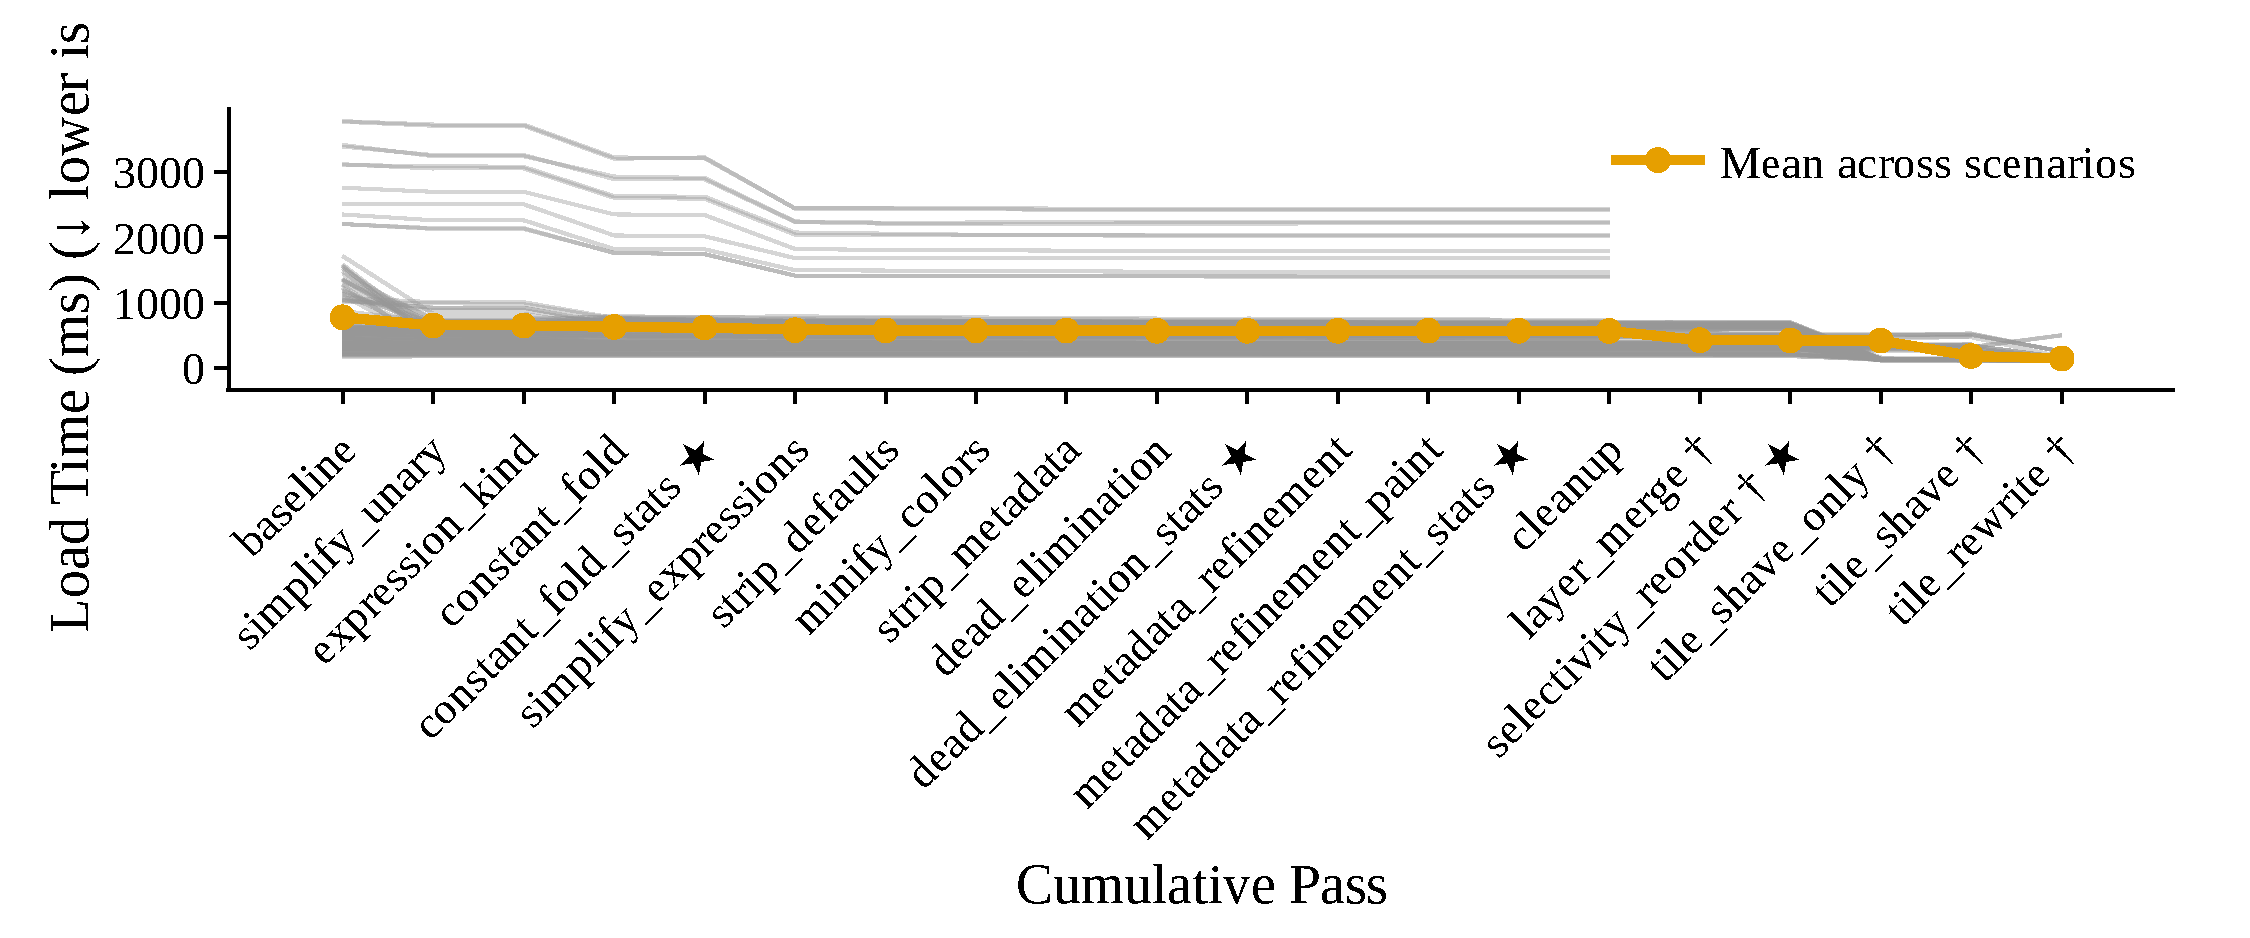
\includegraphics[width=\linewidth]{figures/waterfall_loadMs.pdf}
    \caption{
Cumulative ablation waterfall for load time.
Each bar shows the median change introduced by adding one expression pass on top of all previous passes, aggregated across all 18 scenarios and 15 benchmark styles.
We can see that in the extremes, unary simplifcation has the largest effect.
The aggregate load-time improvement across all expression passes is modest (\qty{-1.8}{\percent}), with expression passes serving primarily as enablers for downstream structural and data-level passes.
For caveats, please see \cref{sub:expr_discussion}}
    \label{fig:waterfall_loadMs}
\end{figure}

\begin{figure}[htbp]
    \centering
    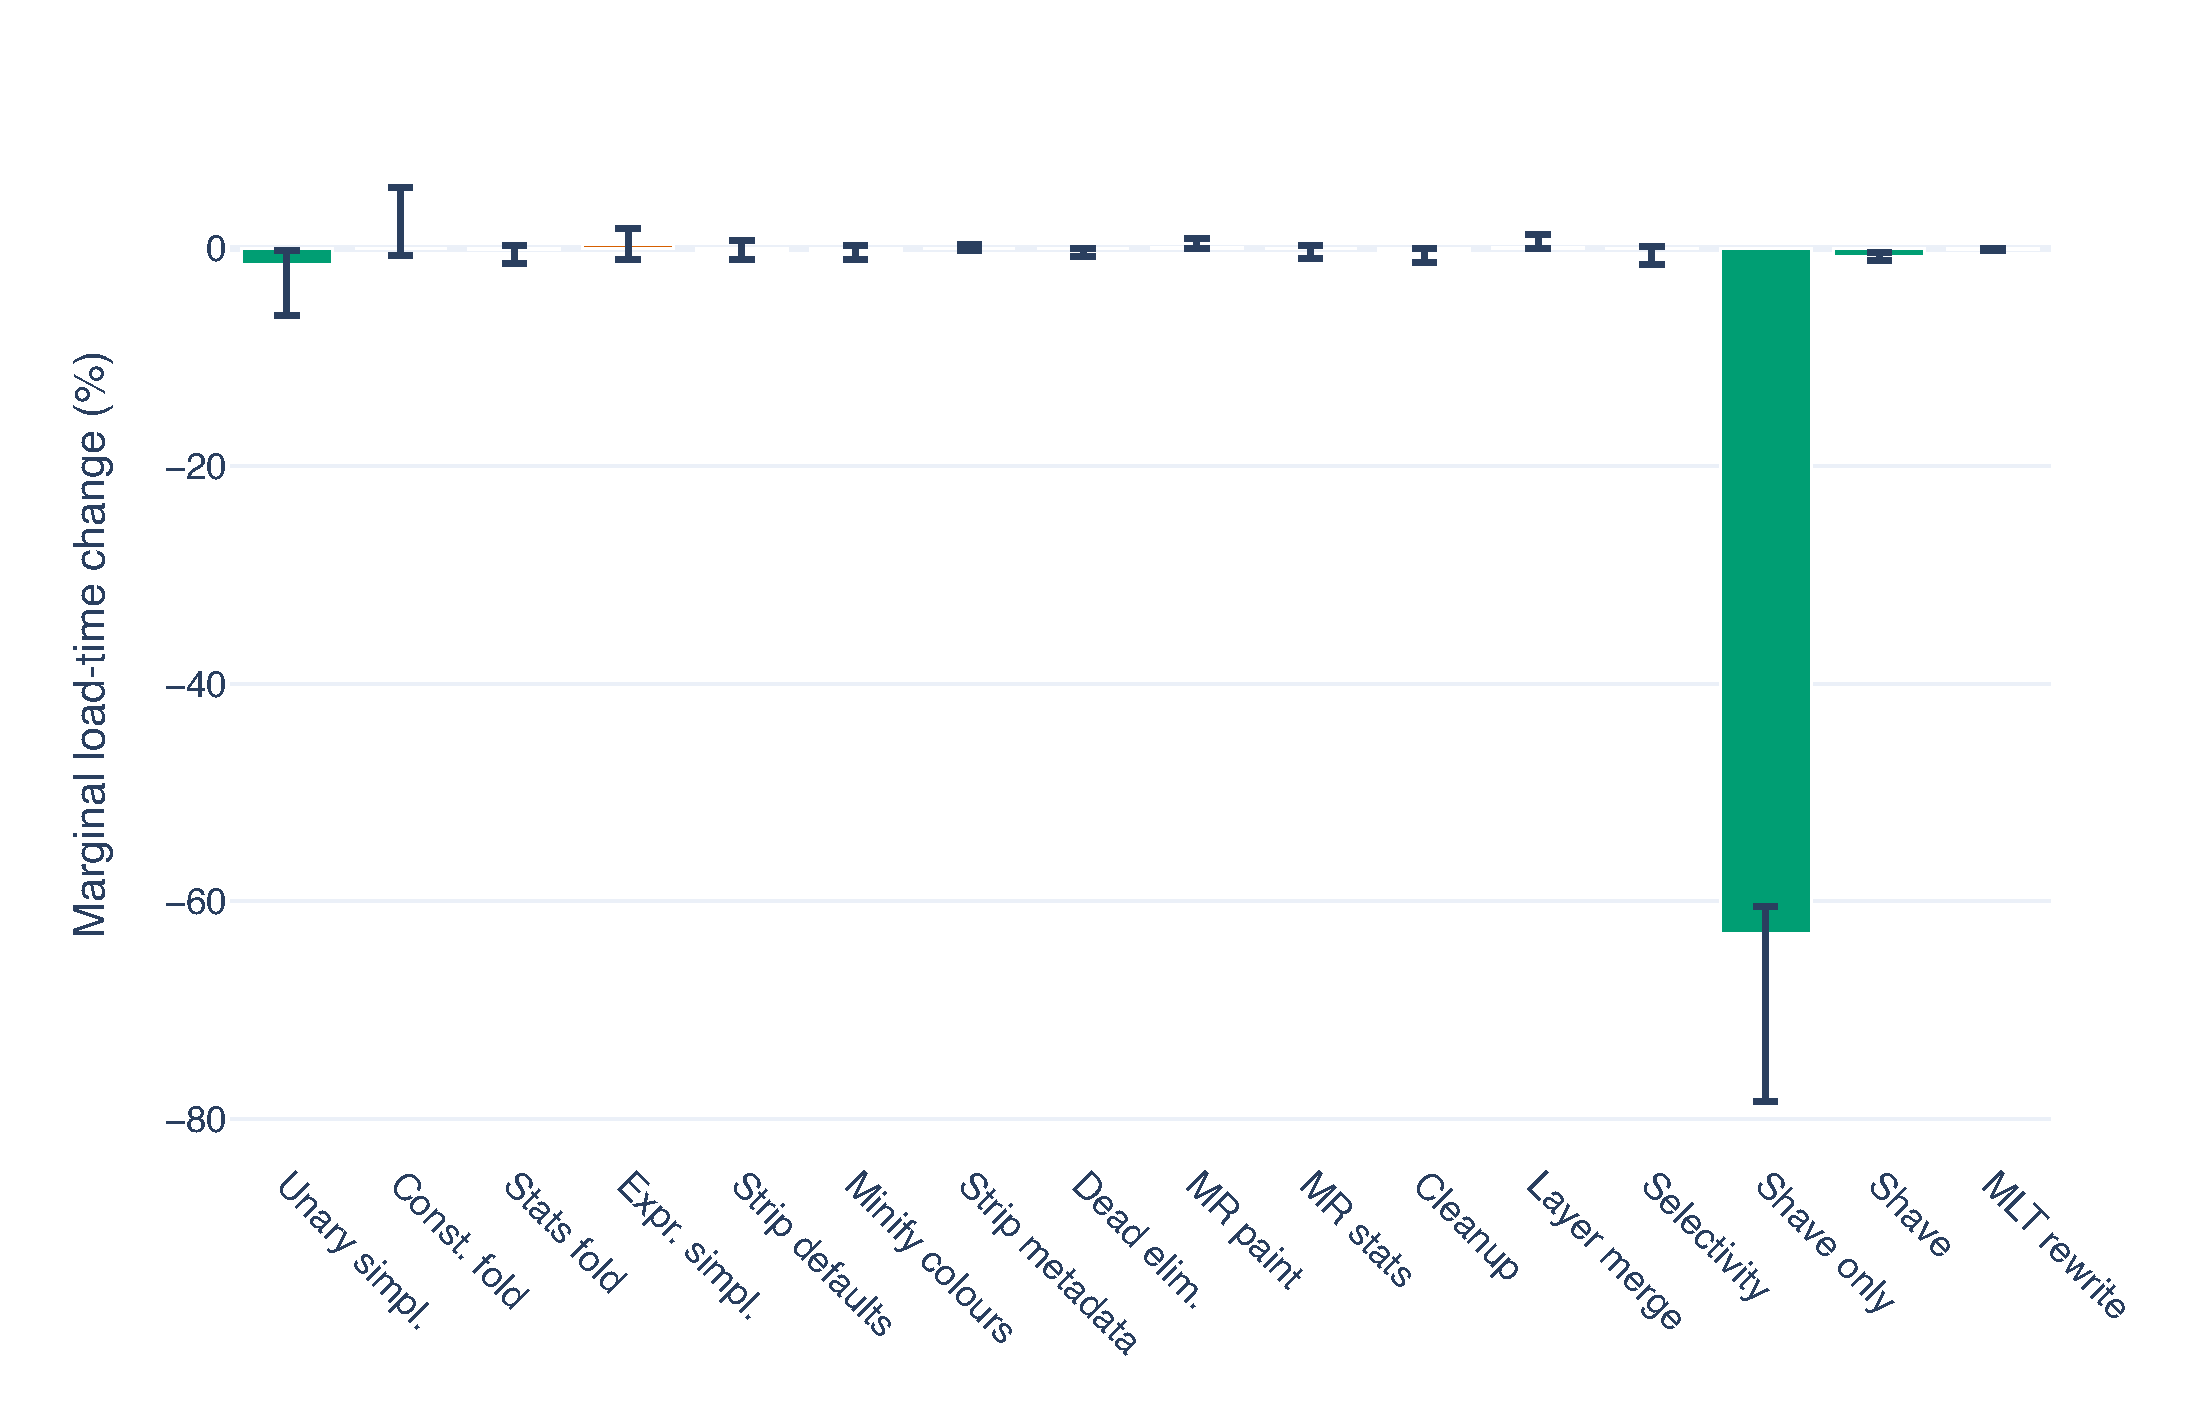
\includegraphics[width=\linewidth]{figures/marginal_loadMs.pdf}
    \caption{
Marginal contribution of each expression pass to load time reduction shows the effect of each of the passes cleanly. }
    \label{fig:marginal_loadMs}
\end{figure}

\begin{figure}[htbp]
    \centering
    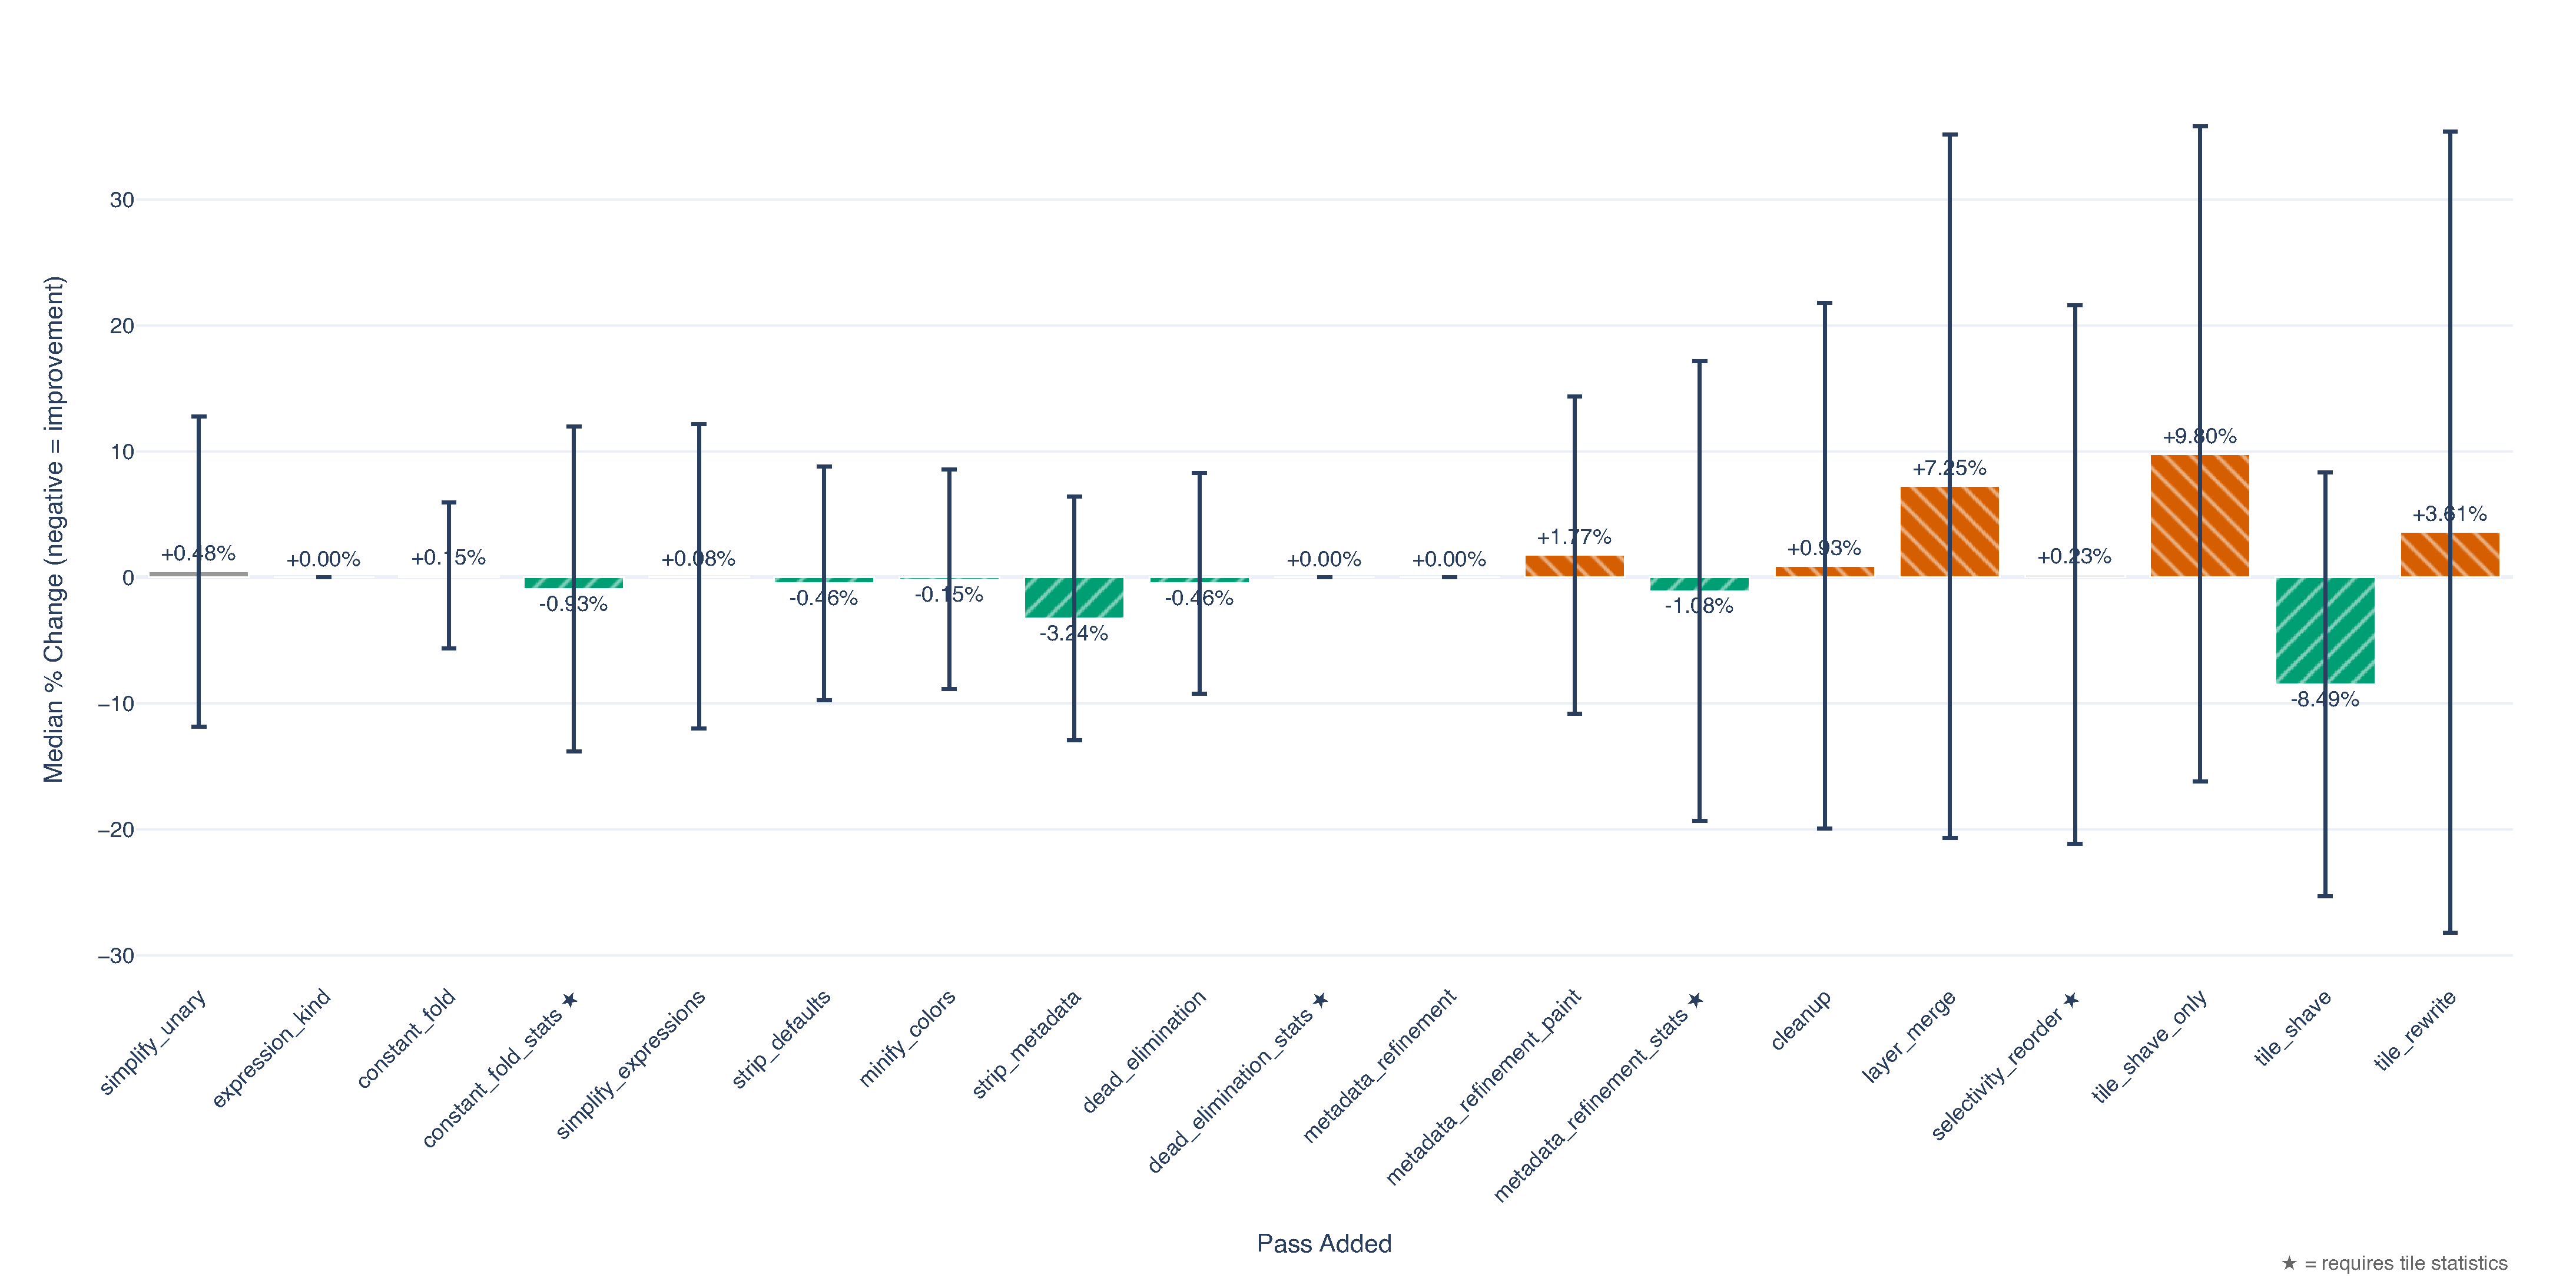
\includegraphics[width=\linewidth]{figures/marginal_styleParseMs.pdf}
    \caption{
Marginal contribution of each expression pass to \texttt{styleParseMs}.
The size-reducing passes (default stripping in particular) shorten the parse step monotonically, even where their end-to-end load-time effect is within noise.
This is the proximate mechanism behind the style-parse leg of the time breakdown in \cref{fig:time_breakdown}.}
    \label{fig:marginal_styleParseMs}
\end{figure}

\subsection{Discussion}\label{sub:expr_discussion}

Expression passes shave only \qty{1.8}{\percent} from median load time, but raw style size drops by up to \qty{20.3}{\percent} on Fiord, with most of the size win concentrated in a single pass (default stripping).
We use the rest of this section to explain why one outlier pass dominates the per-style picture and why the size-reduction story diverges from the rendering-time one.

\paragraph{Dominance of Unary Simplification}
Some styles are implemented in a not optimal way and thus allow a very high unary simplification gain.
The gain of this simplification is non-representative and biases the results to look better than they are overall.
Only two of the style familys gain significant speedups, both of the times through what we think are typos in how the style is written.

We expect this.
Reducing an expression tree to a literal eliminates all per-feature evaluation cost for that expression, whereas algebraic simplifications merely shorten the evaluation path.
For some styles this does not hold and unary simplification is more effective due to expensive string index handling being collapsed into senatically identical, but faster variants.
Fixpoint iteration amplifies the effect.
A single successful simplfication can cascade through nested expressions, collapsing entire subtrees in subsequent iterations.

\paragraph{Size Reduction vs.\ Rendering Improvement}
Passes that primarily reduce serialized style size (default stripping, color minification) show smaller rendering improvements but contribute meaningfully to transfer size under compression.
This primarily benefits time to first render (discussed in \cref{sub:combined_marginal}).
We note the distinction between raw, gzip, and Brotli reductions: some rewrites (e.g., \mlop{\texttt{any}}$\to$\mlop{\texttt{in}}) increase raw token count while decreasing compressed size, because the repetitive structure of \mlop{\texttt{in}} operand lists compresses well.

\paragraph{Empirical Coverage of Selectivity Reordering}
Selectivity reordering (step~16) is a theoretically motivated heuristic whose isolated rendering impact we did not measure in this evaluation.
Because it appears late in the cumulative ablation, its marginal contribution is confounded with the preceding passes.
We acknowledge the independence assumption underlying the selectivity estimates as inaccurate for correlated map predicates (\cref{sec:query_optimizations}), and the empirical benefit may be negligible for styles whose filters are already short.

\paragraph{Downstream Interaction with the Data Pipeline}
Beyond their direct rendering benefit, expression-level simplifications feed into the data-level pipeline evaluated in \cref{sec:exp_mlt}.
Each folded filter predicate and each pruned \mlop{\texttt{match}} arm reduces the set of property names and categorical values that the tile pruning advisory (\cref{sub:tile_shaving}) must track.
Each filter reduced to \mlval{\texttt{false}} enables dead layer elimination in the structural phase, which removes that layer's entire property footprint from the advisory.
Simpler filters are also more amenable to the advisory's static analysis, because canonical forms (e.g., a direct \texttt{[\mlop{"=="},~\ldots]} rather than a double-negated comparison) expose referenced property values more readily.
The magnitude of this interaction is quantified in \cref{sec:exp_mlt}.


\section{Experiment 2: Structural Optimizations}\label{sec:exp_structural}
\begin{keytakeaways}
\item Dead-layer elimination and layer merging produce nearly all the structural-family gains;\newline
      the other passes are negligible on their own.
\item Layer merging can grow raw bytes yet still shrink frame time.
Gzip absorbs the difference.
\item Symbol-heavy styles benefit less because symbol layers are excluded from merging.
\end{keytakeaways}

\noindent Where the previous experiment rewrote local expressions, in this one we evaluate the passes that reason across layers and sources: the structural family of \cref{sub:structural_optimizations}.

\subsection{Pass Interactions}\label{sub:structural_interactions}

Several pairwise dependencies between structural passes shape what we measure in the cumulative ablation in \cref{sub:structural_results}.
Expression passes must run first so that metadata refinement sees zoom predicates in their canonical form.
Dead elimination must precede layer merging because a dead layer between two otherwise-mergeable live layers blocks the merge.
Similarly, metadata refinement must precede cleanup so the residual \mlval{\texttt{true}} filters and zero-opacity layers it produces can be removed.
We give the full ordering rationale in \cref{sub:pipeline}.
The practical consequence here is that the marginal contribution of each later pass in the ablation will reflect work that an earlier pass enabled, not just the pass itself.

\subsection{Evaluation}\label{sub:structural_evaluation}

Structural passes correspond to ablation steps~8-15 within the cumulative ablation of \cref{sub:ablation}.
In addition to the rendering metrics from Experiment~1 (\cref{sub:metrics}), we report complexity metrics for the structural evaluation: layer count, filter count, and total expression node count.
We report the effects on performance generalized in \cref{sub:cross_results} (over the generalization corpus of \cref{sub:generalization_corpus}) and the effect of the expression-level steps this work builds upon in \cref{sec:exp_expressions}.

\subsection{Results}\label{sub:structural_results}

\cref{fig:complexity_layer_count} tracks layer count across the structural ablation steps, showing which passes concretely remove layers rather than merely rewriting them.
\cref{fig:complexity_total_expression_nodes,fig:complexity_filter_count} extend the complexity view to the two remaining metrics introduced in \cref{sub:structural_evaluation}: total expression-tree node count and filter count.
\cref{fig:style_size_ablation} complements these with the raw, gzip, and Brotli style sizes, confirming that the structural reductions also translate into smaller transfer size rather than just reshuffling the serialized form.


\begin{figure}[htbp]
	\centering
	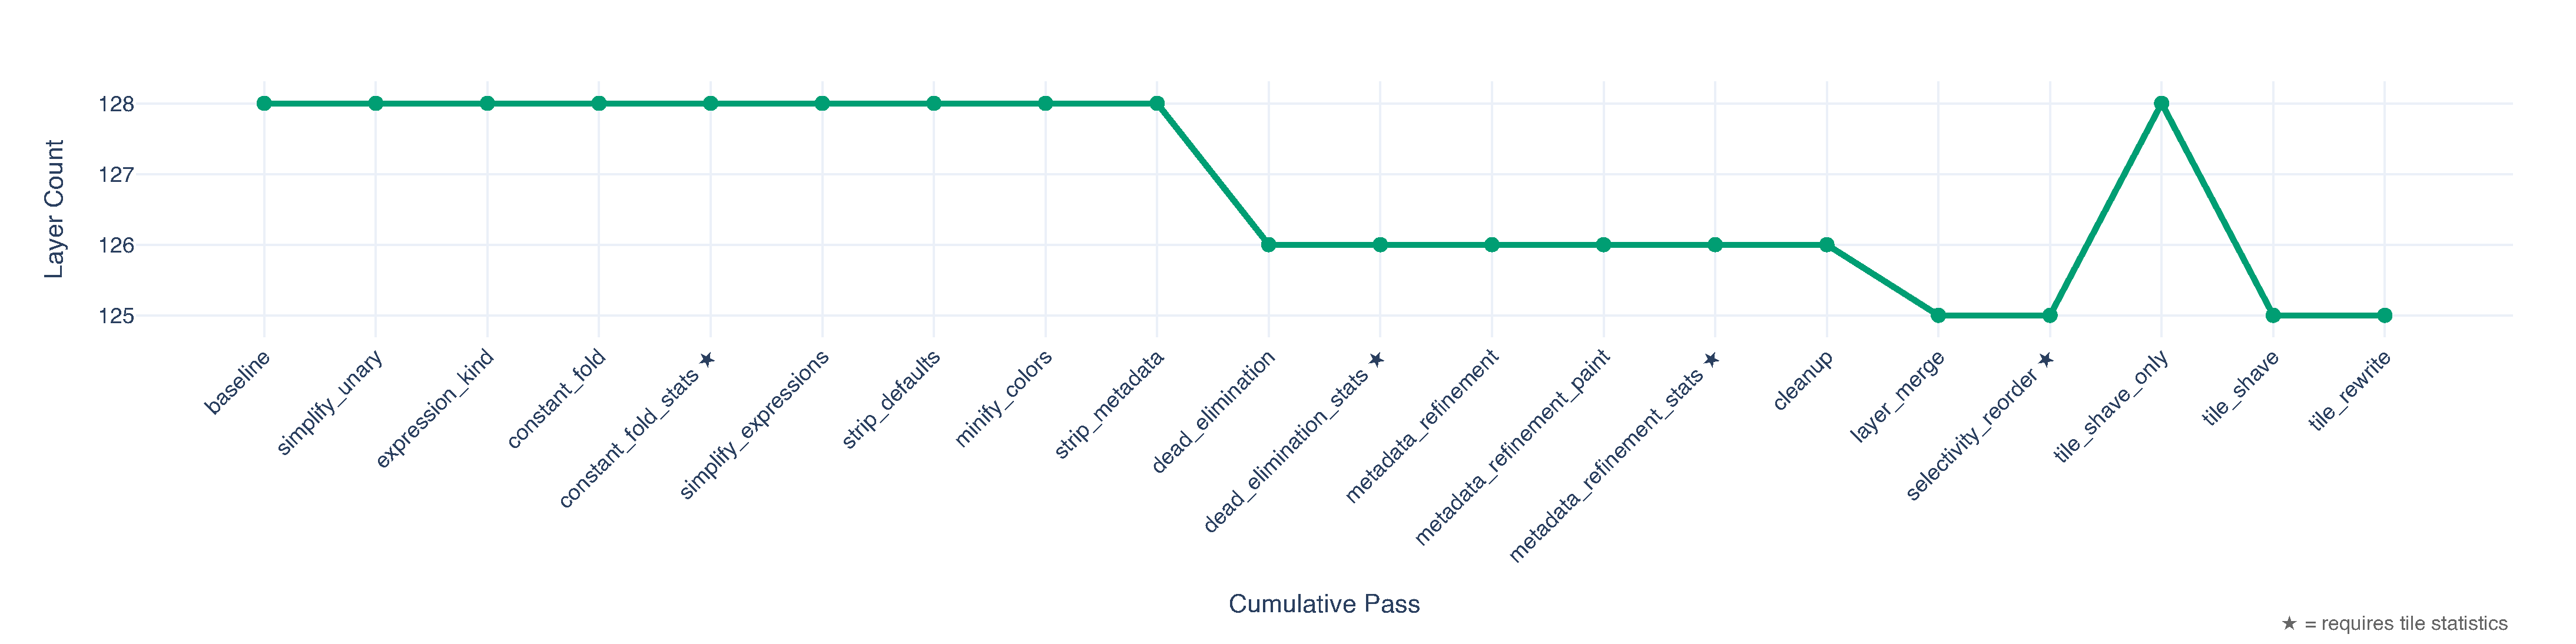
\includegraphics[width=\linewidth]{figures/complexity_layer_count.pdf}
	\caption{
Layer Count across Cumulative Ablation Steps on the Liberty Style: only layer merging reduces the layer count.
Dead elimination rarely removes whole layers, because styles are designed to expose parts of the map rather than leave entire layers unreferenced.}
	\label{fig:complexity_layer_count}
\end{figure}

\begin{figure}[htbp]
	\centering
	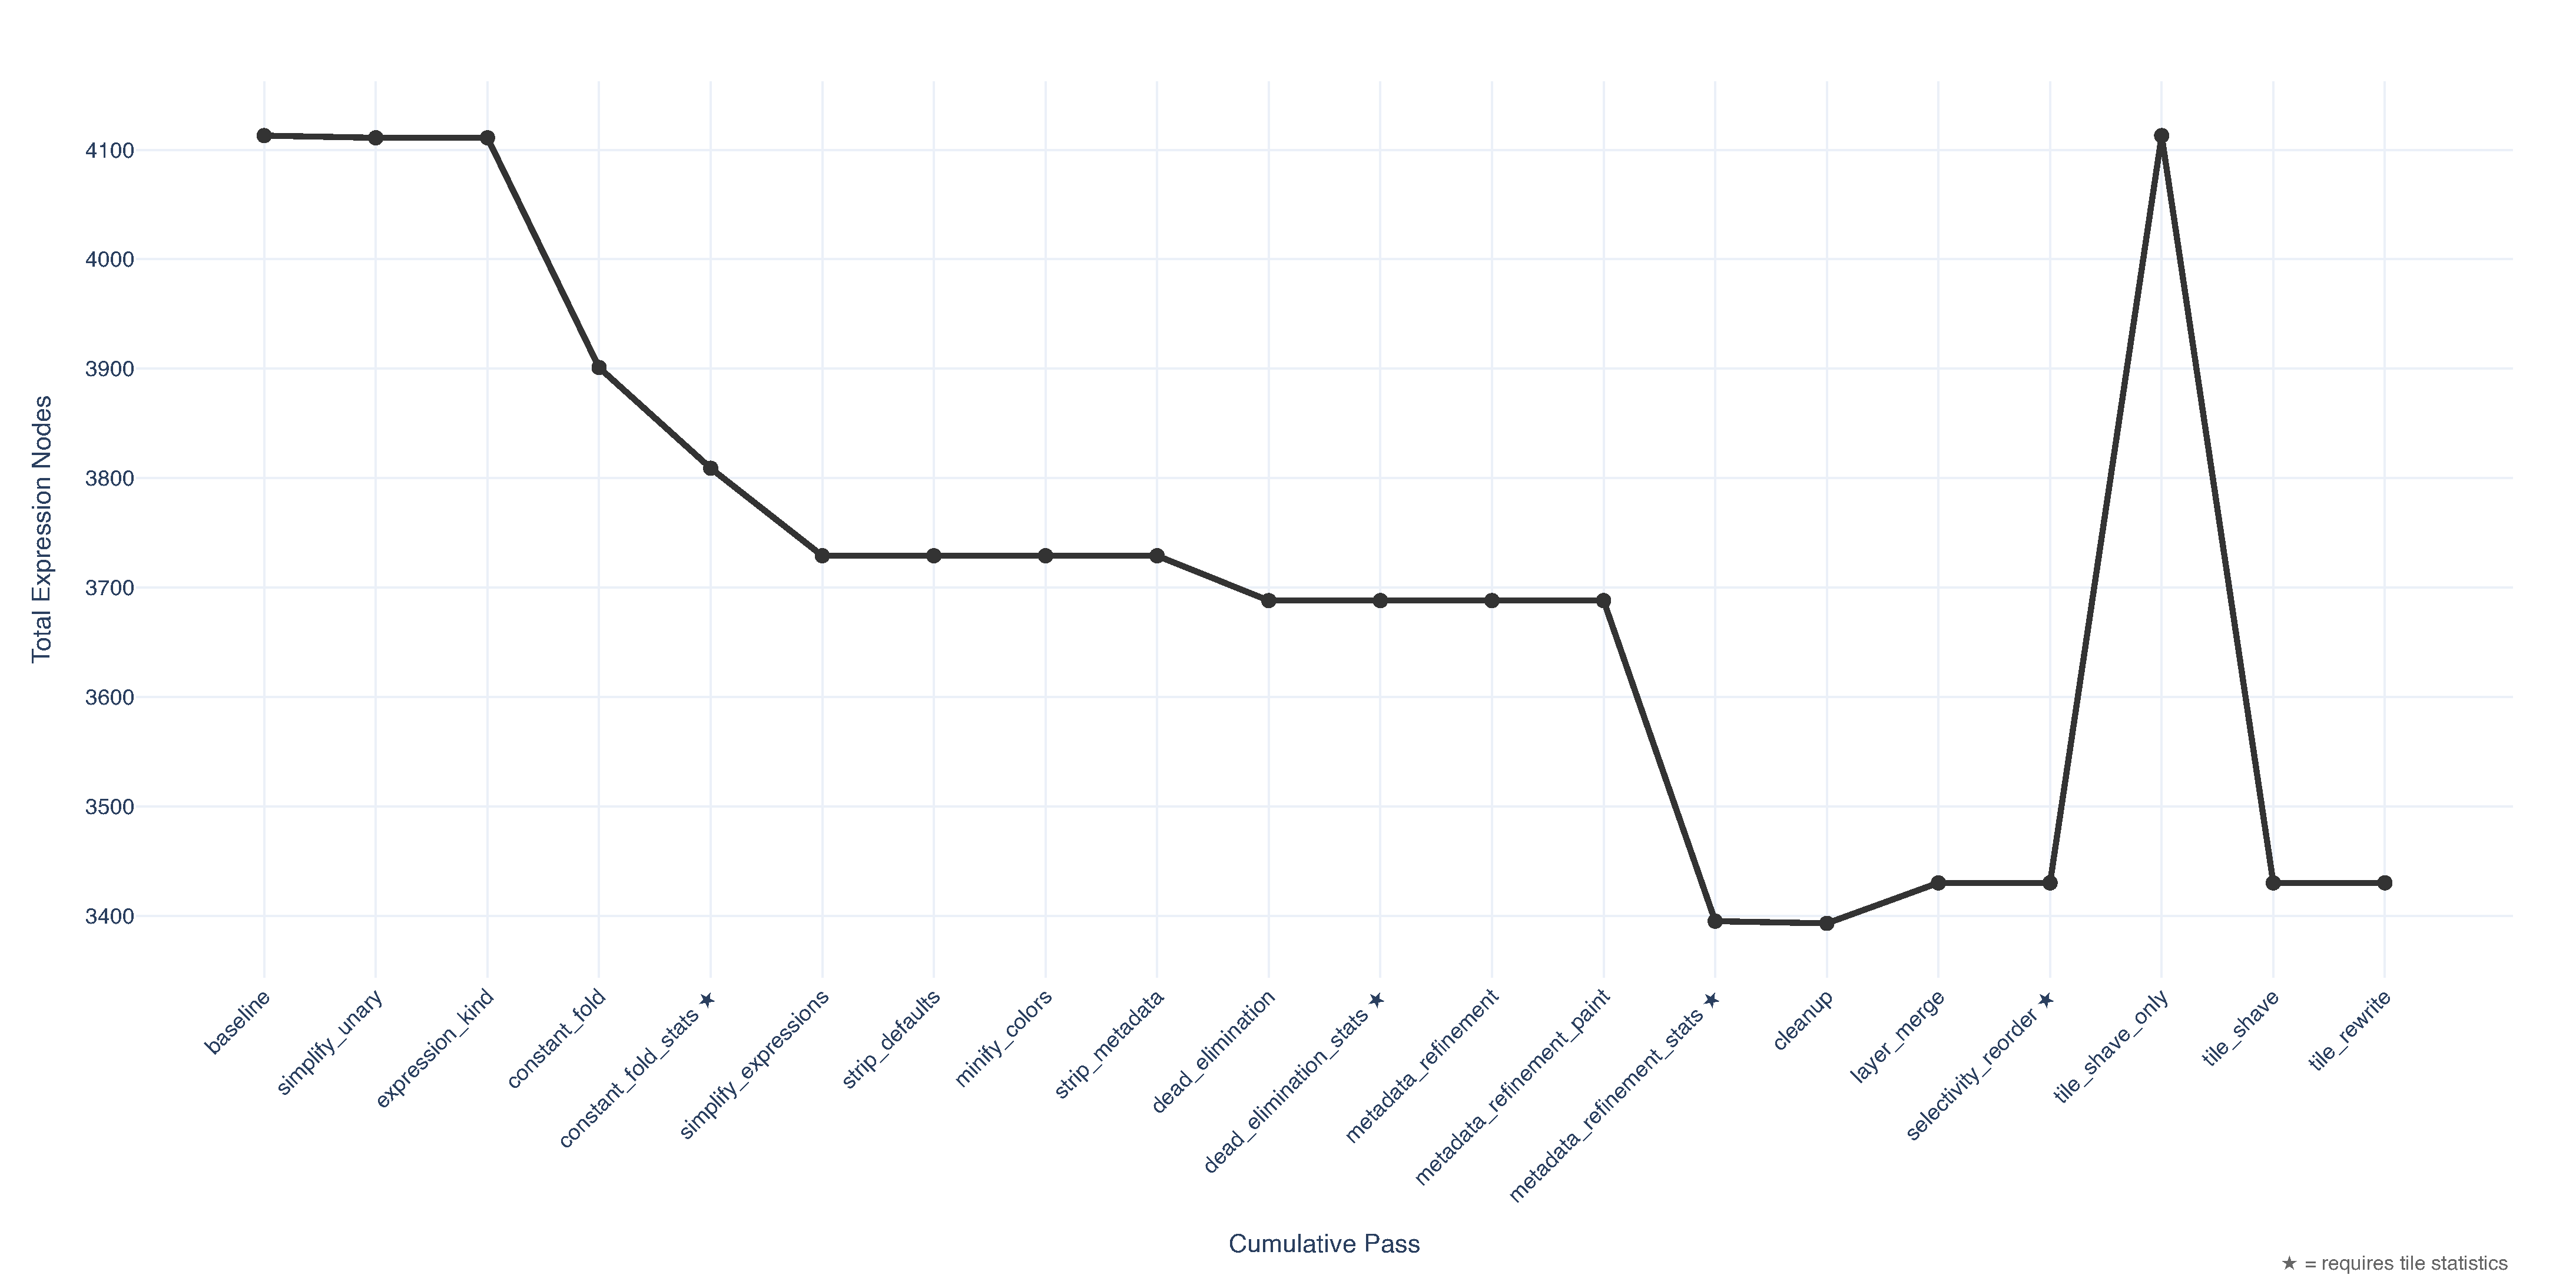
\includegraphics[width=\linewidth]{figures/complexity_total_expression_nodes.pdf}
	\caption{
Total expression-tree node count across cumulative ablation steps.
Expression passes (steps~1-7) produce the largest reductions, with Fiord dropping by \qty{36.8}{\percent} (\num{1610}$\to$\num{1018}) and Liberty by \qty{10.5}{\percent} (\num{3537}$\to$\num{3167}).
Structural passes contribute additional, smaller reductions by removing or merging layers that own subtrees.}
	\label{fig:complexity_total_expression_nodes}
\end{figure}

\begin{figure}[htbp]
	\centering
	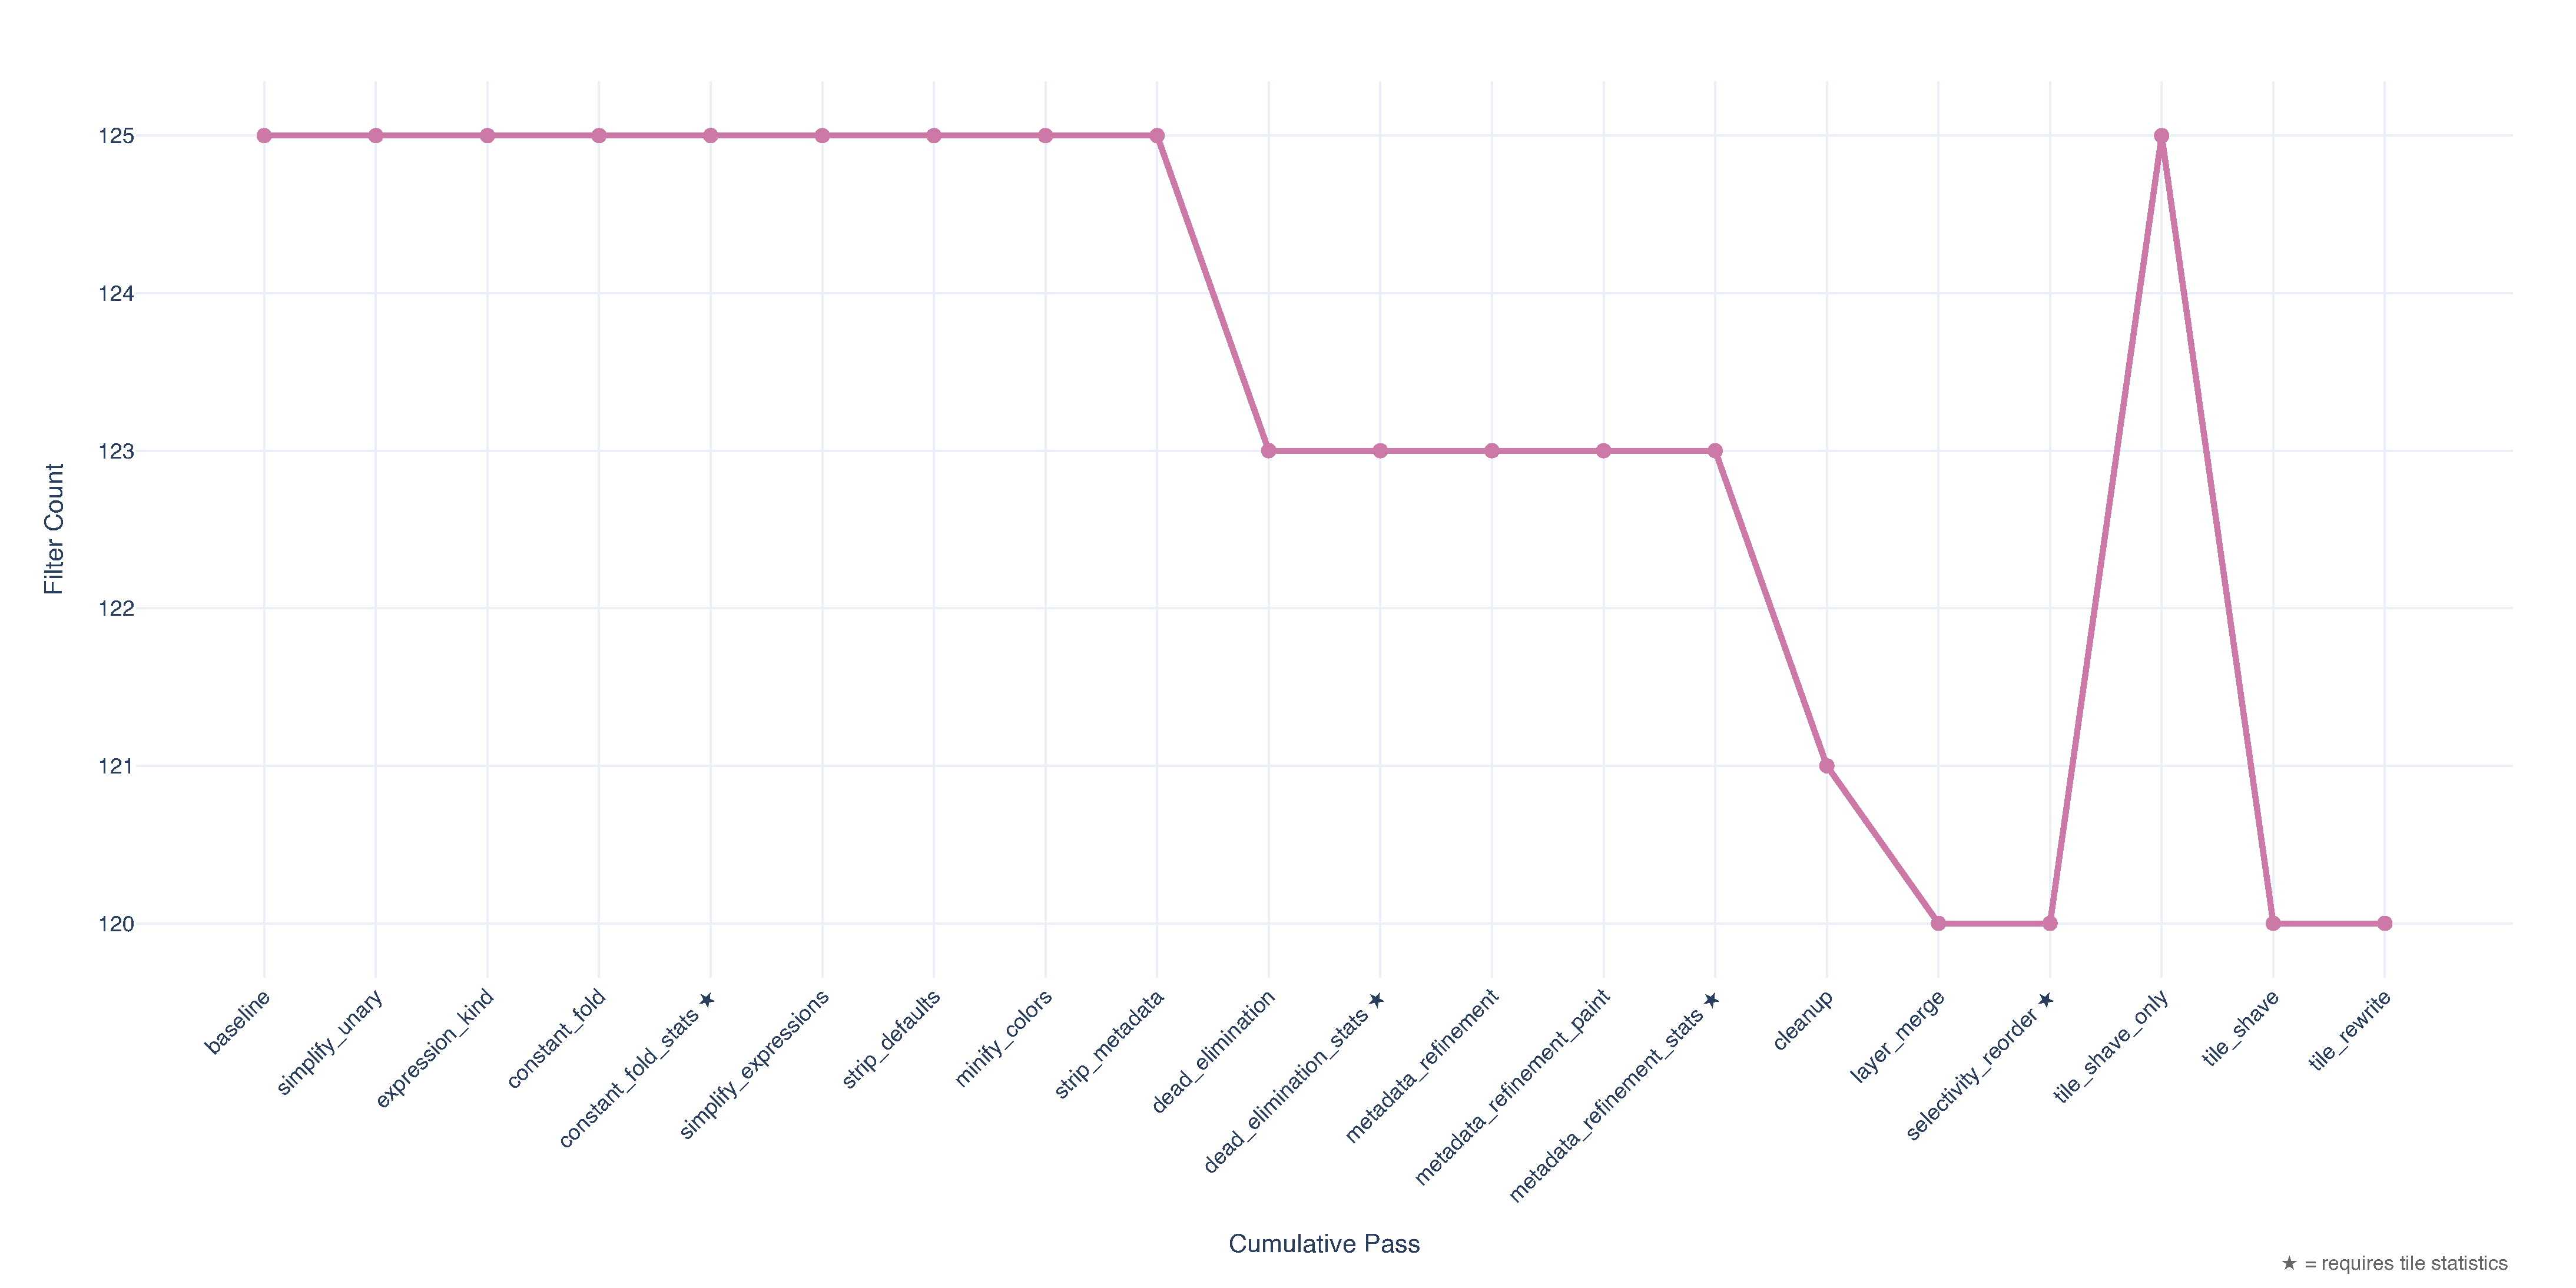
\includegraphics[width=\linewidth]{figures/complexity_filter_count.pdf}
	\caption{
Filter count across cumulative ablation steps.
Metadata refinement (consuming zoom predicates) and dead elimination drive most of the filter-count reduction.
Cleanup removes the residual \mlval{\texttt{true}} filters that refinement leaves behind.}
	\label{fig:complexity_filter_count}
\end{figure}

\begin{figure}[htbp]
	\centering
	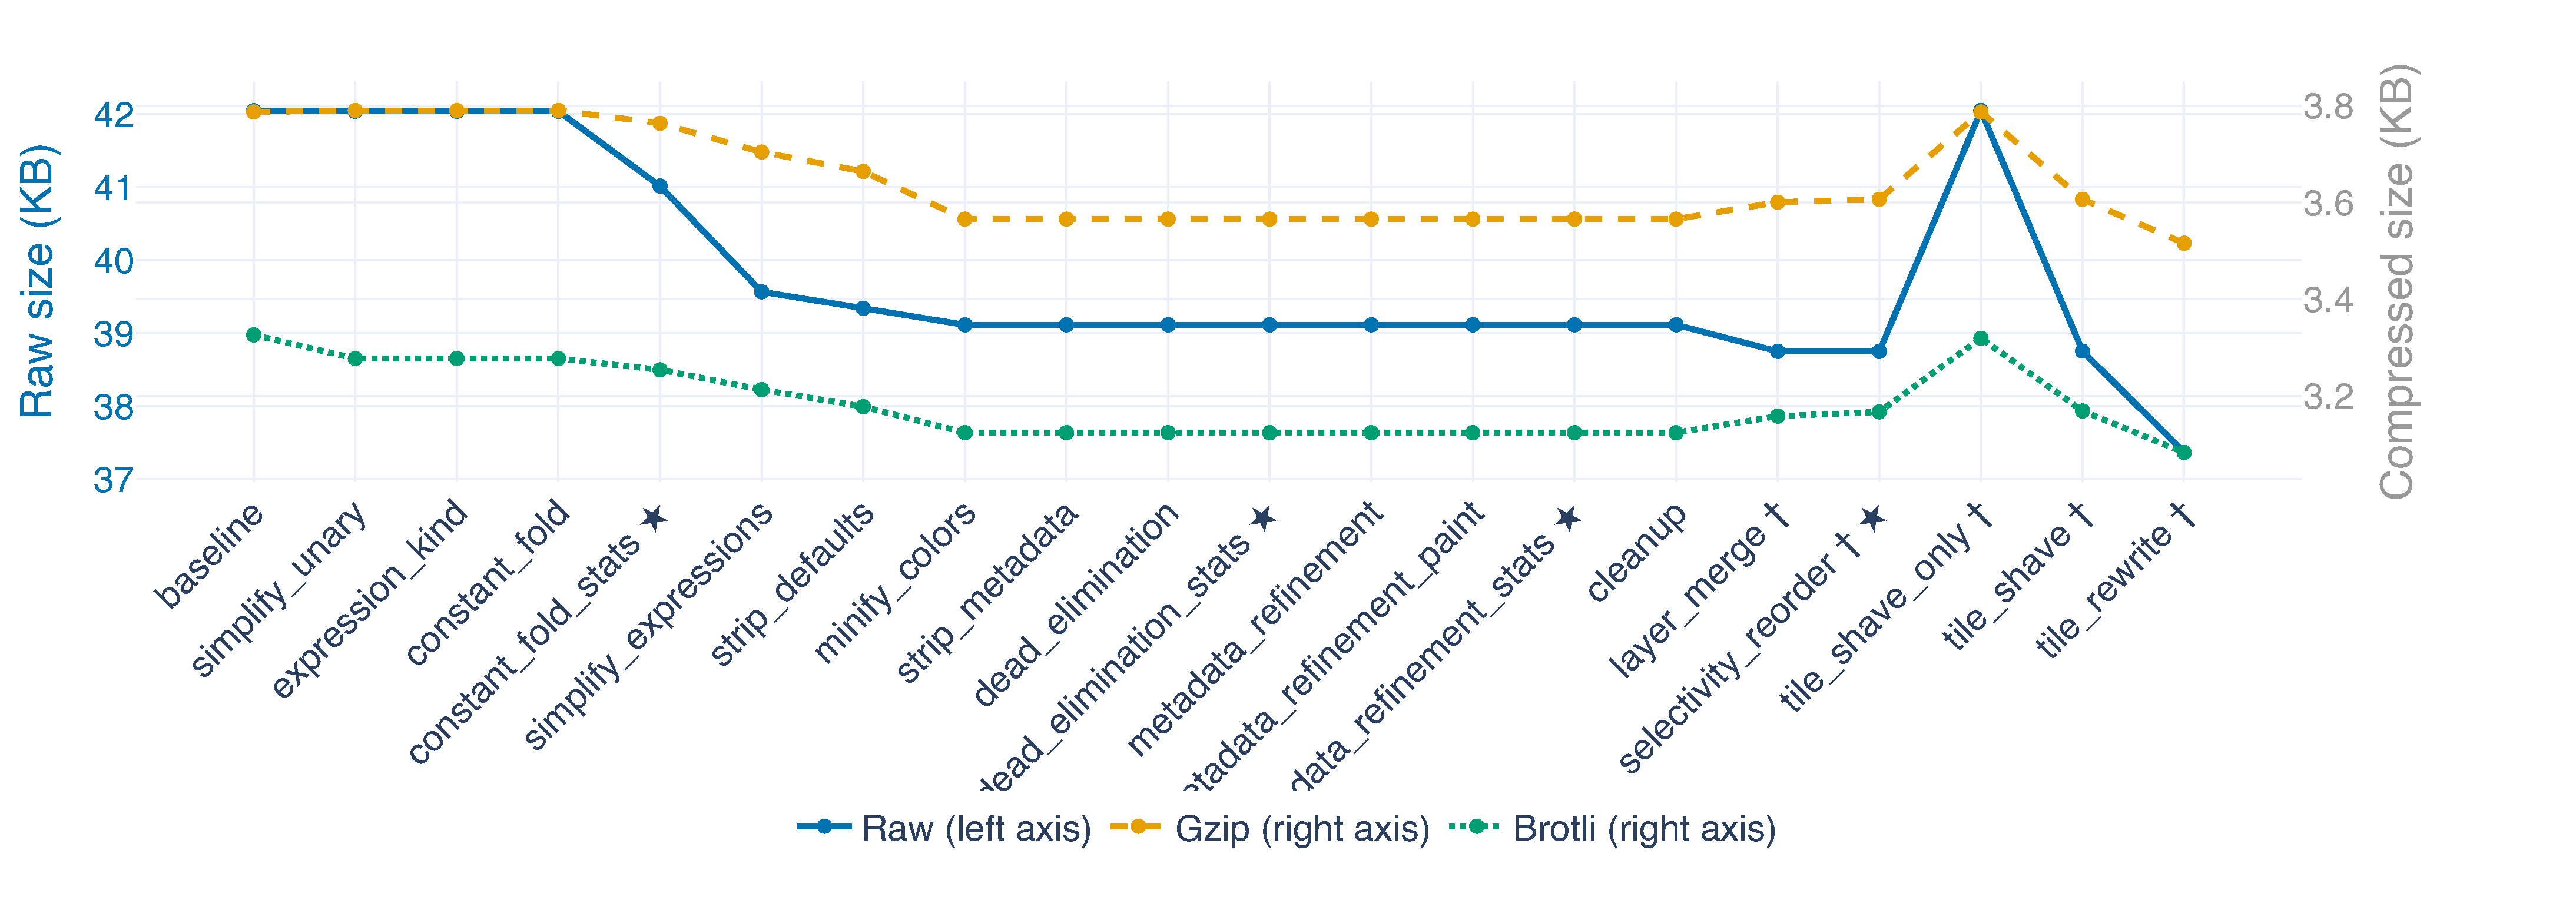
\includegraphics[width=\linewidth]{figures/style_size_ablation.pdf}
	\caption{
Style size (raw, gzip, Brotli) across ablation steps: the effect on this metric is incremental rather than transformative.}
	\label{fig:style_size_ablation}
\end{figure}

The magnitude of structural improvement is style-dependent.
Fiord's 48-layer style sheds two layers (\qty{-4.2}{\percent}), one from dead elimination (step~9) and one from cleanup (step~14) after metadata refinement reduces a filter on an invisible layer to \mlval{\texttt{true}}.
The drop translates to \qty{-14.1}{\percent} gzip transfer and \qty{-36.8}{\percent} fewer expression-tree nodes (\num{1610}$\to$\num{1018}).
Liberty's 111 layers shed four (\qty{-3.6}{\percent}), concentrated in the layer-merge step (step~15), which combines four pairs of adjacent layers with compatible filters for \qty{-4.9}{\percent} gzip and \qty{-10.5}{\percent} nodes (\num{3537}$\to$\num{3167}).
Layer merging itself adds \qty{36}{\byte} of gzip because the merged filter expressions are wordier.

\subsection{Discussion}\label{sub:structural_discussion}

Two of the six structural passes (dead-layer elimination and layer merging) produce nearly all of the gain, cutting Fiord's gzip transfer by \qty{14.1}{\percent} and Liberty's by \qty{4.9}{\percent}.
The following paragraphs unpack why those two dominate and how the remaining passes contribute indirectly or feed into the data-level pipeline downstream.

\paragraph{Dominance of Dead Elimination and Layer Merging}
Among the structural passes, dead elimination and layer merging produce the largest improvements in both rendering performance and style complexity.
Dead elimination directly reduces the number of layers the renderer must process per frame.
Layer merging reduces draw calls by combining multiple rendering passes into one.
The interaction between the two is synergistic: styles with many narrowly-filtered layers (e.g., road styles that define separate layers for each road class) benefit most, as dead elimination first removes layers for road classes absent from the data, and layer merging then combines the remaining layers into a single multi-class layer.

\paragraph{Size vs.\ Runtime Trade-Off in Layer Merging}
Layer merging does not always reduce the raw serialized byte count.
A merged layer replaces $k$ small filter expressions with a single \mlop{\texttt{match}}-keyed filter and $k$-armed \mlop{\texttt{match}} expressions for every differing paint property, which for small $k$ can produce a slightly larger textual representation than the sum of the originals.
The per-style ablation tables in \cref{sec:app_per_style} show one such case (Bright: \num{44.4}$\to$\qty{44.6}{\kilo\byte} after layer merging), where the raw count creeps up while the layer count drops by one (119$\to$118).
This was uncomfortable when we first saw it in the runs, since the intuition is that merging should shrink the style, but raw byte count turns out to be a proxy for parse time and transfer cost rather than for rendering cost, which is driven by layer count and per-frame draw calls.
The merged layer is still cheaper to render even when its serialized form is bigger, and the gzip and Brotli columns of the same table show the compressed size essentially unchanged, so the raw increase disappears under realistic wire compression anyway.

\paragraph{Indirect Effects of Metadata Refinement}
Metadata refinement does not directly reduce the number of layers or the complexity of expressions.
Instead, it enables the renderer to skip layers at zoom levels where they are invisible.
The rendering improvement is therefore zoom-dependent.
At overview zoom levels (where many layers are filtered out by tightened \texttt{minzoom}) the improvement is large, and at street-level zoom (where most layers are active) the improvement is smaller.
Paint-based refinement captures a class of optimizations that are invisible to filter analysis.
A layer whose opacity interpolates from~0 at zoom~12 is indistinguishable from a fully visible layer when examining only the filter.

\paragraph{Amplification of Style-Only Passes by Stats-Driven Passes}
The marginal contribution of stats-driven dead elimination (step~10) over non-stats dead elimination (step~9) quantifies the value of tile statistics for style optimizations.
Styles that use broad \texttt{source-layer} references benefit most, as statistics reveal which geometry types and property values actually exist.
For styles that already have precise filters (e.g., hand-tuned Americana), the marginal gain is smaller.

\paragraph{Symbol Layer Exclusion}
We exclude symbol layers from merging because MapLibre's collision detection operates per-layer (we give the soundness argument in \cref{sub:structural_optimizations}).
The headline merging numbers above are therefore reductions in the non-symbol pool only.
Because styles are usually dominated by labels, most see proportionally smaller layer-count gains.

\paragraph{Downstream Interaction with Tile Shaving}
Dead layer elimination has a second-order effect beyond reducing per-frame draw calls:
each eliminated layer removes its property references from the tile pruning advisory computed in the data-level pipeline (\cref{sub:tile_shaving}).
If a removed layer was the sole consumer of a property column, that column is stripped from every tile at encoding time.
Similarly, metadata refinement's tightened zoom bounds cause the advisory to mark additional zoom levels as unused for a given source-layer, potentially eliminating entire tiles.
We characterize this interaction fully in \cref{sub:mlt_discussion} and quantify it in \cref{sub:mlt_results}.
The aggregate data shows that the composition is additive rather than synergistic, but the advisory-narrowing effect is a necessary precondition for style-dependent tile shaving.


\section{Experiment 3: Data-Level Optimizations}\label{sec:exp_mlt}
\begin{keytakeaways}
\item Tile shaving dominates with a \qty{-71.5}{\percent} median load reduction, and style passes contribute additively, not synergistically.
\item The \ac{MLT} format alone is not the win.
The reference \ac{MLT} encoder drifts above $1.0\times$ \ac{MVT} under gzip/Brotli.\newline
    The gain comes from the strategy competition and shared-dictionary selection in our encoder.
\end{keytakeaways}

\noindent In \cref{sec:exp_structural,sec:exp_expressions} we optimized the \emph{program} the renderer executes.
In this experiment we ask whether we can optimize the \emph{data} it consumes using the same style information, and to what extent the two levels interact.
This is the joint-optimization question at the heart of Research Goal~R1 and formalised in \cref{sec:problem_statement}.
The data-level pipeline we apply here (\cref{sub:data_optimizations}) takes the optimized style and uses it to drive the tile pruning advisory and the encoding strategy competition.

\textit{We carried out this experiment in collaboration with Rivian Automotive, Inc to optimize performance, correctness, and software architecture of the encoder-decoder pair.
We implemented the encoder and its strategy-selection routine ourselves.
Rivian contributed the runtime performance engineering, which brings transcoding of the Germany OpenMapTiles tileset down from roughly five hours under the prior Tremmel \& Zink reference encoder to about one minute.
We credit that speedup to Rivian rather than ourselves, and therefore do not analyse encoder performance further in this chapter.}

\subsection{Problem Statement}\label{sub:mlt_problem}

Beyond the thesis-wide formal optimization problem of \cref{sec:problem_statement}, two open problems specific to the data-level pipeline frame this experiment:

\begin{enumerate}
    \item \textbf{Tiles carry data the style never uses, and how much depends on the style.}
    A general-purpose tile schema (e.g., OpenMapTiles) exposes hundreds of properties and multiple geometry types.
Any specific style references only a fraction.
    The unused remainder is style-dependent, so the savings achievable by tile shaving (\cref{sub:tile_shaving}) co-vary with the upstream style optimizations:
    more dead layers and simpler filters expose more removable columns and feature values.

    \item \textbf{Encoders ignore the data characteristics that shaving produces.}
    Existing \ac{MLT} encoders commit to a fixed encoding plan per column.
    After shaving, the surviving data has fewer distinct values, longer runs, and smaller string vocabularies, which a data-adaptive encoder (\cref{sub:encoding_strategies}) can exploit but a fixed-plan encoder cannot.
\end{enumerate}

\subsection{Evaluation Design}\label{sub:mlt_evaluation}

In this experiment we isolate the interaction between style-level and data-level optimizations and identify which level contributes the dominant share of the end-to-end savings.
We use a cumulative design with five configurations, each adding one optimization layer:

\begin{enumerate}
    \item \textbf{\ac{MVT} baseline}: unoptimized protobuf-encoded tiles served with the original style.
    \item \textbf{Style-only}: the optimized style from Experiments~1-2, served with unmodified \ac{MVT} tiles.
    \item \textbf{Shaving-only}: the original style with tile shaving applied (advisory-driven pruning of unused columns, geometry types, and property values), but without style optimizations.
    \item \textbf{Style + shaving}: The optimized style driving tile shaving.
    Dead layer elimination and metadata refinement may narrow the advisory relative to the unoptimized style.
    \item \textbf{Style + shaving + \ac{MLT} encoding}: encoding stage that delivers the shaved data to the wire via automatic encoding strategy selection (sort competition, per-stream profiling, string compression).
\end{enumerate}

\noindent Configurations~2-4 isolate the interaction effect.
If the combined reduction of style+shaving exceeds the sum of style-only and shaving-only, the two optimization categories are synergistic.
If approximately equal, they compose additively.
If less, they are partially redundant.
Configuration~5 adds the encoding layer: after shaving has determined what data survives, the multi-strategy competition adapts to the statistical properties of the surviving data.
Those properties differ from the unshaved original because shaving has removed columns and features, altering value distributions and run-length characteristics.

For each configuration, we collect two classes of metrics: \emph{tile transfer metrics} (encoded tile size in raw, gzip, Brotli per zoom level, total tileset volume, and encoding time per tile) and \emph{rendering metrics} shared with Experiments~1-2 (load time, frames per second, frame time percentiles p50/p95/p99, and time to first tile), enabling direct comparison of data-level contributions against expression-level and structural contributions in the combined analysis (\cref{sec:exp_combined}).

\subsection{Results: Style-Driven Cascade}\label{sub:mlt_results}

In this section we quantify the interaction between style-level and data-level optimizations previewed in \cref{sub:structural_discussion}: style-level optimizations narrow the pruning advisory, and in the following paragraphs we measure the extent of this effect before turning to the encoding evaluation.

\paragraph{Interaction between Style and Data Optimizations}
Comparing gzip-size reductions for style-only, shaving-only, and the combination: Fiord's combined reduction (\qty{14.7}{\percent}) sits \qty{0.2}{\percent} above its style-only figure (\qty{14.5}{\percent}), and Liberty's combined (\qty{4.8}{\percent}) matches its style-only (\qty{4.8}{\percent}).
Both styles compose additively.
Shaving alone is negligible for these two because Liberty references most tile properties and Fiord's gains already come from layer-level cleanup.
This was the central empirical question of the thesis and the one we expected to answer in the affirmative going in.
The data returned additivity, not synergy.
Per-scenario load-time synergy (combined exceeding the sum) appears in 17 of 36 style-scenario pairs but is too sparse to lift the aggregate.

\paragraph{Rendering Metrics across Configurations}
\cref{fig:rendering_metrics_mlt} reveals that the dominant rendering improvement comes from tile shaving rather than style optimizations.
Headline numbers in this paragraph are pooled medians across raw Fiord and Liberty runs.
Per-style equivalents for the ten deep-corpus styles appear in \cref{tab:per_style_summary} and the chapter summary.
Shaving-only drops the pooled median load time from \qty{424}{\milli\second} (baseline) to \qty{121}{\milli\second} (\qty{-71.5}{\percent}).
Style-only contributes a modest \qty{-4.1}{\percent}, and style+shaving reaches \qty{-73.3}{\percent}.
\ac{MLT} re-encoding adds a \qty{+5}{\percent} load-time regression versus the plain-shaving config (\qty{119}{\milli\second} vs.\ \qty{113}{\milli\second}) but achieves \qty{-11.0}{\percent} gzip volume across both styles.
\ac{FPS} mirrors the load-time pattern.
Shaving-only lifts the pooled median from 807 to \num{2289} (\qty{+184}{\percent}), style+shaving reaches \num{2331} (\qty{+189}{\percent}), and the \ac{MLT} variant sits at \num{2232} (\qty{+176}{\percent}, with per-style gains of \qty{+148.1}{\percent} for Fiord and \qty{+149.9}{\percent} for Liberty that sit inside the \qtyrange{100}{200}{\percent} per-style range reported at the chapter end), consistent with the additional decoding cost offsetting the smaller transfer size.
At these frame rates ($>{1000}$~\ac{FPS}) the renderer is largely \ac{GPU}-idle.
We read the metric as available performance headroom on constrained devices rather than a directly observable cost saving on the benchmark host.
The native Rust micro-benchmarks show \numrange{4.6}{8.3}$\times$ higher decode throughput for \ac{MLT} over \ac{MVT}+gzip (\cref{tab:decode_throughput}), but this advantage does not fully transfer to the browser, where the \ac{MLT} decoder we build would need to run as a \ac{WASM} module.
We attribute the dominant bottleneck to the \ac{WASM}-to-JavaScript boundary, since each decoded column must be transferred from \ac{WASM} linear memory into JavaScript-visible typed arrays, incurring per-column copying and \ac{GC} pressure that does not exist in a pure-native pipeline.
Secondary overheads include the restriction to 128-bit \ac{WASM} \ac{SIMD} (whereas native \ac{FastPFOR} exploits AVX2/512) and baseline JIT compilation latency.
Jangda et~al.~\cite{jangdaNotFastAnalyzing2019} measured a 45-55\% slowdown for \ac{WASM} relative to native on SPEC \ac{CPU} benchmarks.
Although the computational gap has narrowed since 2019, the data-transfer boundary cost remains largely unchanged because the \ac{WASM}-JS interface still lacks zero-copy sharing of structured columnar buffers.
As a result, the columnar decoder's advantage materialises primarily on larger, feature-dense tiles where the per-column setup and transfer cost is amortised.
On smaller tiles the per-column dispatch overhead narrows the gap to approximate parity with \ac{MVT}'s single-path protobuf parser.
We are currently working to shift more decoding and data consumption into \ac{WASM} to reduce boundary-crossing overhead.
Bootstrap \qty{95}{\percent} confidence intervals confirm that the full-pipeline load-time improvements are tight: Fiord's final load time is \qty{120.5}{\milli\second} (CI: [\num{119.3}, \num{121.5}]), Liberty's is \qty{133.7}{\milli\second} (CI: [\num{132.9}, \num{134.2}]), both with $p < 10^{-45}$ (Wilcoxon, $n = 270$ for Fiord across 18 scenarios and $n = 254$ for Liberty across 17 scenarios at the full-pipeline pool) against their respective baselines.

\begin{figure}[H]
    \centering
    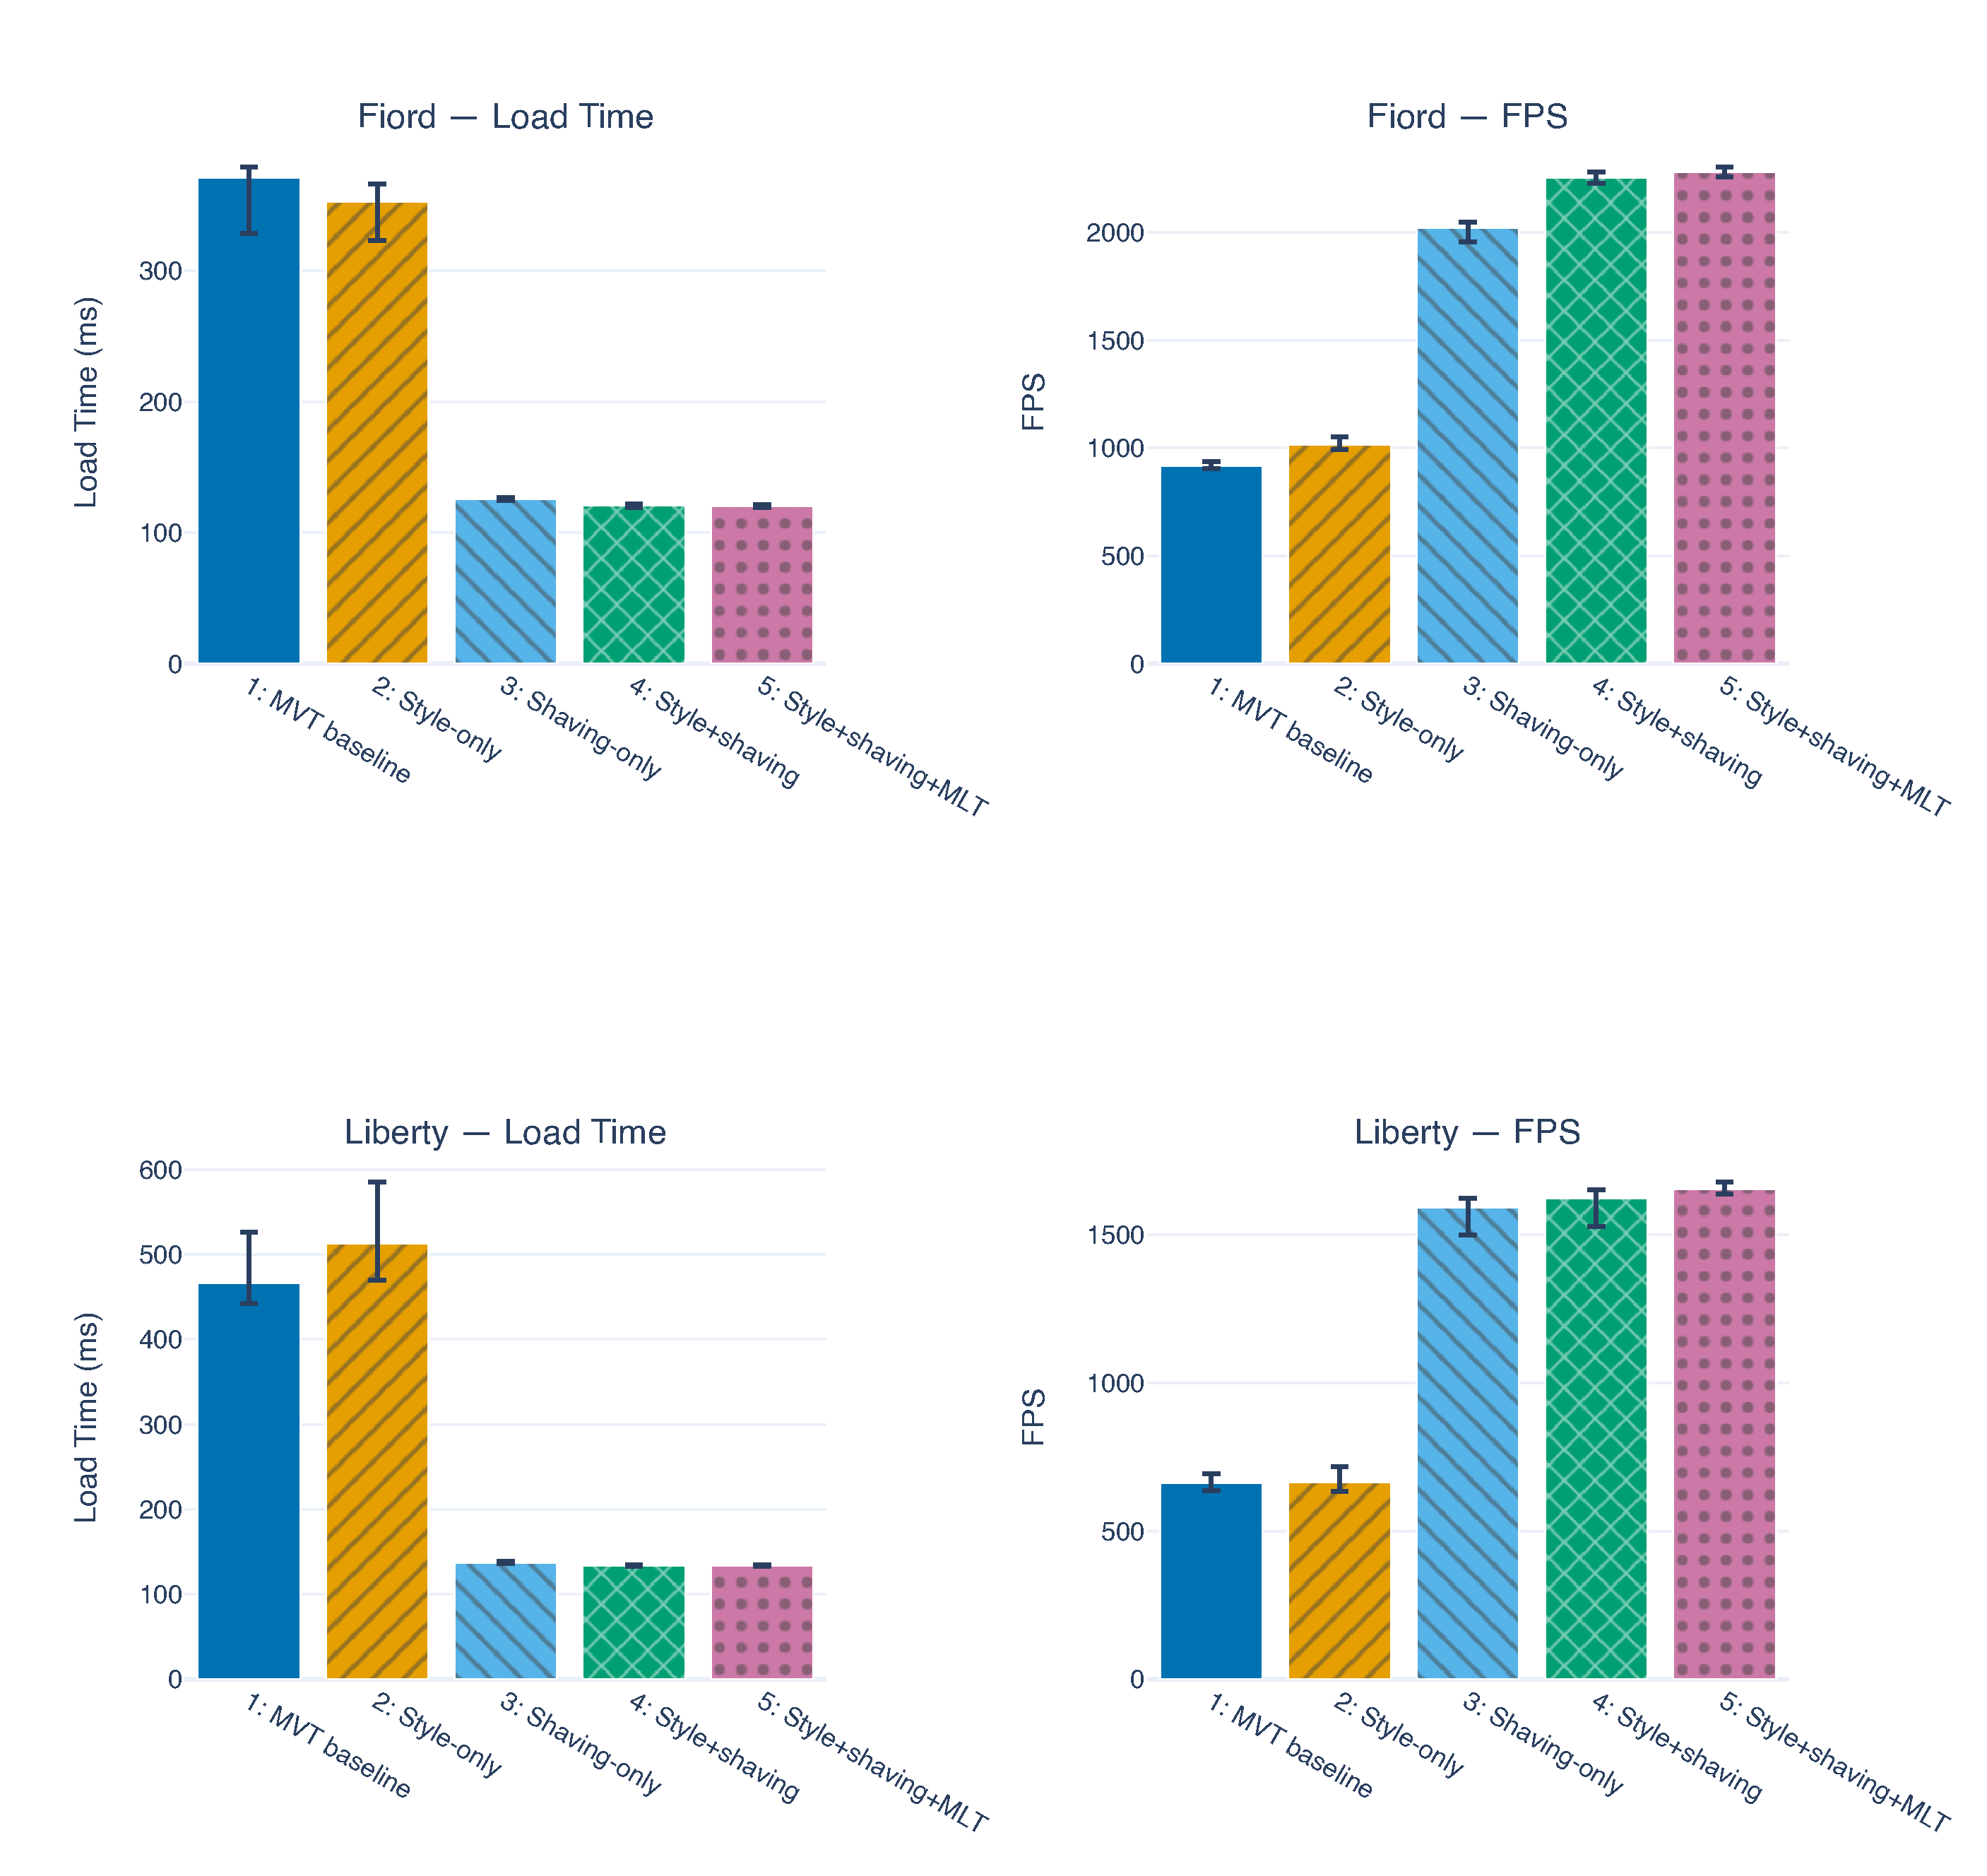
\includegraphics[width=0.9\linewidth]{figures/rendering_metrics_mlt.pdf}
    \caption{
Rendering metrics (load time, \ac{FPS}) across configurations~1-5, enabling direct comparison with Experiments~1-2 in the combined analysis.
The figure shows the significant drop in both load time and increase in \ac{FPS} for tile shaving, as well as the fact that style-only optimization is ineffective.
We also confirm the \ac{MLT} implementation to sligtly decrease performance because the current implementation still internally converts to \ac{MVT}}
    \label{fig:rendering_metrics_mlt}
\end{figure}


\subsection{Results: Encoding the Shaved Data}\label{sub:mlt_encoding_results}

Once shaving has fixed what data survives, the encoding stage determines whether those savings reach the wire.
\cref{fig:shaving_effectiveness_per_zoom} plots total tile size per zoom level for both \ac{MVT} and our \ac{MLT} encoder, with and without shaving via the Liberty advisory.
The gap between each format and its shaved counterpart quantifies the data removed by the pruning advisory.
The gap between the shaved \ac{MVT} and the shaved output of our encoder quantifies the additional contribution of columnar encoding on the already-pruned data.
Both formats benefit from shaving across all compression schemes, confirming that the advisory operates on the data itself rather than relying on format-specific redundancy.
\cref{fig:encoder_comparison} reframes the same evidence as a ratio against the \ac{MVT} baseline, adding the reference \ac{MLT} encoder of Tremmel \& Zink~\cite{tremmelMapLibreTileNext2025b} for comparison: our encoder's curves remain at roughly $0.6$-$0.8\times$ \ac{MVT} throughout the zoom range, whereas the reference-encoder curves drift above $1.0\times$ at several zoom levels under brotli/zstd, underscoring that the gains attributed to the \ac{MLT} format in this thesis come almost entirely from the encoder-side strategy competition and not from the columnar format alone.

\begin{figure}[htbp]
    \centering
    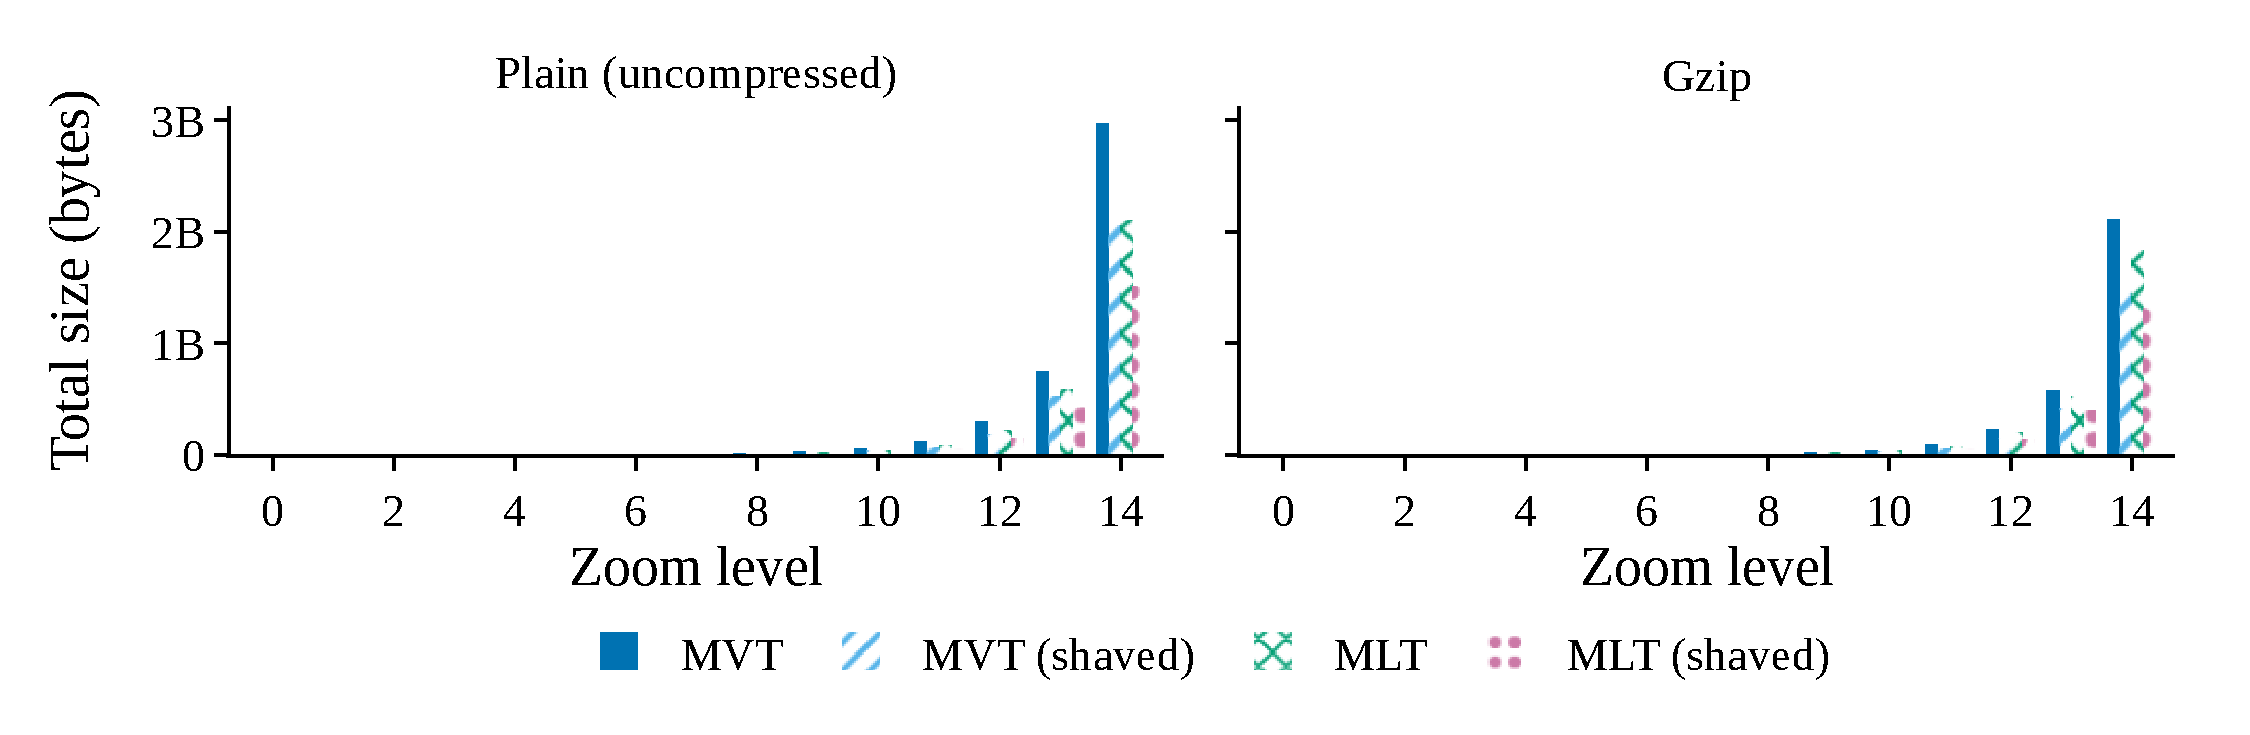
\includegraphics[width=0.9\linewidth]{figures/shaving_effectiveness_per_zoom}
    \caption{
Total tile size per zoom level for unshaved and shaved variants of
      both \ac{MVT} and our \ac{MLT} encoder, using the Liberty advisory.  The gap
      between each format and its shaved counterpart quantifies the data removed
      by the pruning advisory.
The gap between the shaved \ac{MVT} and the
      shaved output of our encoder quantifies the additional contribution of
      columnar encoding}
    \label{fig:shaving_effectiveness_per_zoom}
\end{figure}

\paragraph{Isolating the Contribution of Our Encoder's Strategy Selection}
To separate the contribution of the multi-strategy competition (this work) from that of the \ac{MLT} format as proposed by Tremmel and Zink~\cite{tremmelMapLibreTileNext2025b}, we report in \cref{fig:encoder_comparison} both a per-zoom breakdown and the total encoded size of the Germany OpenMapTiles tileset (zoom~0-14, \num{256588} tiles) under three encoders (\ac{MVT} as the row-oriented protobuf baseline, the reference \ac{MLT} encoder of Tremmel and Zink as the columnar baseline, and our \ac{MLT} encoder with sort-strategy competition, per-stream profiling, and shared-dictionary clustering) and across four wire compressions (none, gzip-9, Brotli-11, zstd-22).

\begin{figure}[htbp]
\centering
    \begin{subfigure}[t]{0.95\linewidth}
        \centering
        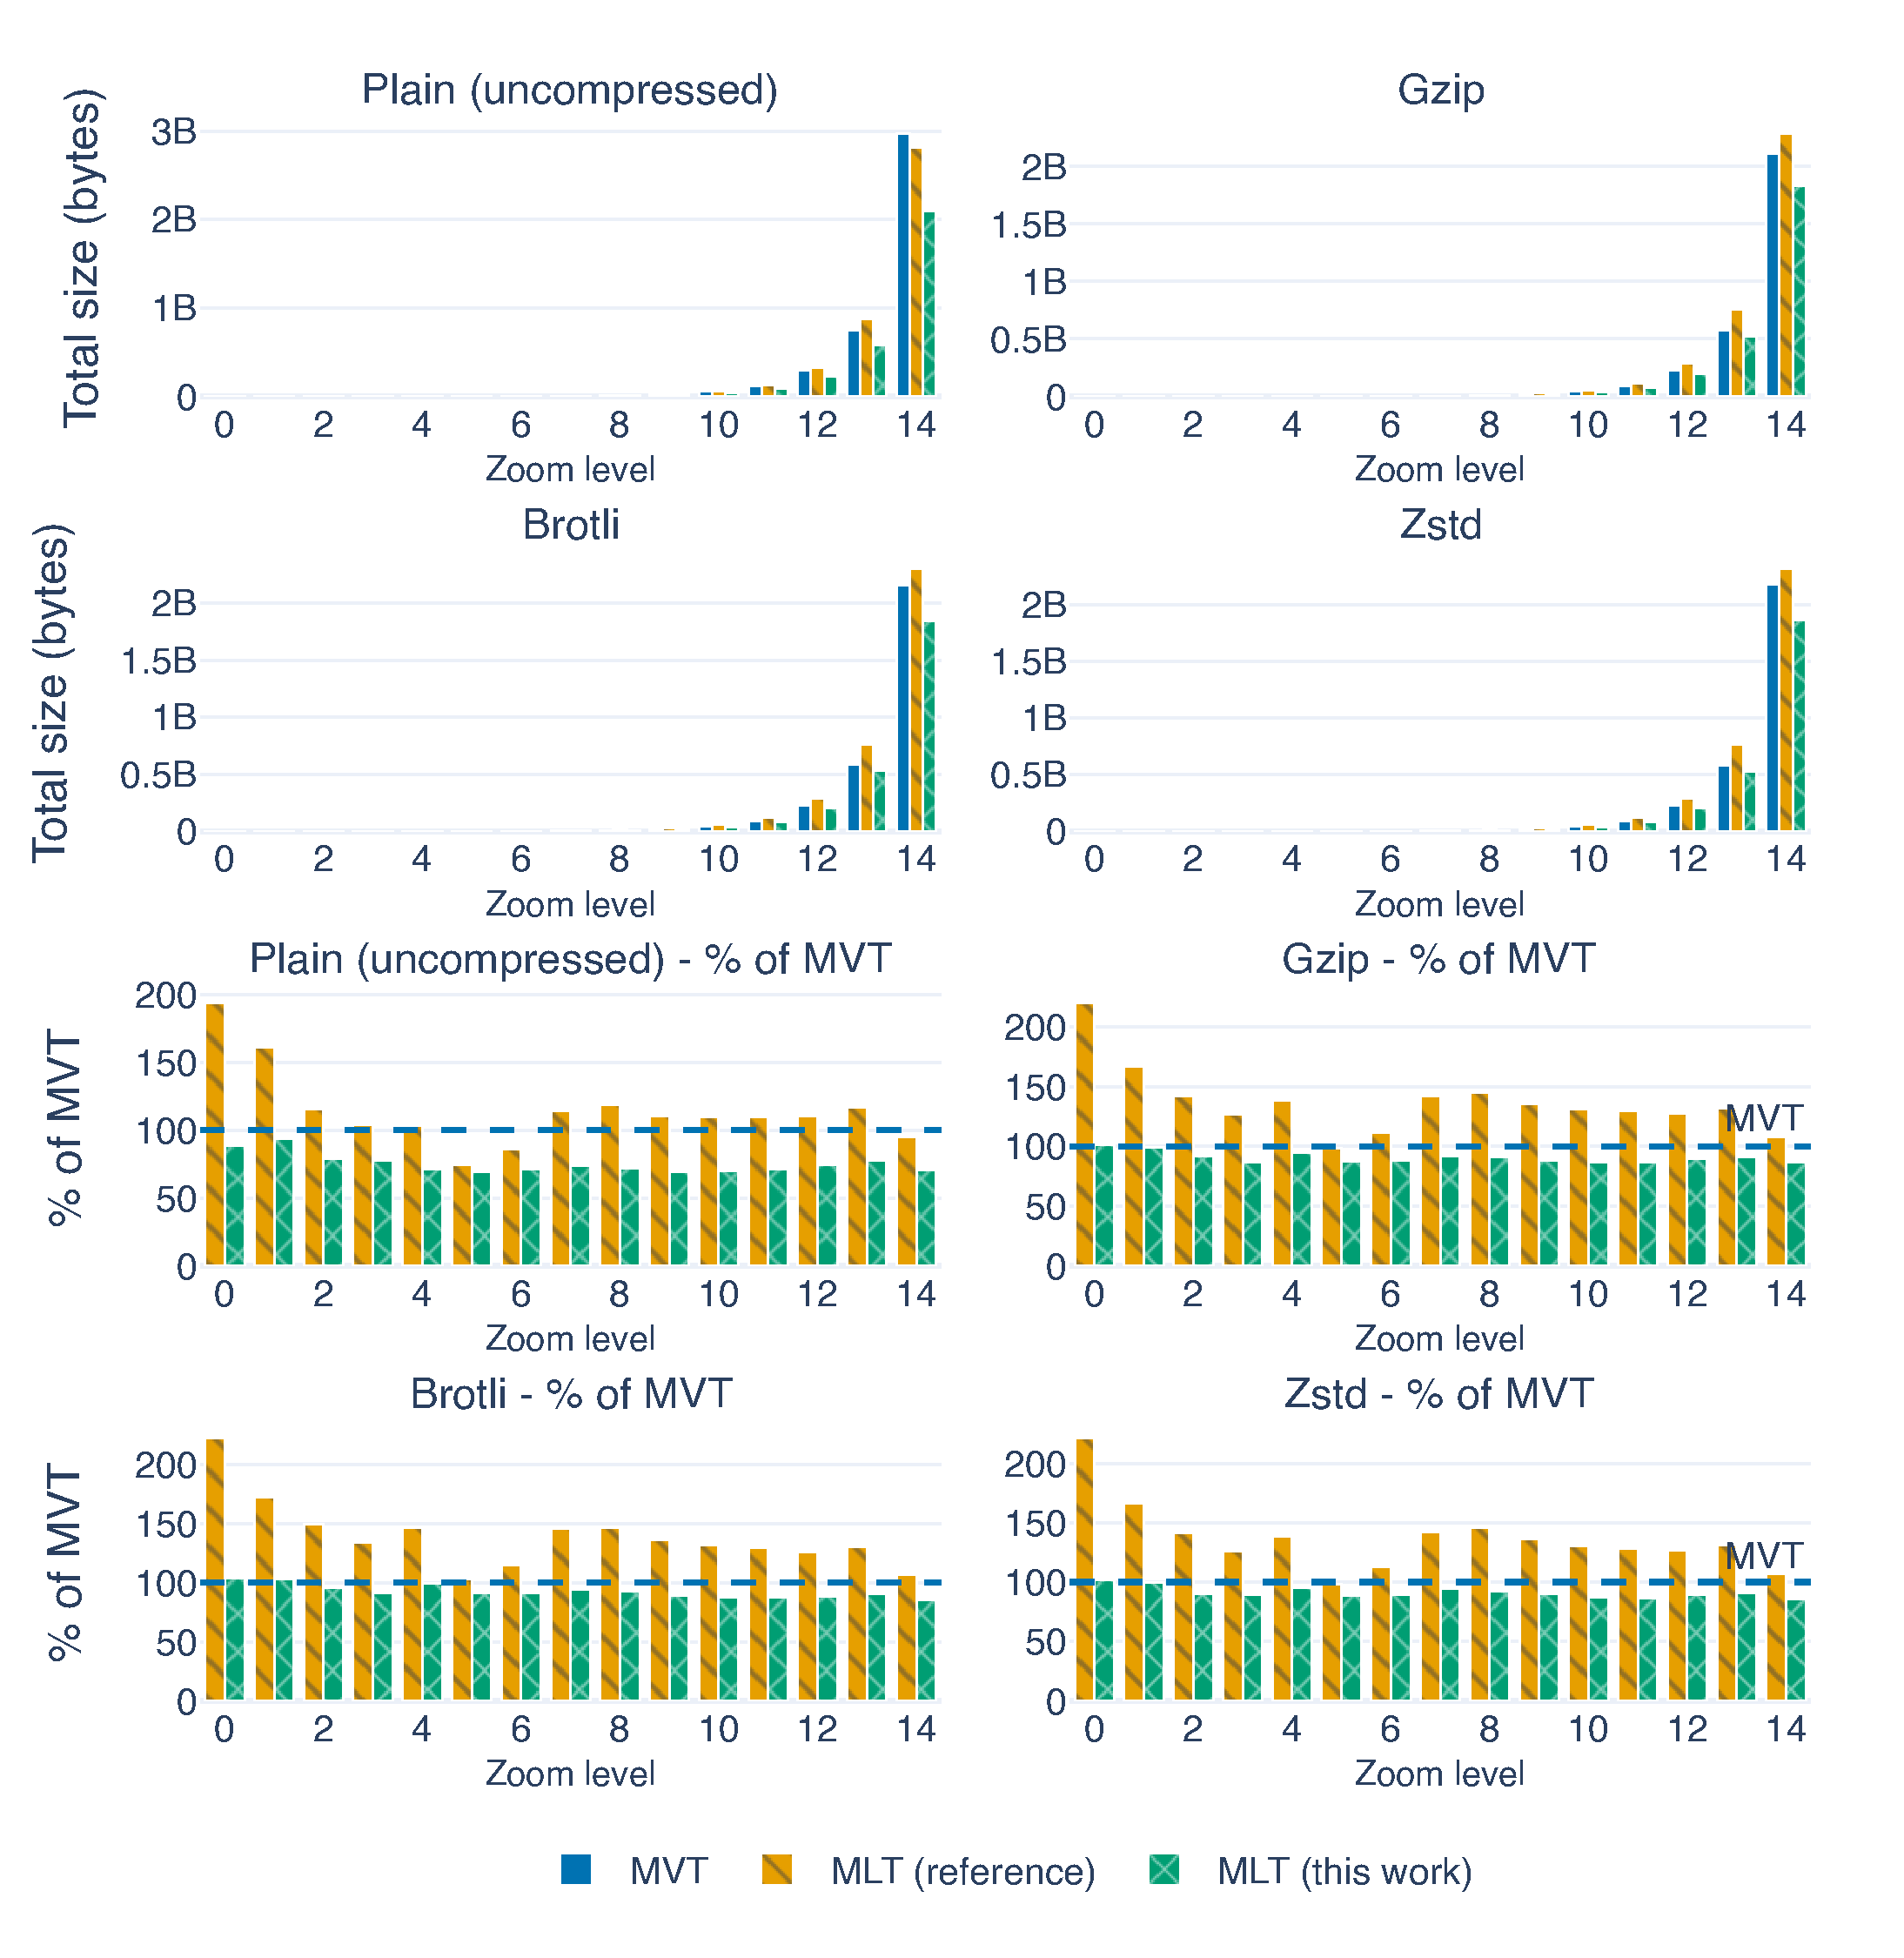
\includegraphics[width=\linewidth]{figures/encoder_comparison_per_zoom}
        \caption{
Per-zoom total tile size for the three encoders under four wire compressions}
        \label{fig:encoder_comparison_per_zoom}
    \end{subfigure}

    \vspace{1em}

    \begin{subfigure}[t]{\linewidth}
        \centering
        \begin{tblr}{colspec={l r r r r}, rows={font=\small}, row{1}={font=\small\bfseries}}
        \toprule
        Encoder & Plain (GB) & gzip (GB) & Brotli (GB) & zstd (GB) \\
        \midrule
        \ac{MVT}              & 4.24 & 3.08 & 3.13 & 3.16 \\
        \ac{MLT} (reference) & 4.26 & 3.54 & 3.57 & 3.60 \\
        \ac{MLT} (this work) & \textbf{3.06} &  \textbf{2.70} &  \textbf{2.72} &  \textbf{2.75} \\
        \midrule
        $\Delta$ ours vs.\ reference & $-28.3\%$ & $-23.8\%$ & $-23.7\%$ & $-23.6\%$ \\
        $\Delta$ ours vs.\ \ac{MVT}  & $-27.9\%$ & $-12.3\%$ & $-13.1\%$ & $-12.9\%$ \\
        \bottomrule
        \end{tblr}
        \caption{
Total tileset size for the three encoders under four wire compressions.
          The \ac{MLT} (reference) column reports the baseline from~\cite{tremmelMapLibreTileNext2025b}, updated with encoding improvements backported from our encoder's development (correct delta-zigzag sequencing, \ac{RLE} viability checks, \ac{FSST} thresholds).
          The \ac{MLT} (this work) column reports the encoder developed in this thesis}
        \label{tab:mvt_mlt_comparison}
    \end{subfigure}
\caption[Encoder comparison: per-zoom breakdown and total tileset size]{Encoder comparison for the Germany OpenMapTiles tileset (zoom~0-14, \num{256588} tiles).
Our \ac{MLT} encoder achieves \qty{28.3}{\percent} smaller total size than the reference baseline under no wire compression.
The reference encoder drifts above \ac{MVT} size at several zoom levels under Brotli/zstd, whereas our encoder remains below \ac{MVT} throughout.}
\label{fig:encoder_comparison}
\end{figure}

The headline is the \qty{28.3}{\percent} reduction our encoder achieves over the reference baseline under no wire compression.
The reference baseline already incorporates encoding fixes backported from our encoder's development (correct delta-zigzag sequencing, \ac{RLE} viability checks, \ac{FSST} thresholds), so the \qty{28}{\percent} isolates the contribution of automatic strategy selection over a correctly-implemented fixed-plan encoder rather than conflating bug fixes with the innovation we want to attribute to.

The finding in the table that is easiest to overlook, and the one we found most uncomfortable when we first plotted it, is that the reference baseline is \emph{worse} than gzip-compressed \ac{MVT} (\qty{3.54}{\giga\byte} vs.\ \qty{3.08}{\giga\byte}).
General-purpose LZ77-family compressors already exploit most of the row-level redundancy in the protobuf wire format, and a columnar encoder that uses fixed per-column schemes cannot keep up.
The data-driven strategy selection in our encoder reclaims this gap and goes past it: our encoder under gzip is \qty{12.3}{\percent} smaller than \ac{MVT} under gzip, and the advantage holds (\qty{12.9}{\percent}) even against zstd-22, the strongest general-purpose compressor in the comparison.

The relative gap between our encoder and the reference is roughly constant across all four compressors (\qty{-23}{\percent} to \qty{-28}{\percent}).
This stability is consistent with the profiler capturing genuine redundancy that general-purpose compressors miss, but it could equally reflect that the profiler removes the same redundancy the compressors would have.
The cleaner evidence for the profiler's value is the absolute comparison: our encoder, uncompressed (\qty{3.06}{\giga\byte}), is already smaller than \ac{MVT}+gzip (\qty{3.08}{\giga\byte}), confirming that per-stream encoding captures type-specific redundancy that LZ77-family compressors miss on the interleaved protobuf byte stream.
This directly answers the question we posed at the start of \cref{sec:exp_mlt}: our encoder's contribution lives in the joint strategy-selection layer that sits on top of the columnar format, not in the format alone.

\paragraph{Scope of the Encoder Contribution}
We measured the \qty{28}{\percent} reduction reported in \cref{tab:mvt_mlt_comparison} on the \emph{unshaved} Germany tileset, so it is an encoder-only improvement, independent of the style-driven optimizations.
It reflects the combined effect of sort-strategy competition, per-stream profiling, and shared-dictionary clustering.
These three mechanisms are tightly coupled (sort order affects column distributions, which affect profiling decisions), so a per-mechanism decomposition is not feasible without re-engineering the encoder.
This result is complementary to, but separate from, the style-data bridge: style-driven tile shaving reduces tile content before encoding, while the encoder improvements reduce the encoded size of whatever content remains.
The two contributions stack (shaved tiles encoded with our encoder are smaller than shaved tiles encoded with the reference baseline), but they address orthogonal sources of redundancy.

\paragraph{zstd-on-\acs{MVT} Comparison}
A natural objection is that general-purpose compressors such as zstd-22 or Brotli-11 should be sufficient: if compression is the goal, simply applying the strongest available compressor to the existing \ac{MVT} wire format would avoid the complexity of a columnar encoder entirely.
\Cref{tab:mvt_mlt_comparison} answers this directly.
\ac{MVT} under zstd-22 yields \qty{3.16}{\giga\byte} for the Germany tileset, whereas our encoder under the same compressor yields \qty{2.75}{\giga\byte}, a \qty{12.9}{\percent} reduction.
We attribute this to a structural difference: a general-purpose compressor sees the interleaved, heterogeneous protobuf byte stream and must discover redundancy across mixed data types.
A columnar encoder, by contrast, groups homogeneous values (all road classes in one stream, all vertex deltas in another) and each stream compresses more effectively under lightweight per-type codecs (delta-\acs{RLE} for monotonic integers, dictionary encoding for low-cardinality strings, \ac{FSST} for high-cardinality strings) than a monolithic LZ77-family compressor can achieve on the interleaved byte stream.
The columnar advantage is preserved \emph{after} applying the same general-purpose compressor on top: the per-column codecs have already removed most of the type-specific redundancy, so the post-hoc compressor has less work to do but starts from a lower baseline.
This finding is consistent with the columnar-database literature, where per-column lightweight encoding consistently outperforms row-level block compression even when the block compressor is state-of-the-art~\cite{kuschewskiBtrBlocksEfficientColumnar2023}.

\paragraph{Decoder Cost}
A legitimate concern for any multi-encoding scheme is that the client must pay the decoder cost, which can erode the transfer savings on mobile or battery-constrained targets.
We engineered the decoder to amortise its per-column dispatch over per-feature work (\cref{sub:encoding_strategies}).
Empirically, our benchmarks on the full Germany tileset show end-to-end rendering metrics comparable to or better than \ac{MVT} at matched workloads, and we see no negative effect in the sustained frame-time metrics of \cref{sub:combined_marginal}.


\paragraph{Decoding Throughput}
To isolate decoding latency from the browser-based rendering benchmark (where it is embedded in \texttt{loadMs}), we use Criterion micro-benchmarks to measure full-decode throughput for our \ac{MLT} decoder vs.\ \ac{MVT} with and without transport compression.
Each benchmark parses the tile header and materialises all features and properties; \ac{MVT} variants include gzip decompression in the measured path.
\Cref{tab:decode_throughput} reports the results on a representative subset of the OpenMapTiles fixture tiles at zoom levels~4, 7, and~13 (100~samples per cell).

\begin{table}[htbp]
\centering
\small
\begin{tblr}{colspec={l r r r}, rows={font=\small}, row{1}={font=\small\bfseries}}
\toprule
Format & Zoom~4 & Zoom~7 & Zoom~13 \\
\midrule
\ac{MLT} (this work) & \qty{5.73}{\milli\second} & \qty{19.4}{\milli\second} & \qty{4.09}{\milli\second} \\
\ac{MVT}+gzip & \qty{47.6}{\milli\second} & \qty{103}{\milli\second} & \qty{18.7}{\milli\second} \\
\ac{MVT} (uncompressed) & \qty{44.2}{\milli\second} & \qty{90.6}{\milli\second} & \qty{16.5}{\milli\second} \\
\midrule
Speedup (vs.\ gzip) & $8.3\times$ & $5.3\times$ & $4.6\times$ \\
\bottomrule
\end{tblr}
\caption{
Full-decode latency for our \ac{MLT} decoder vs.\ \ac{MVT} on OpenMapTiles fixture tiles, measured by Criterion micro-benchmarks (100~samples per cell).
Our decoder achieves \numrange{96}{134}\,MiB/s decode throughput vs.\ \numrange{15}{23}\,MiB/s for \ac{MVT}+gzip (measured over wire-format input size)}
\label{tab:decode_throughput}
\end{table}

The \ac{MLT} decoder's columnar layout enables selective column access and avoids the per-feature tag-parsing overhead of protobuf, which accounts for the speedup even before transport decompression is considered: our decoder is $4.0$-$7.7\times$ faster than uncompressed \ac{MVT}.
These micro-benchmark results complement the browser-based \texttt{loadMs} metric by providing an isolated measurement of the decoding-latency axis of Research Goal~R3, even though they are not 1:1 applicable because we do not use our decoder in \texttt{maplibre-gl-js}.

\subsection{Discussion}\label{sub:mlt_discussion}

Tile shaving alone cuts pooled median load time by \qty{71.5}{\percent} and lifts \ac{FPS} by \qty{184}{\percent}, while style-only passes contribute \qty{-4.1}{\percent} on load.
The two channels compose additively, not synergistically.
We discuss why the channels stay additive, the cache-fragmentation trade-off that style-dependent tiles create on shared \acsp{CDN}, and the geometry-simplification axis we leave out of scope.

\paragraph{Dominance of Tile Shaving and Additive Style-Pass Contribution}
The headline finding of this experiment is that tile shaving is the dominant contributor to load-time and transfer-size improvements, while style-level passes provide a modest, additive assist.
Dead layer elimination (Experiment~2) removes style layers whose filters are unsatisfiable.
Each removed layer reduces the set of referenced properties in the pruning advisory, which in turn can eliminate columns from the encoded tile.
Metadata refinement tightens zoom bounds, which causes the advisory to mark additional zoom levels as unused, potentially eliminating tiles entirely.
However, the aggregate data shows no super-additive interaction at the median level (\cref{sub:mlt_results}): the combined style+shaving reduction is approximately the sum of the individual reductions, not greater.
We therefore best understand the style-level passes as useful enablers (simplifying the advisory and improving code quality) rather than as co-equal partners in a synergistic cascade.
The encoding stage that follows benefits from this enabling effect: shaved data presents longer runs and smaller dictionaries to the per-stream profiler, which is why we place the multi-strategy competition in the same pipeline rather than as a standalone encoder paper.

\paragraph{Style-Dependent Tile Sizes}
A consequence of style-driven shaving is that different styles produce different tile sizes from the same source data.
To quantify this variation, we ran the full shaving pipeline (optimize with all passes, generate pruning advisory, apply advisory as \ac{MVT}) on the same Germany tileset (\qty{3.07}{\giga\byte}, OpenMapTiles schema, zoom levels 0-14) for each of the 11 \ac{OMT}-compatible styles in the benchmark corpus.
\cref{fig:tile_shave_per_style} shows the results: tile-data reductions range from \qty{19.8}{\percent} (Bright) to \qty{46.3}{\percent} (Toner), with a median of \qty{29.0}{\percent}.
Styles that reference fewer source-layers and property columns (such as Toner with monochrome road/water/boundary only and Americana focused on shield and label rendering) leave more tile data unused, enabling the advisory to strip more columns and features.
Conversely, broad-coverage styles like Bright and OSM~Bright reference most of the tileset's property columns, limiting the shaving headroom.
We see this observation as highlighting a fundamental trade-off: there is no single optimal tile.
The optimal encoding depends on the rendering style, which is a design choice.

\begin{figure}[htbp]
    \centering
    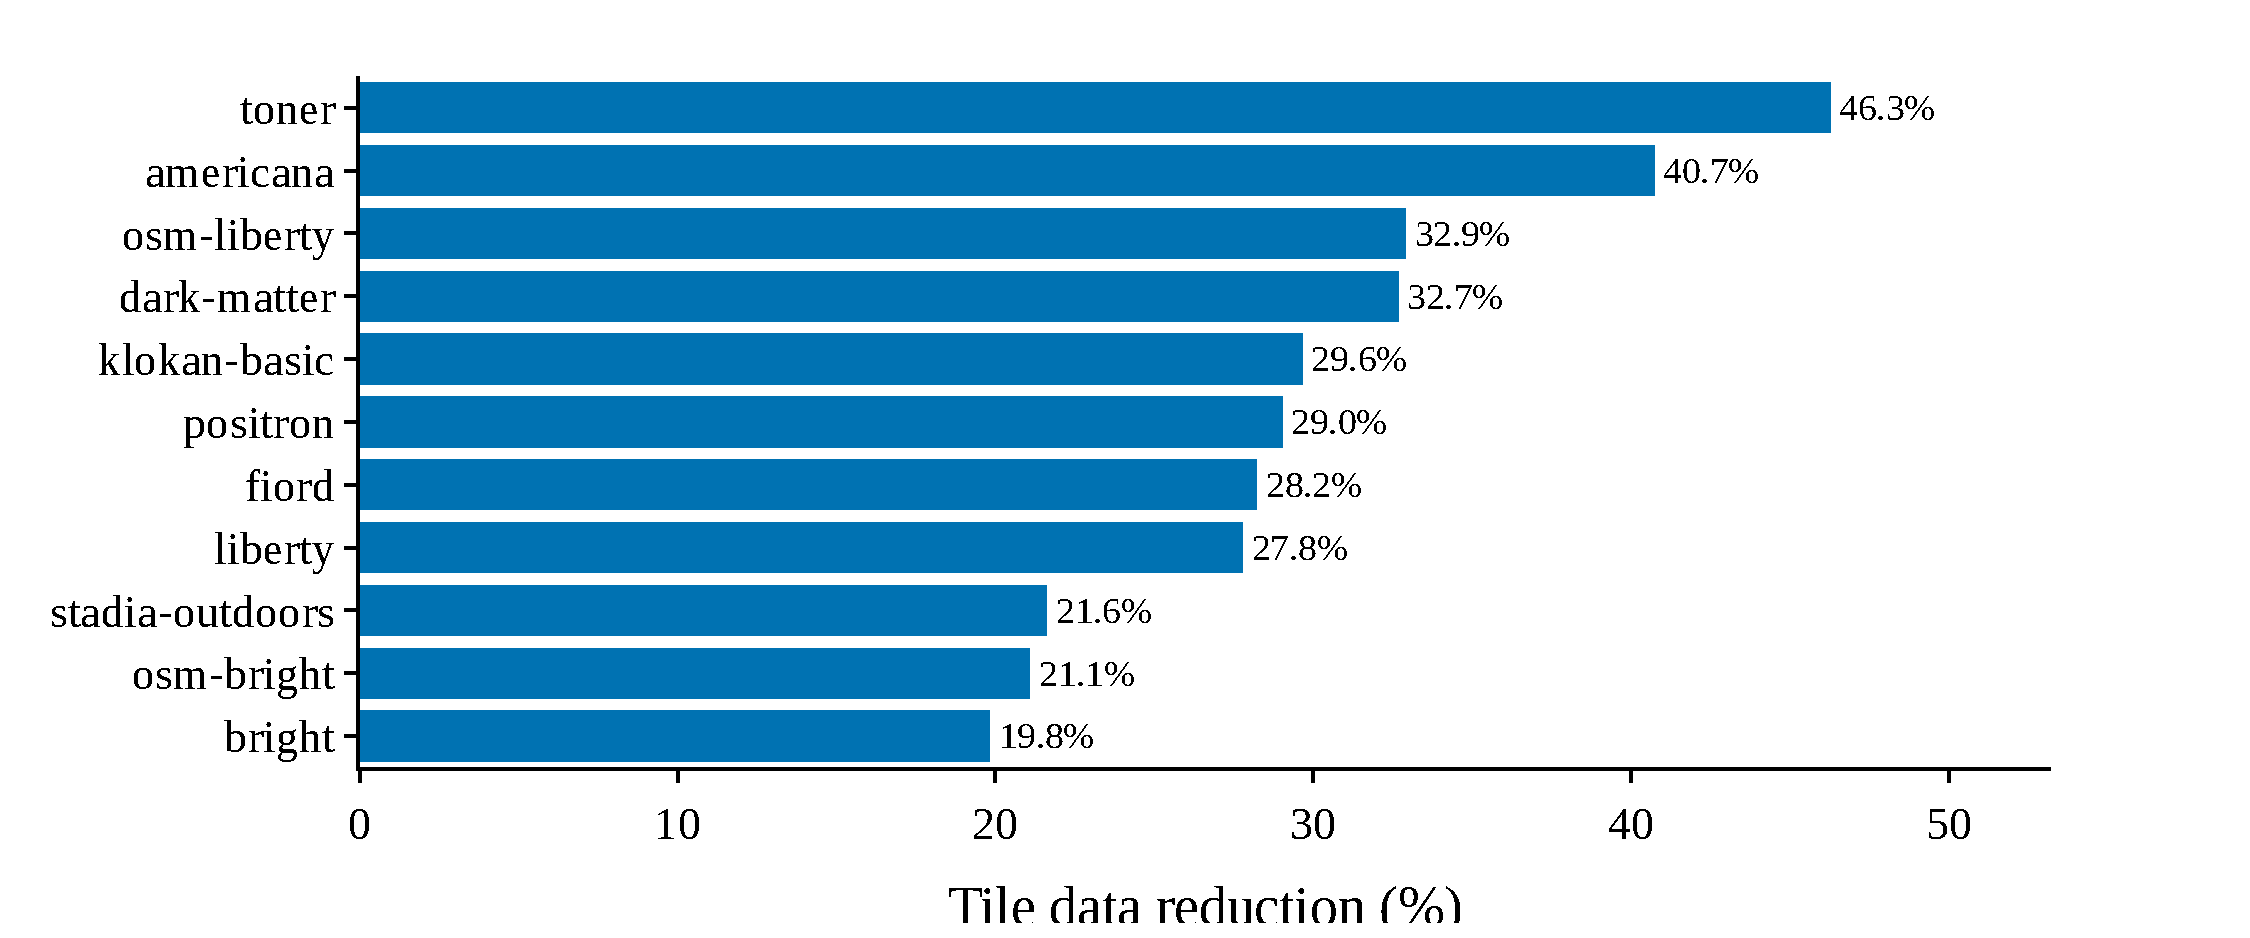
\includegraphics[width=0.8\linewidth]{figures/tile_shave_per_style}
    \caption{
On-Wire data reduction from style-driven \ac{MVT} shaving across 11 \ac{OMT}-compatible styles, applied to the same \qty{3.07}{\giga\byte} Germany tileset.  Styles that reference fewer source-layers and properties achieve larger reductions}
    \label{fig:tile_shave_per_style}
\end{figure}

\paragraph{Cache Fragmentation Trade-Off}
A direct operational consequence of style-dependent tiles is that shared \ac{CDN} caching is partially defeated.
Two styles that served identical tiles under \ac{MVT} now fetch distinct shaved variants, and a \ac{CDN} must either key its cache on (tile, style) pairs or accept that a hit on one style is a miss on another.
For deployments where a single style dominates traffic, style-driven shaving is strictly beneficial.
For multi-tenant tile servers hosting dozens of styles, operators should apply shaving per style and cache the resulting tile variants independently (the approach of Mapbox's closed-source \enquote{style-optimized vector tiles} service~\cite{StyleoptimizedVectorTiles}).

We frame the decision with a per-style break-even model.
A vector-tile source's \texttt{encoding} field selects \ac{MVT} or \ac{MLT}, so the two formats cannot mix within one source.
Unshaved \ac{MLT} is possible in principle but not emitted by our tool, so each style is served either as shaved \ac{MLT} (with its own \emph{(tile, style)} cache-key namespace) or as raw \ac{MVT} (sharing cache slots with all other \ac{MVT}-served styles).
The choice is usually binary per style (given most styles only have one vector tile source), and the operational question is which styles belong in which group.

Let $r$ denote the per-tile rendering-time saving from shaving (load-time reduction divided by the number of fetched tiles), $C_f$ the origin fetch cost per cache miss, $\lambda_i$ the aggregate request rate to style $i$, $N$ the number of distinct tiles, and $\mathcal{M}$ the subset of styles served as \ac{MVT} with pooled rate $\Lambda_\mathcal{M} = \sum_{i \in \mathcal{M}} \lambda_i$.
Let $h(\mu)$ denote the steady-state hit rate of a cache slot accessed at rate $\mu$ on the shared edge cache.
Under \ac{LRU}, $h$ is monotonically increasing in $\mu$ and saturates near $1$ for popular content.
A style-$j \in \mathcal{M}$ request hits the per-tile pooled slot at rate $\Lambda_\mathcal{M}/N$, while a style served as shaved \ac{MLT} hits its own \emph{(tile, style)} slot at rate only $\lambda_i/N$.
Moving style $i$ from $\mathcal{M}$ to the \ac{MLT}-served set is net-beneficial when
\[
    r \;>\; \big[\, h(\Lambda_\mathcal{M}/N) - h(\lambda_i/N) \,\big] \cdot C_f
\]
where the bracketed \emph{hit-rate gap} measures the cache warmth that style $i$ surrenders by leaving the pool.
The decision depends on style $i$'s share of pool traffic, not on the total number of styles served.

We identify two practically meaningful regimes.
A \emph{dominant style} ($\lambda_i$ comparable to $\Lambda_\mathcal{M}$) sees a near-zero gap, since the pool was already warmed almost entirely by its own traffic, and any positive $r$ justifies shaving.
A \emph{long-tail style} ($\lambda_i \ll \Lambda_\mathcal{M}$) sees a gap that approaches the full pooled hit rate $h(\Lambda_\mathcal{M}/N)$, because its private cache cannot self-warm on its own thin traffic and reverts to near-cold-start behavior.
With our benchmark values ($r \approx \qty{3}{\milli\second}$ per tile, $C_f \approx \qty{25.8}{\milli\second}$ under the Rusan et al.~\cite{rusanAssessmentPacketLatency2015} $\frac{\text{tile size}}{\qty{30}{\mega\bit\per\second}} + \frac{\qty{25}{\milli\second}}{2}$ server-side-throttle for a \qty{50}{\kilo\byte} average tile) and a representative pooled hit rate $h(\Lambda_\mathcal{M}/N) \approx 0.9$ for popular tile content, the maximum tolerable hit-rate gap is $r/C_f \approx 11.6\%$.

Under typical \ac{LRU} dynamics this in turn requires the style to hold a majority share of pool traffic before it can be shaved profitably.
We draw the corollary of the hybrid pattern from this:
shave the one or two canonical styles that dominate the pool, and leave the long tail on raw \ac{MVT}.
Traffic concentration drives this recommendation, not style count.
A server hosting fifty styles with one \qty{70}{\percent}-share dominant style behaves the same as one hosting five with the same concentration.
Our model omits spatial locality and the second-order effect that peeling the dominant style off the pool cools the cache further for the remaining \ac{MVT}-served styles, both of which would only sharpen the recommendation.

\paragraph{Geometry Simplification as out of scope}
A complementary direction we do not explore in this thesis is geometry-level pruning - coordinate precision reduction, Visvalingam~\cite{visvalingamLineGeneralisationRepeated1993} or Douglas-Peucker~\cite{douglasALGORITHMSREDUCTIONNUMBER1973} simplification, and polygon topology coalescing - which is the principal lever used by upstream generators such as Tippecanoe\footnote{\url{https://github.com/felt/tippecanoe}, last accessed 2026-04-21} and Planetiler\footnote{\url{https://github.com/onthegomap/planetiler}, last accessed 2026-04-21}.
These techniques typically deliver larger absolute savings than attribute-column pruning, but they interact non-trivially with style-defined visual thresholds (line width, dash pattern length, label anchor placement) and would violate the pixel-identity soundness criterion established in \cref{sec:problem_statement}.
Style-driven geometry simplification, choosing a simplification tolerance that is demonstrably below the smallest visible feature at each zoom level, is an interesting direction for future work but we do not pursue it here.
We therefore quantify the size reductions achievable \emph{without} touching geometry at all, which understates the total optimizations headroom a production pipeline could reach by composing this work with an upstream simplifier.

\section{Cross-Style Generalisation}\label{sec:exp_cross_style}
\begin{keytakeaways}
\item Static-only passes generalize: median \qty{31.4}{\percent} raw reduction across 13 unseen styles, none regressed.
\item Initial style size and complexity does not predict reduction ($r = 0.35$, $n = 13$, $p = 0.24$).
\item These numbers are a lower bound.
Stats-driven and data-level passes were not applied here.
\end{keytakeaways}

\noindent In the preceding experiments we evaluated optimizations effectiveness on the curated benchmarking corpus of 15 styles described in \cref{sub:deep_corpus}.
To assess whether the observed gains generalize, we apply the optimizer to the 13~styles of the Maputnik generalization corpus introduced in \cref{sub:generalization_corpus}.
We use three tiers of breadth because end-to-end rendering benchmarks require tile data and browser automation infrastructure that does not scale to all styles: we benchmark ten deep-corpus styles end-to-end with tile data, eleven \ac{OMT}-compatible styles at the tile-shaving size level, and evaluate thirteen additional styles with static analysis only.

\subsection{Methodology}\label{sub:cross_methodology}

We use static analysis only for the cross-style evaluation: we optimize each style with all passes enabled, and compare the resulting style to the original on size and complexity metrics.
We execute no rendering benchmarks, as the diverse styles reference incompatible tile schemas and tile sources that we cannot uniformly provision.

\subsection{Results}\label{sub:cross_results}

\cref{fig:cross_style_reduction} shows per-style percentage reductions (raw, gzip, Brotli) across the 13 Maputnik styles, sorted by raw reduction.
The key question here is whether the distribution clusters tightly around the deep corpus median or fans out with substantial per-style variance.
\cref{fig:cross_style_complexity_scatter} then plots each style's initial complexity against its achievable reduction, testing the hypothesis that verbose institutional styles (the right-hand side of the scatter) have disproportionately more optimizations headroom than already-compact minimal basemaps on the left.

The distribution fans out considerably:
raw reductions range from \qty{3.2}{\percent} (Stadia Outdoors) to \qty{67.7}{\percent} (LocationIQ Streets), with no style regressing.
Under gzip compression the range narrows to \qtyrange{3.9}{22.4}{\percent} (median \qty{11.4}{\percent}), confirming that some of the raw-byte savings overlap with what gzip already captures.
The top reducers (LocationIQ Streets at \qty{67.7}{\percent} raw, Americana at \qty{59.2}{\percent}, and MapTiler Toner at \qty{57.5}{\percent}) are styles with either verbose filter logic (LocationIQ, Americana) or highly repetitive property structures (Toner).
At the low end, Stadia Outdoors (\qty{3.2}{\percent}) and the two AWS styles (both at \qty{10.6}{\percent}) leave little for the optimizer to remove: the AWS pair shares a codebase of hand-tuned expressions with few redundancies, while Stadia Outdoors is a compact, already-minified basemap.
We observe no statistically significant correlation between initial \ac{AST} node count and reduction ($r = 0.35$, $n = 13$, $p = 0.24$).
The sample size is too small for this correlation to be meaningful.  Americana has by far the highest initial complexity (\num{48510} nodes) and is also one of the top three reducers, but it is a single high-leverage point: dropping it flips the sign to $r = -0.54$, underscoring that no stable trend exists at this sample size.

\begin{figure}[htbp]
    \centering
    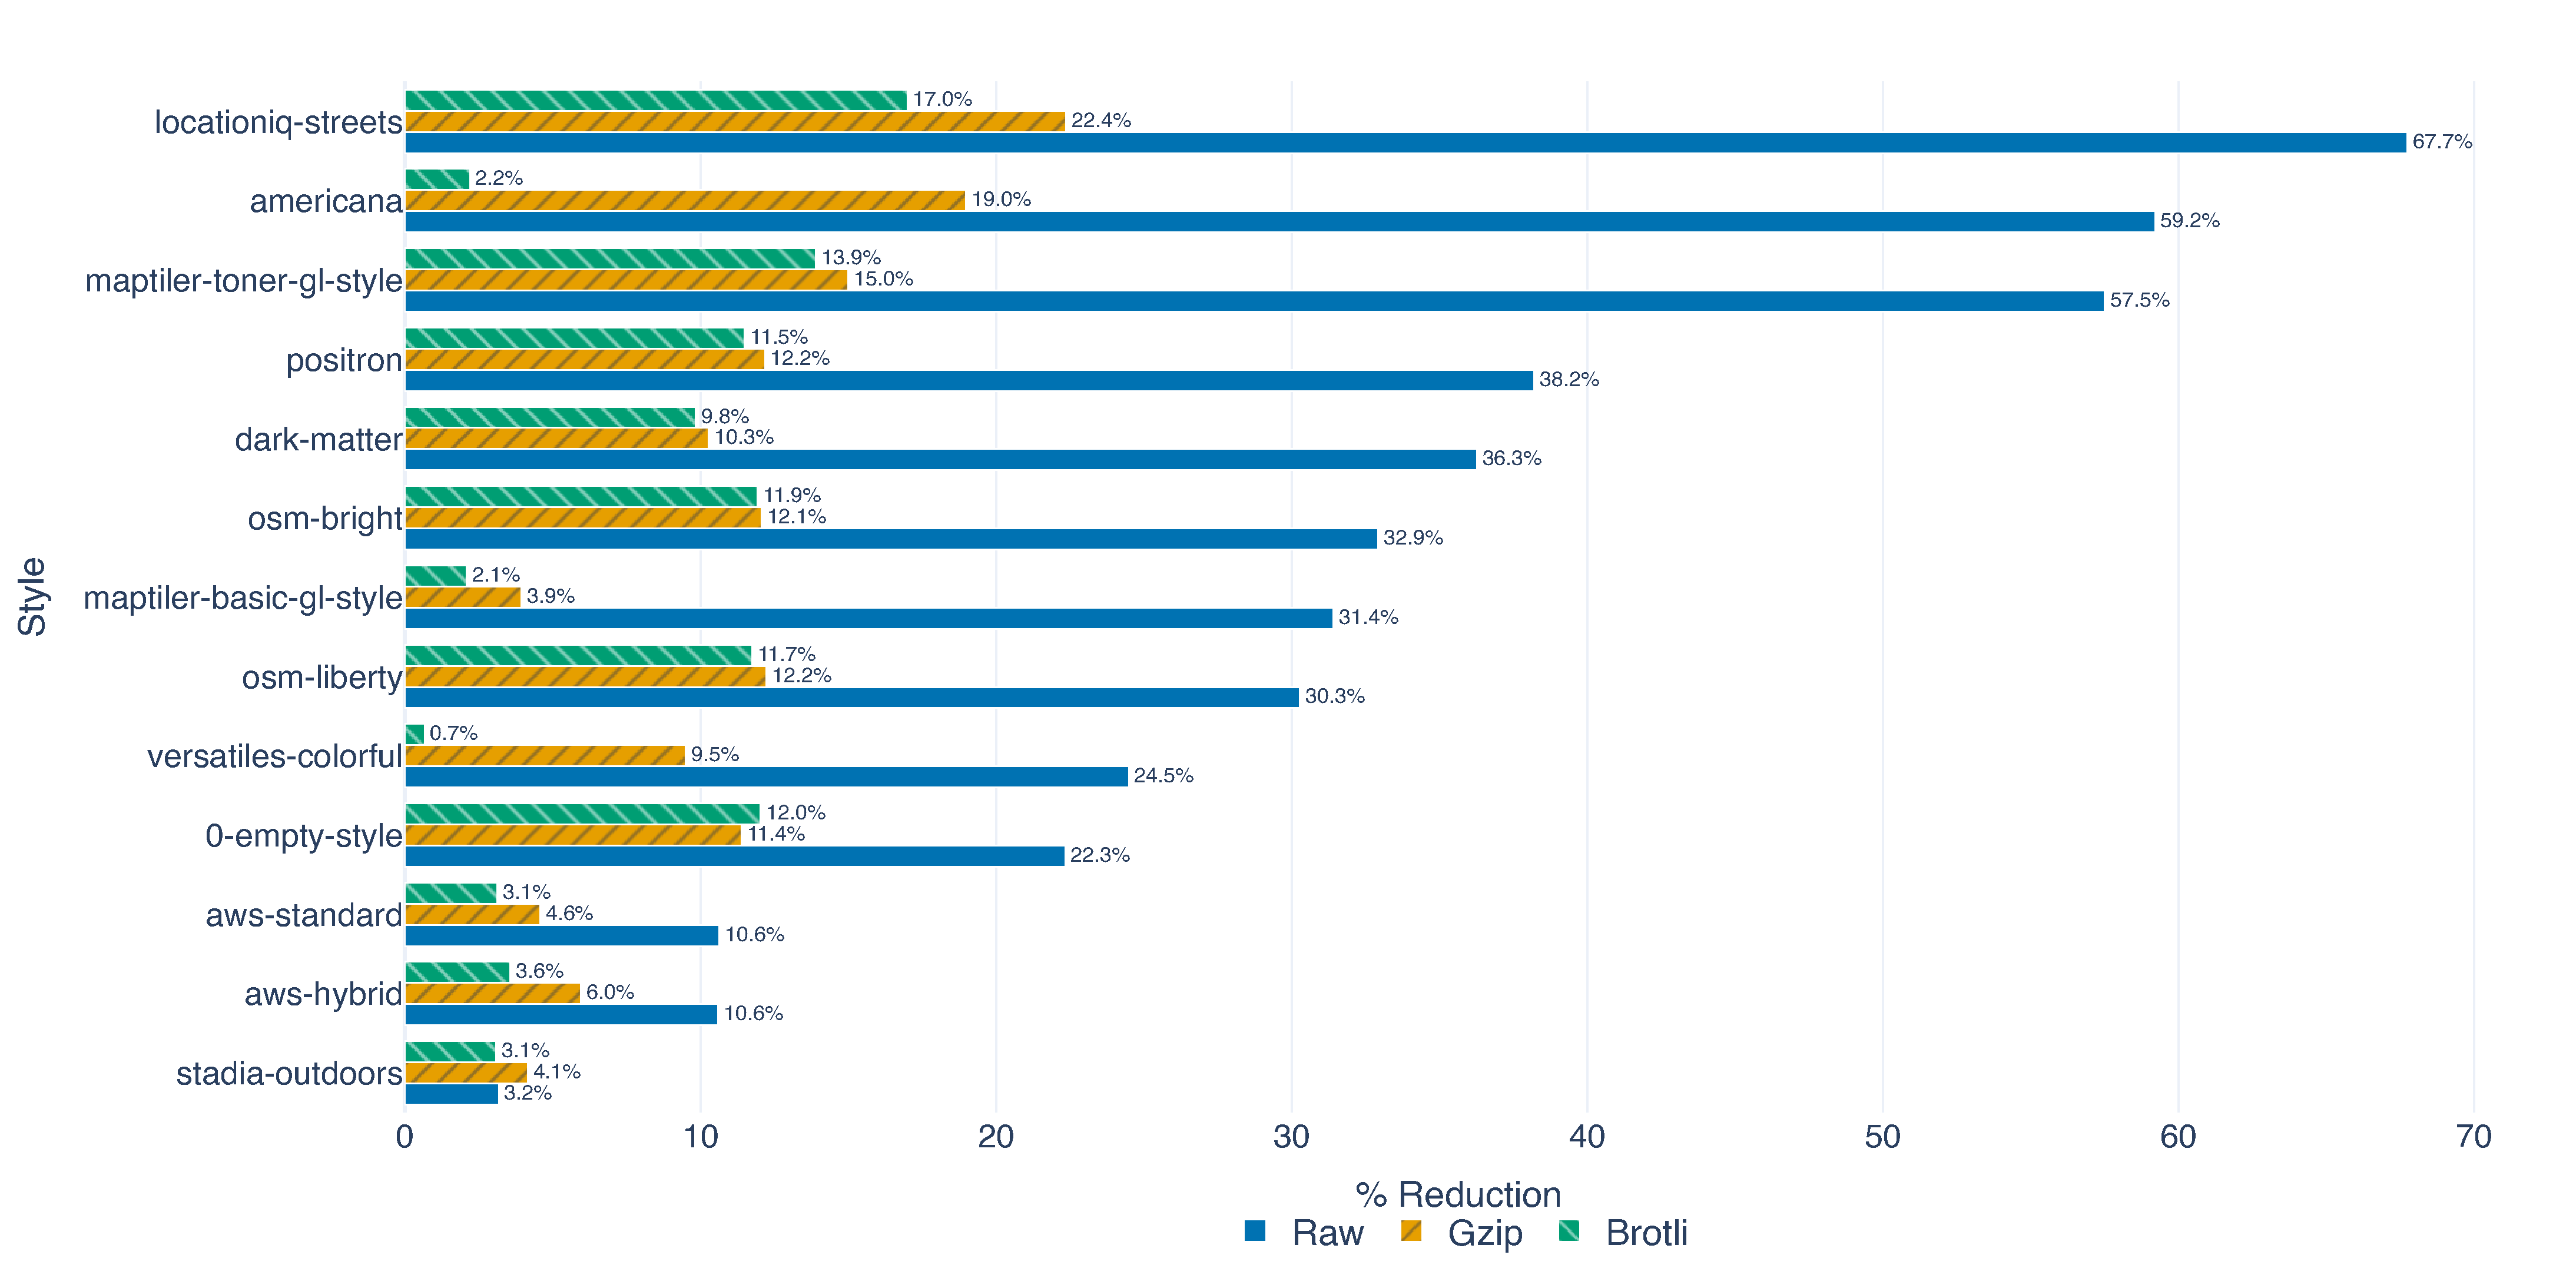
\includegraphics[width=\linewidth]{figures/cross_style_reduction.pdf}
    \caption{
Per-style percentage reduction in style size (raw, gzip, Brotli) across the Maputnik generalization corpus, with styles sorted by raw reduction.
Raw reductions range from \qty{3.2}{\percent} to \qty{67.7}{\percent}, confirming that automatic optimization yields meaningful gains across styles regardless of origin.}
    \label{fig:cross_style_reduction}
\end{figure}

\begin{figure}[htbp]
    \centering
    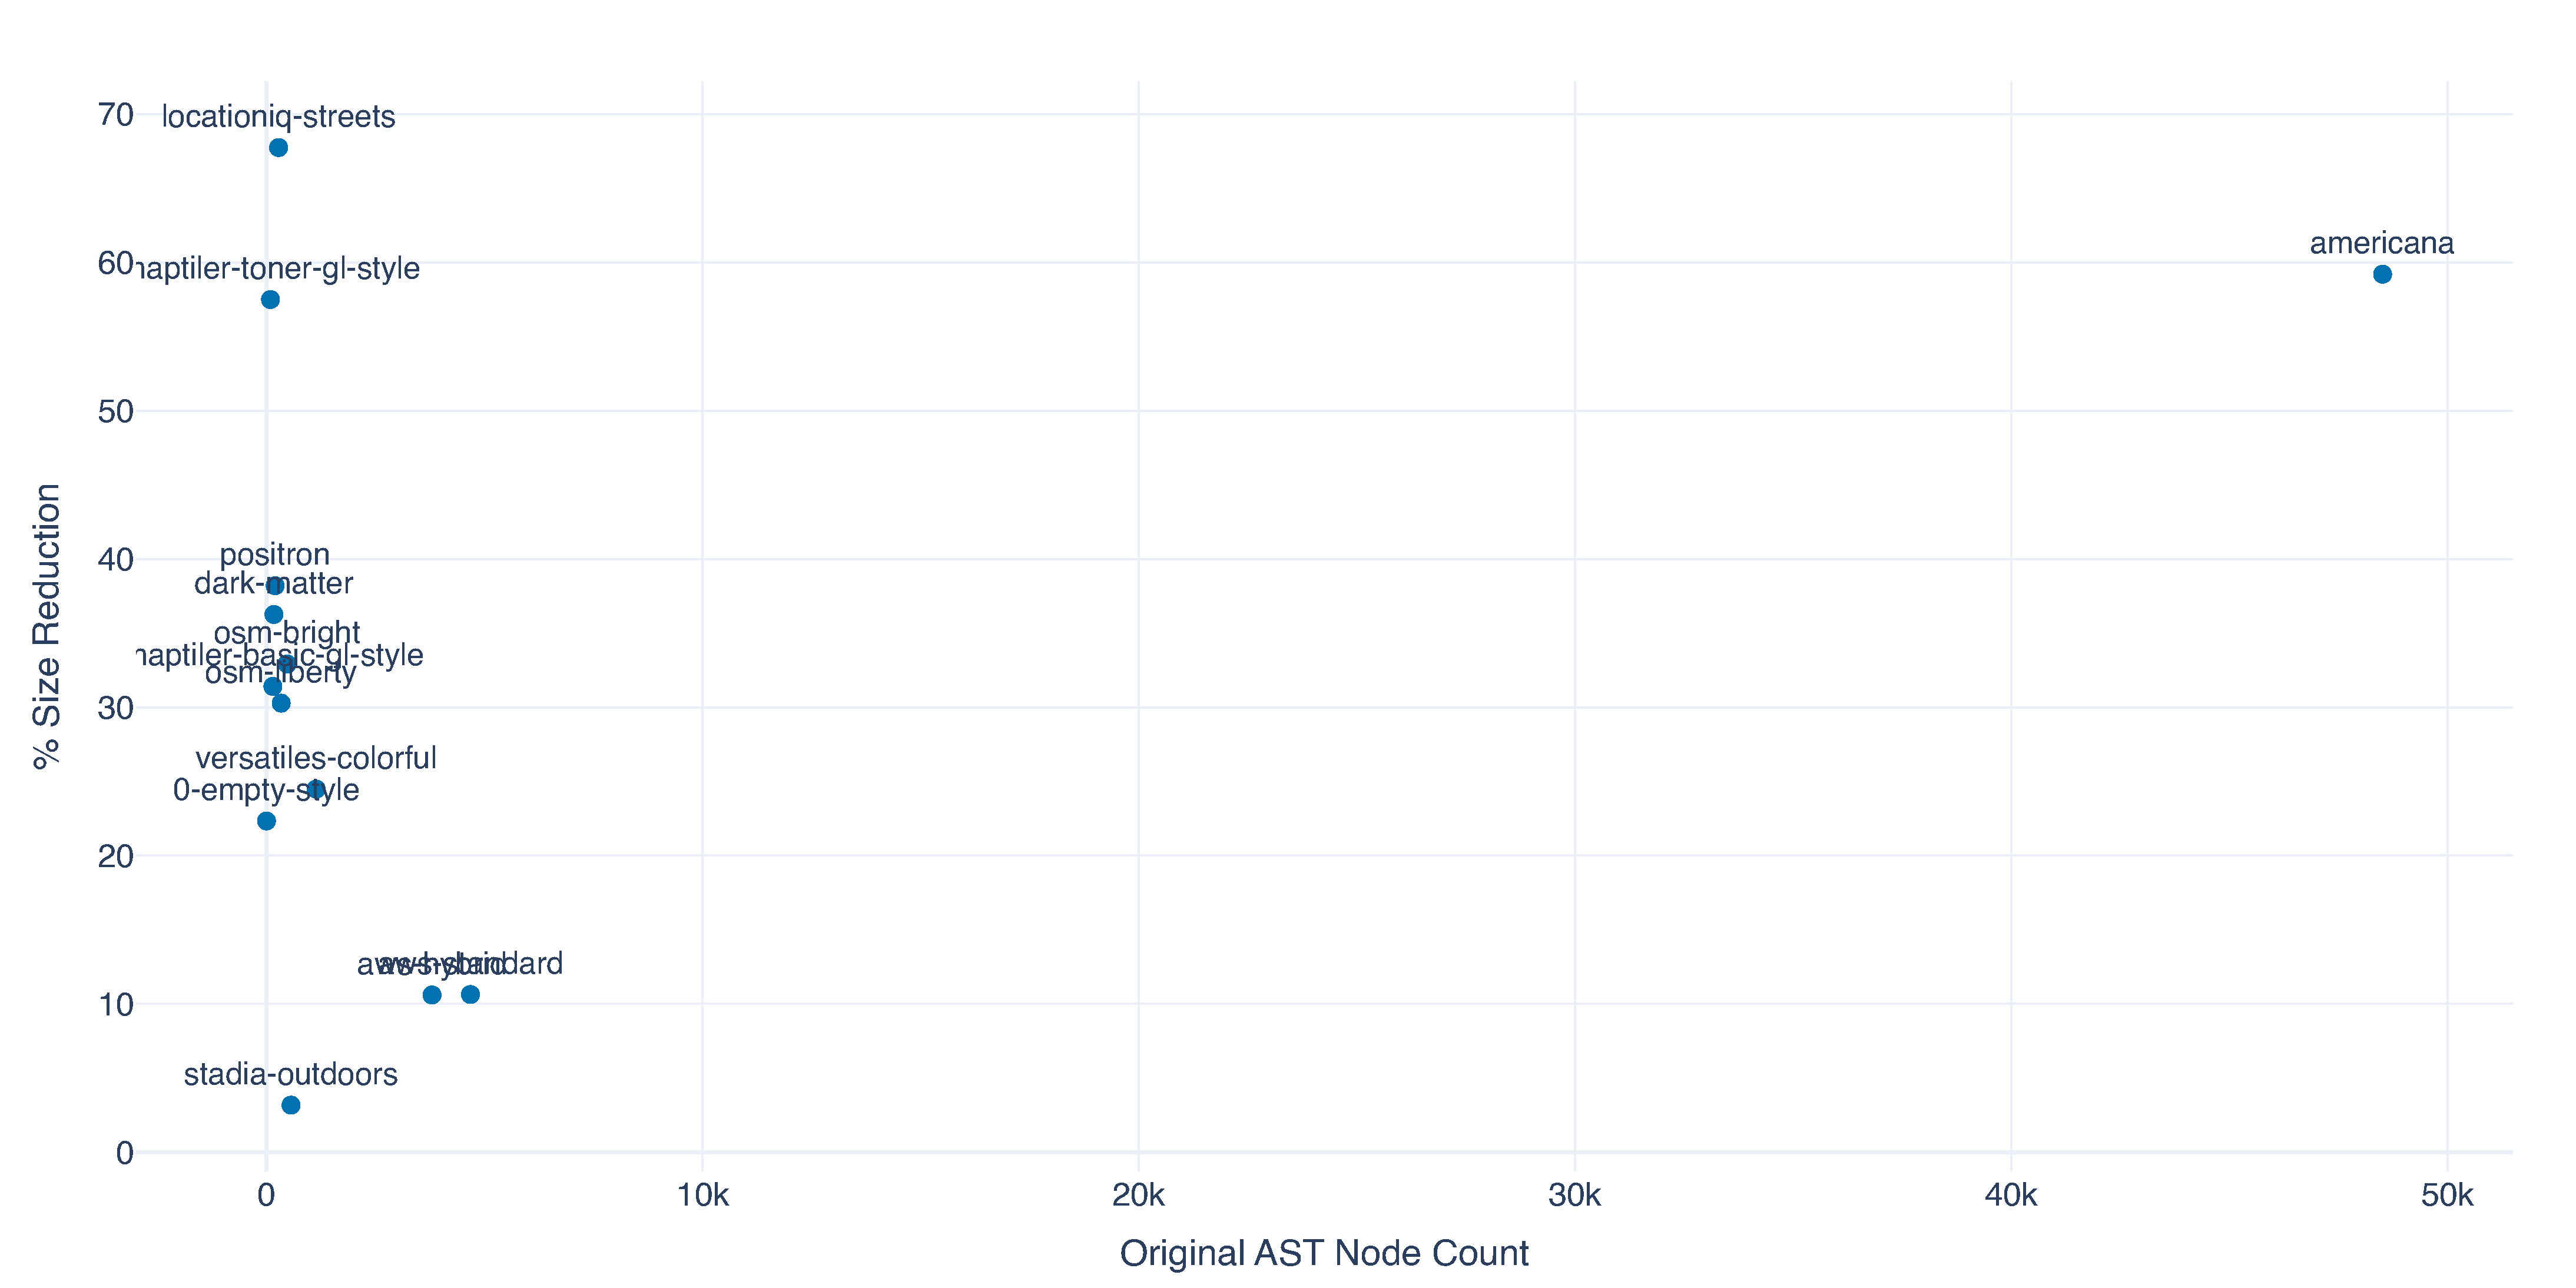
\includegraphics[width=\linewidth]{figures/cross_style_complexity_scatter.pdf}
    \caption{
Relationship between initial style complexity (\ac{AST} node count) and achievable raw style size reduction across the Maputnik generalization corpus.
The correlation is not statistically significant ($r = 0.35$, $n = 13$, $p = 0.24$), and is driven by a single high-leverage point (Americana).
Dropping it flips the sign to $r = -0.54$.
Optimization yield is therefore not reliably predictable from complexity alone, but a combination of other factors such as the cartographers' skill.}
    \label{fig:cross_style_complexity_scatter}
\end{figure}

\begin{table}[htbp]
\centering
\small
\begin{tabular}{l r r r r r}
\toprule
\textbf{Metric} & \textbf{Min} & \textbf{P25} & \textbf{Median} & \textbf{P75} & \textbf{Max} \\
\midrule
Raw size reduction (\%)         &    3.2 &   22.3 &  31.4 & 38.2 & 67.7 \\
Gzip size reduction (\%)        &    3.9 &    6.0 &  11.4 & 12.2 & 22.4 \\
Brotli size reduction (\%)      &    0.7 &    3.1 &   9.8 & 11.9 & 17.0 \\
Layer count reduction (\%)      &    0.0 &    0.8 &   4.8 &  7.0 & 27.0 \\
\ac{AST} node count change (\%) & $-269.2$ & $-102.9$ & $-47.9$ & 0.0 & 62.2 \\
\bottomrule
\end{tabular}
\caption{
Distribution of style-size and complexity changes across the Maputnik generalization corpus (13 styles, static passes only).
Median raw reduction is \qty{31.4}{\percent} and median Brotli reduction is \qty{9.8}{\percent}.
The \ac{AST}-node row is signed: positive values denote a reduction in node count, negative values denote growth from expression rewriting (e.g.\ unrolling \texttt{match} into nested \texttt{case}).
Only three of the 13 styles see a net node-count reduction, indicating that the byte-size gains come predominantly from style-level passes (default stripping, layer merging, metadata stripping) rather than from expression simplification alone.}
\label{tab:cross_style_summary}
\end{table}

\subsection{Discussion}\label{sub:cross_discussion}

The static passes deliver a median raw reduction of \qty{31.4}{\percent} (range \qtyrange{3.2}{67.7}{\percent}) across the 13 unseen Maputnik styles, with no style regressing and only a weak link between initial complexity and achievable reduction ($r = 0.35$, $p = 0.24$).
We discuss which pass families generalize universally, why we read these numbers as a lower bound on the full potential, and what the low-reduction edge cases look like in practice.

\paragraph{Universality of Expression Passes}
Expression-level passes (constant folding, boolean simplification, default stripping) produce non-zero reductions for virtually every style in the corpus, regardless of its complexity or tile schema.
We expect this: any style written by a human or generated by an editor is likely to contain at least some redundant expressions, default-valued properties, or suboptimal color encodings.

\paragraph{Complexity and Reduction}
While verbose institutional styles with several hundred layers and deeply nested expressions tend to offer more room for improvement than simple styles with fewer than 50 layers, we find that the correlation between initial style complexity and achievable reduction is not statistically significant at this sample size ($r = 0.35$, $n = 13$, $p = 0.24$), and is dominated by a single high-leverage point.
The scatter plot (\cref{fig:cross_style_complexity_scatter}) visualizes the per-style relationship.

\paragraph{Unevaluated Stats-Dependent Passes}
Because the generalization corpus does not include tile data, we cannot apply stats-driven passes (dead elimination with geometry-type matching, stats-driven constant folding, selectivity reordering) and data-level optimizations (tile shaving, re-encoding) to the Maputnik styles.
We therefore present the reported reductions as a \emph{lower bound} on the full optimizations potential.
Extrapolating from the deep corpus, where stats-driven passes add \qtyrange{10}{20}{\percent} additional reduction on top of static passes, the true optimizations potential for these styles is likely higher.
For the 11 \ac{OMT}-compatible styles in the deep corpus, we evaluated tile shaving separately against the Germany tileset (\cref{fig:tile_shave_per_style}), confirming that data-level reductions generalize across styles.

\paragraph{Edge Cases}
A small number of styles in the corpus show small reductions ($< 5\%$), the lowest being Stadia Outdoors at \qty{3.2}{\percent}.
These are typically minimal styles that already use only literal values (no expressions), have few layers, and do not set properties to their default values.
We observe no style in the corpus that shows a size \emph{increase} after optimizations, confirming that the passes are safe in the general case.
In practice, styles maintained by large organizations (which tend to accumulate verbose filters, redundant default values, and deeply nested expressions over successive authoring iterations) offer the most room for automatic simplification.
Compact basemaps authored by experienced cartographers, which already use efficient expressions and few layers, show correspondingly smaller gains.


\section{Combined Results}\label{sec:exp_combined}
\begin{keytakeaways}
\item The three optimization channels compose additively, not synergistically.
\item Data-level passes do almost nothing for sustained frame rate.
Their lever is load time.
\item No single pass dominates across styles.
The multi-pass design is what generalizes.
\end{keytakeaways}

\noindent This section presents the full pipeline ablation across all 19 cumulative steps (\cref{sub:ablation}) and analyses interactions between expression, structural, and data passes.
The combined view matters because the three categories \emph{can} interact in principle.
Style-level dead elimination narrows tile pruning advisories, and metadata refinement enables more aggressive zoom-stop pruning downstream.

\subsection{Full Pipeline Ablation}\label{sub:combined_ablation}

\cref{fig:heatmap_loadMs} presents the full scenario$\times$step load-time heatmap.
Load-time improvements are unevenly distributed across scenarios: urban, tile-dense scenarios (New York, Tokyo, Paris) show larger absolute improvements than sparse scenarios (Sahara, Amazon), because the tile-fetch component of load time dominates in dense areas.
Expression passes (steps~1-7) produce a diffuse, moderate improvement across most scenarios, whereas the improvement from structural passes (steps~8-15) is concentrated in the few styles and scenarios where dead elimination or layer merging applies.
\cref{fig:heatmap_fps} shows the companion \ac{FPS} view: the gain is broadly aligned with the load-time pattern but lands more uniformly across scenarios, because once tiles are decoded the sustained frame rate is driven by per-feature evaluation cost rather than by tile-fetch latency.

The frame-time consistency metric in \cref{fig:heatmapjankcount} worsens across the ablation as sustained frame rates push past 2000\,\ac{FPS}, where small \ac{GC}-pauses register as proportionally large outliers.
On real consumer hardware capped well below that rate the same pauses would not cross the jank threshold (see caption).

\begin{figure}[htbp]
	\centering
	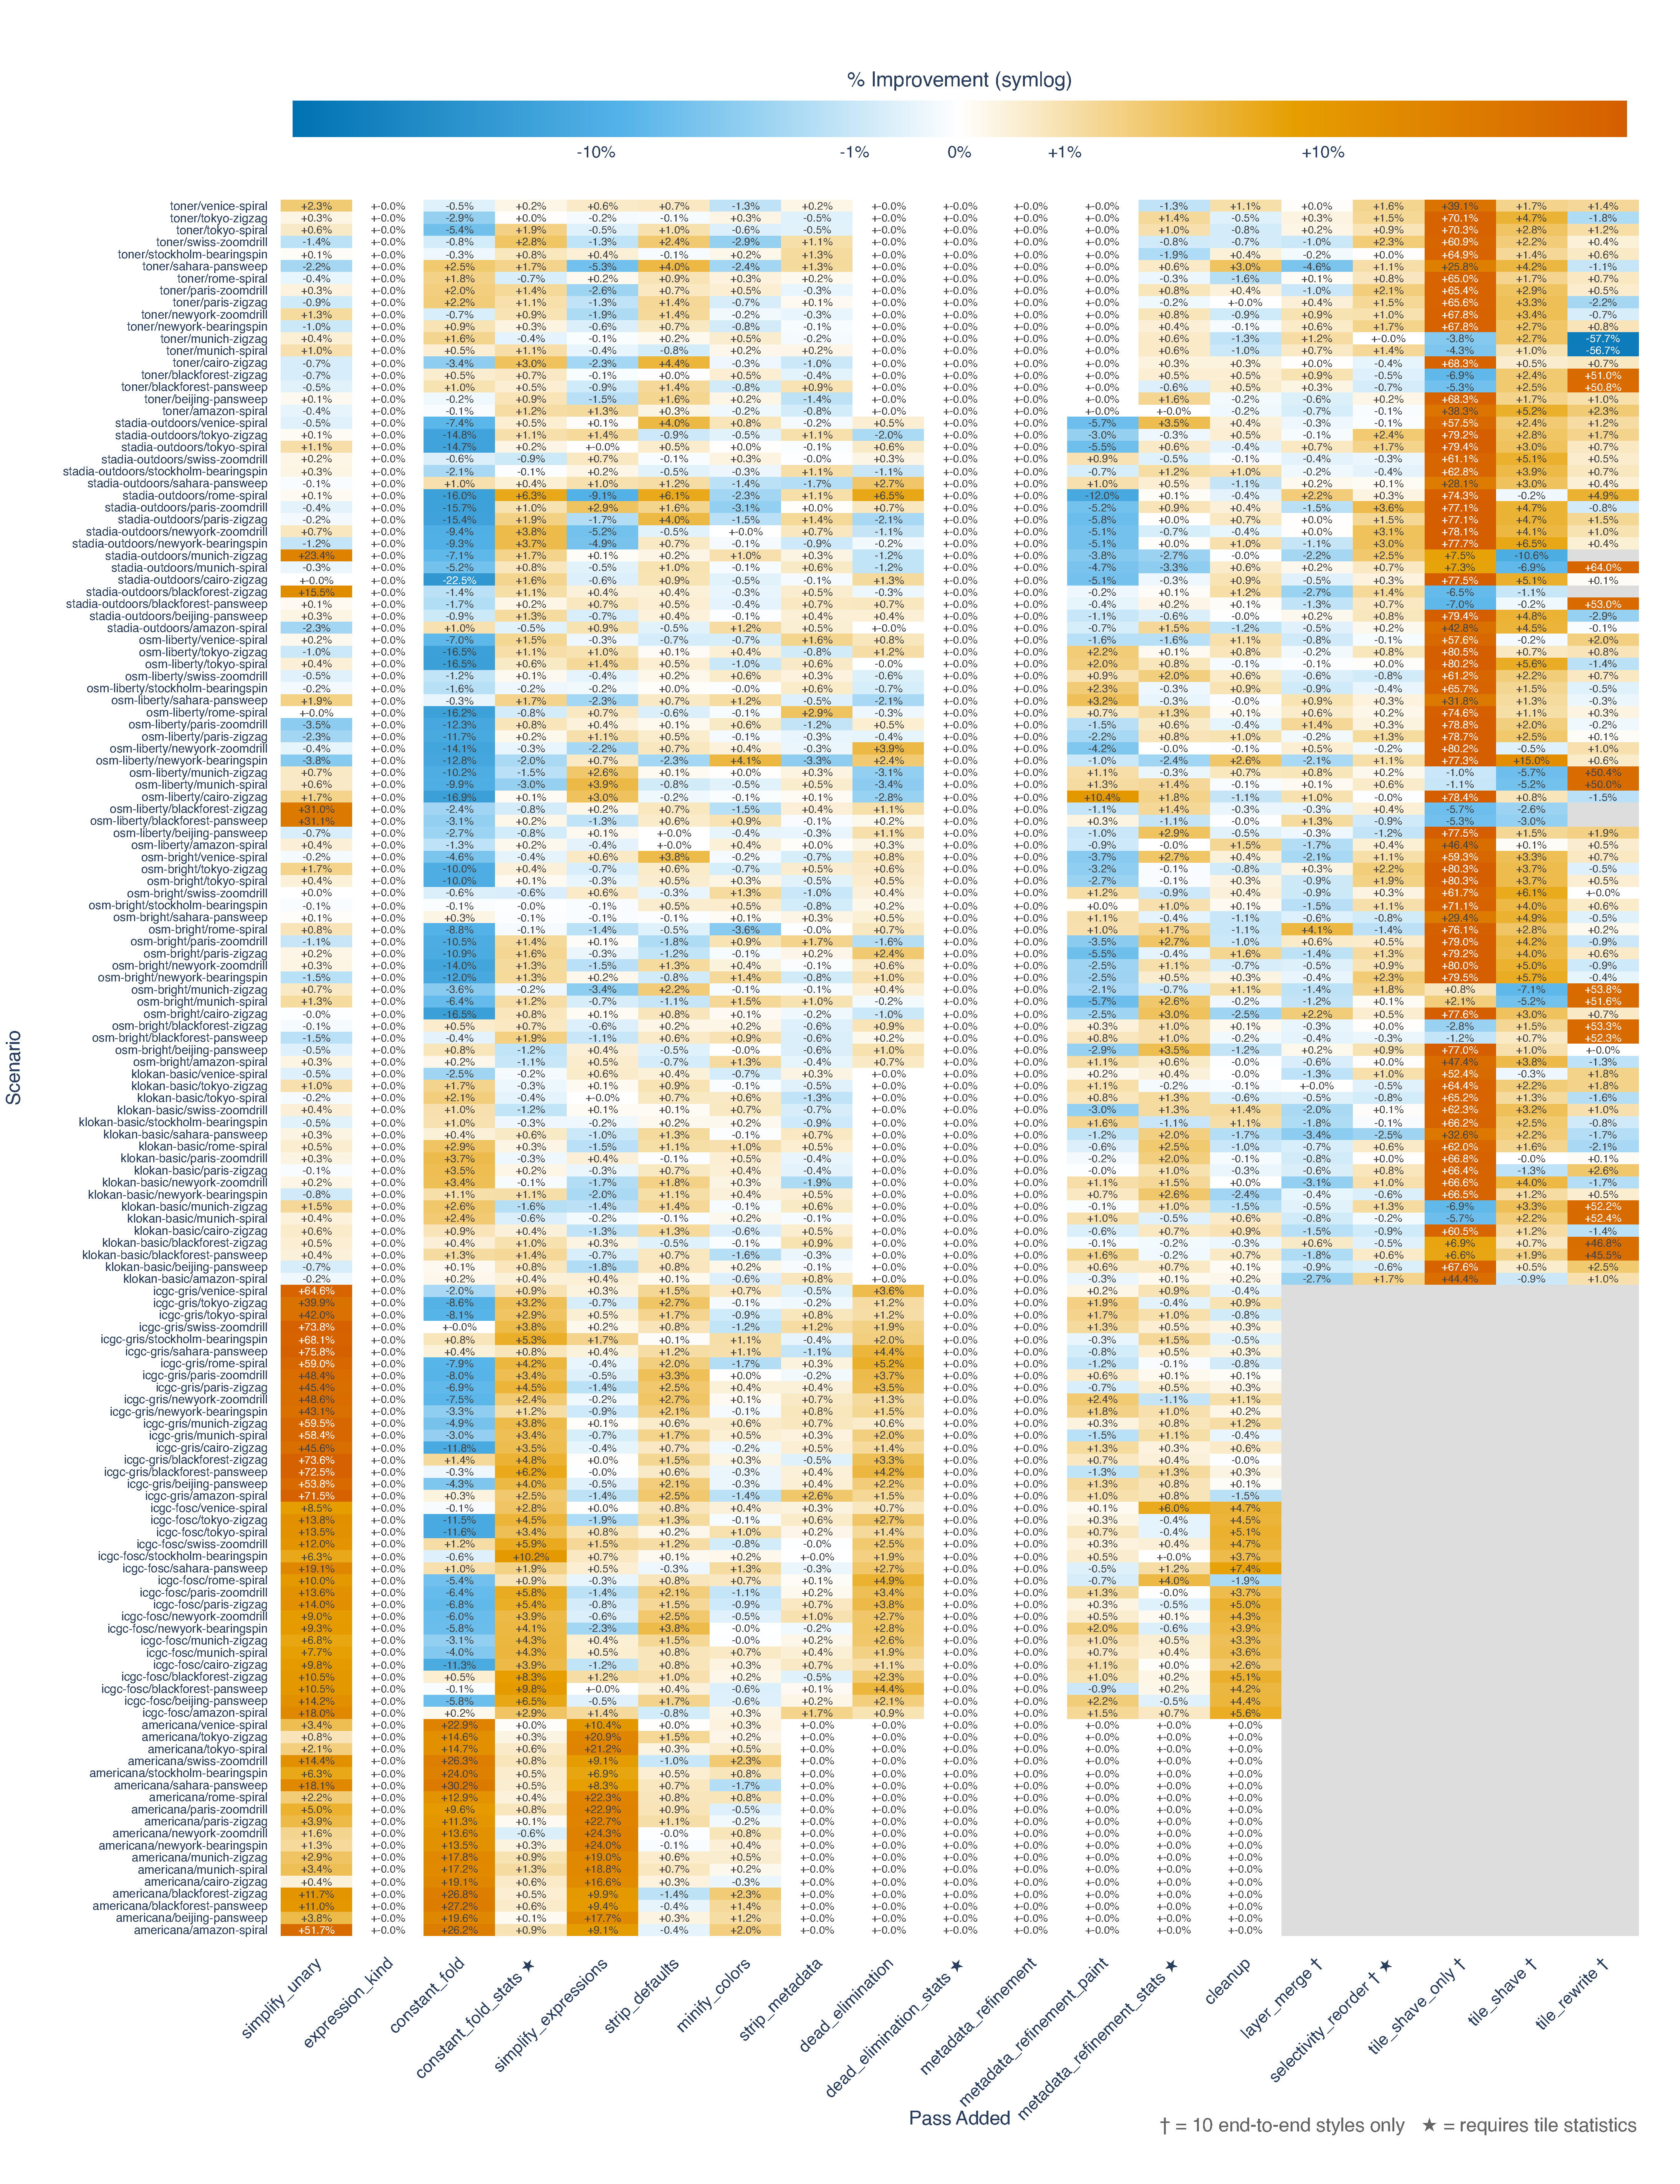
\includegraphics[height=0.9\textheight]{figures/heatmap_loadMs.pdf}
	\caption{
Heatmap of load time across scenarios (rows) and ablation steps (columns), where darker cells indicate greater improvement relative to baseline.
Urban, tile-dense scenarios (New York, Tokyo, Paris) show the largest absolute improvements.
Structural passes produce concentrated gains where dead elimination or layer merging applies.}
	\label{fig:heatmap_loadMs}
\end{figure}

\begin{figure}[htbp]
	\centering
	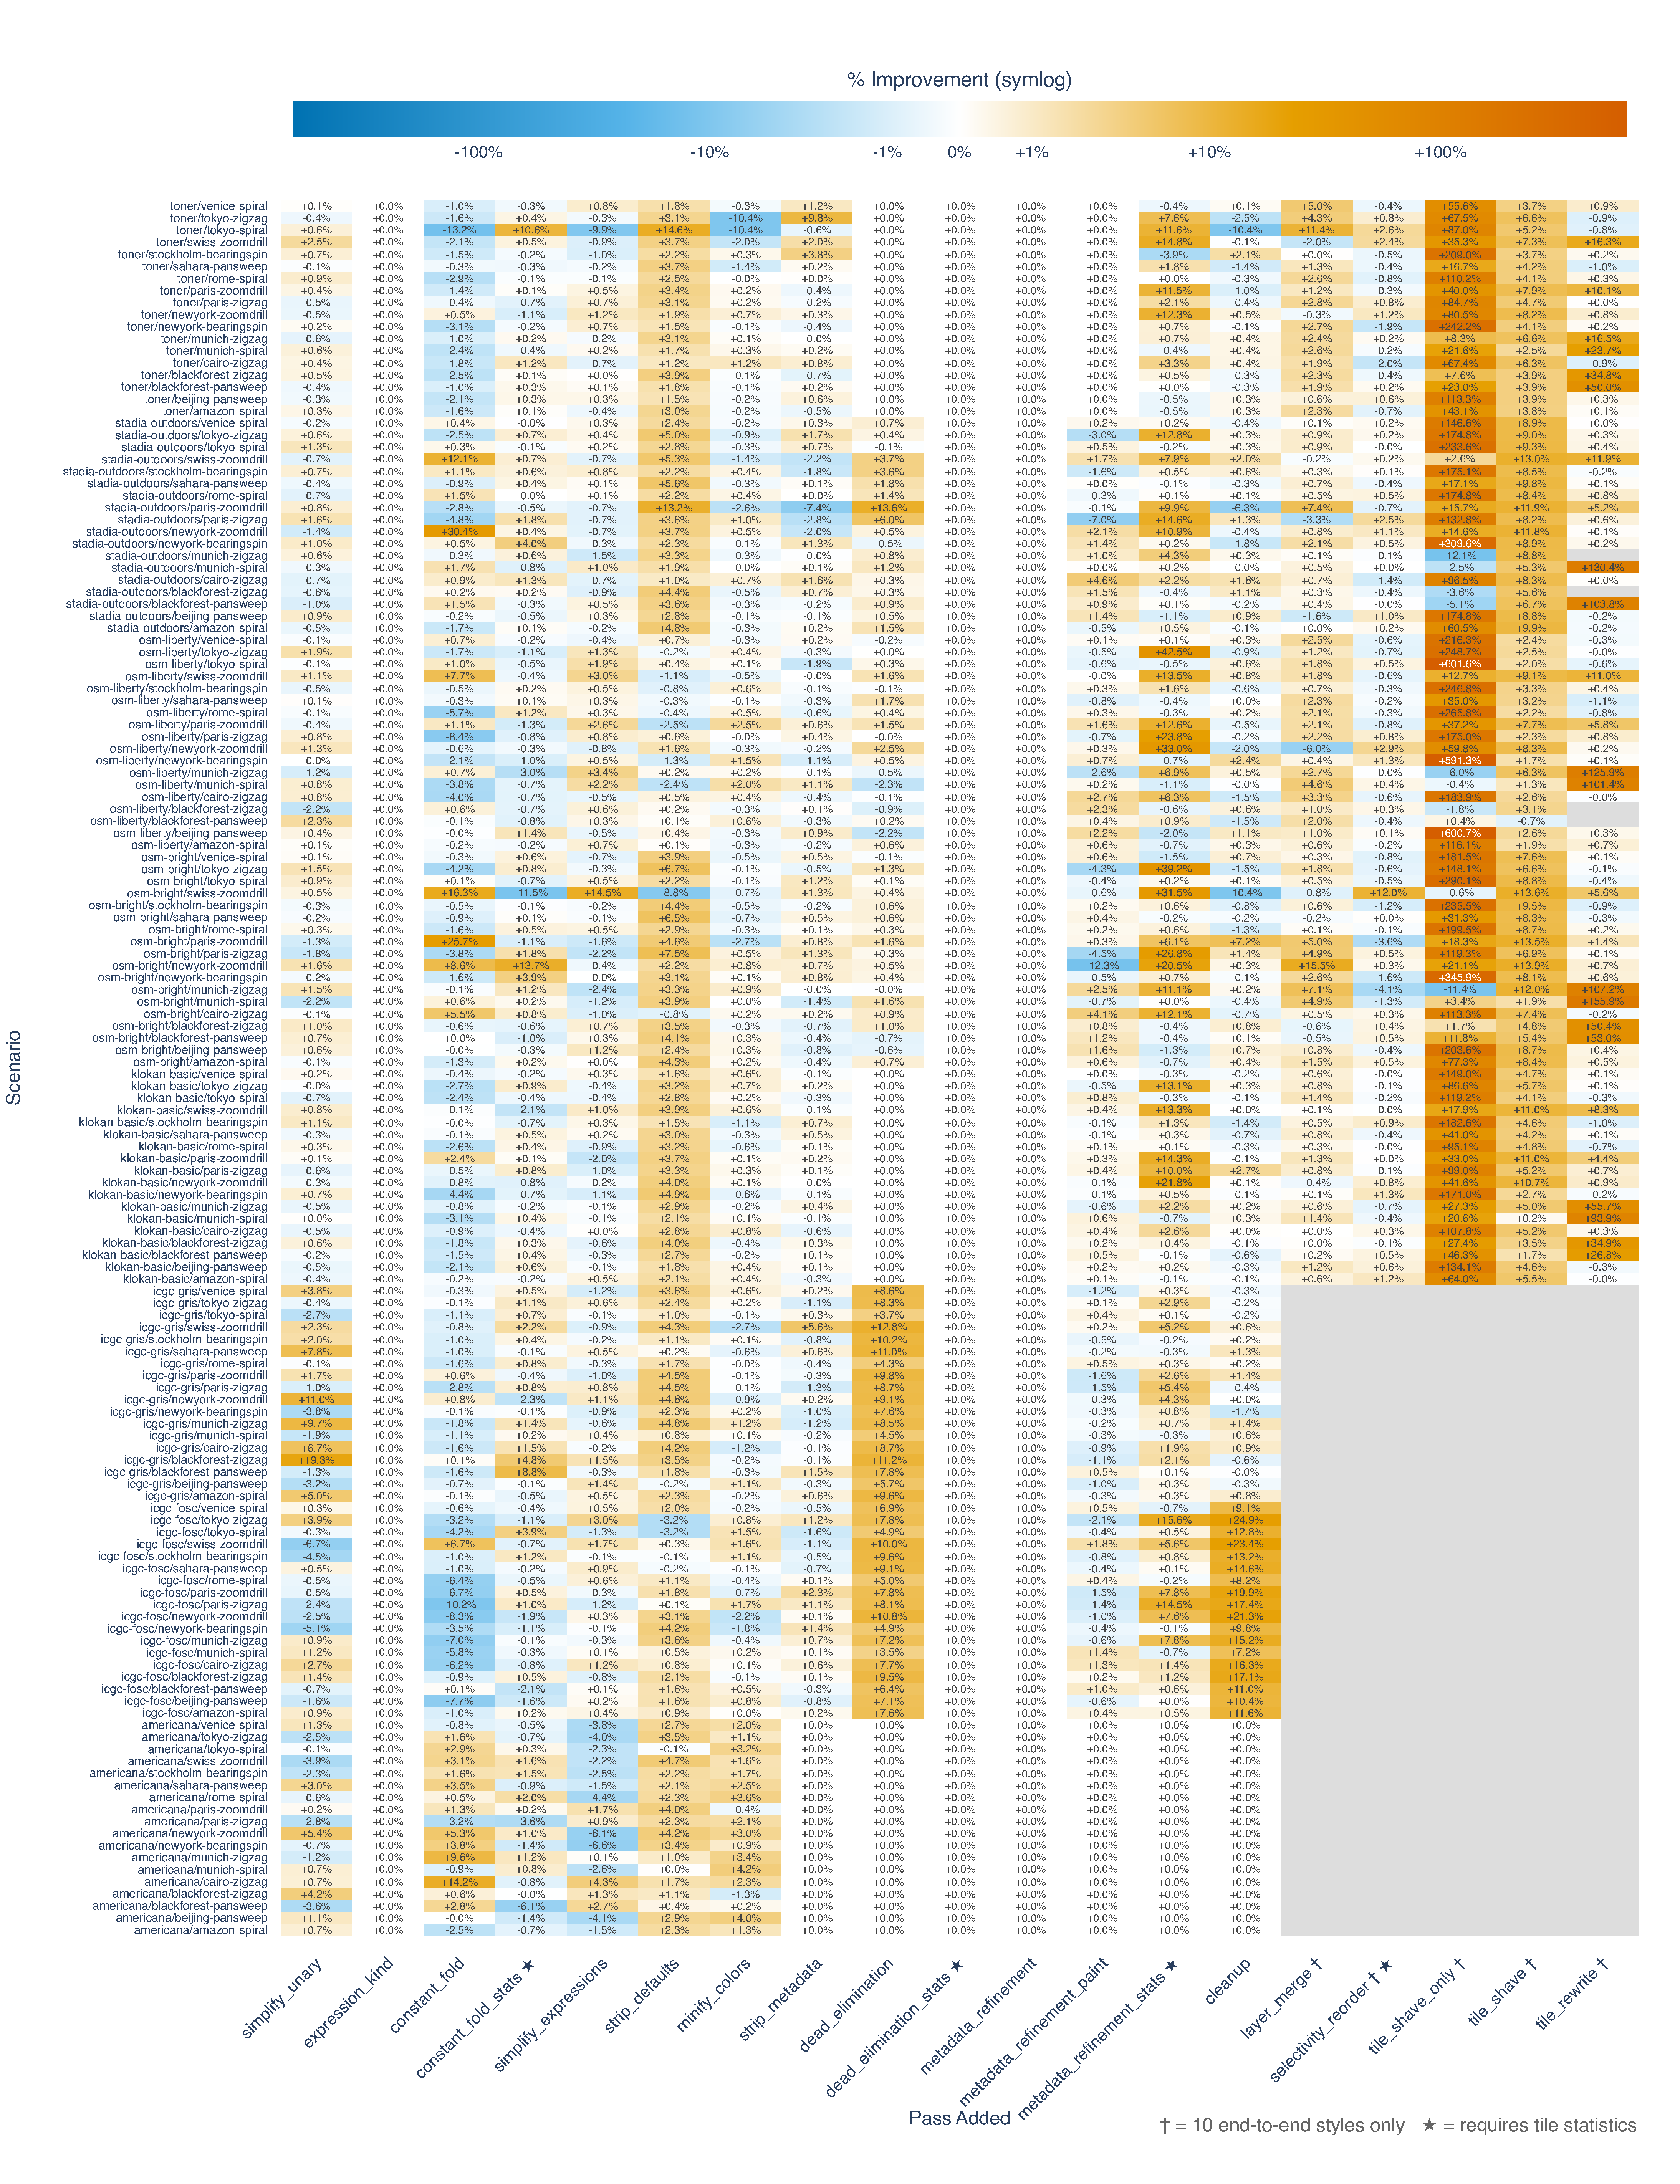
\includegraphics[height=0.9\textheight]{figures/heatmap_fps.pdf}
	\caption{
Heatmap of \ac{FPS} across scenarios (rows) and ablation steps (columns).
Compared to \cref{fig:heatmap_loadMs}, the \ac{FPS} gains are distributed more uniformly across scenarios, since sustained frame rate is driven by per-feature evaluation cost rather than by tile-fetch latency once tiles are resident.}
	\label{fig:heatmap_fps}
\end{figure}

\begin{figure}[tbph]
	\centering
	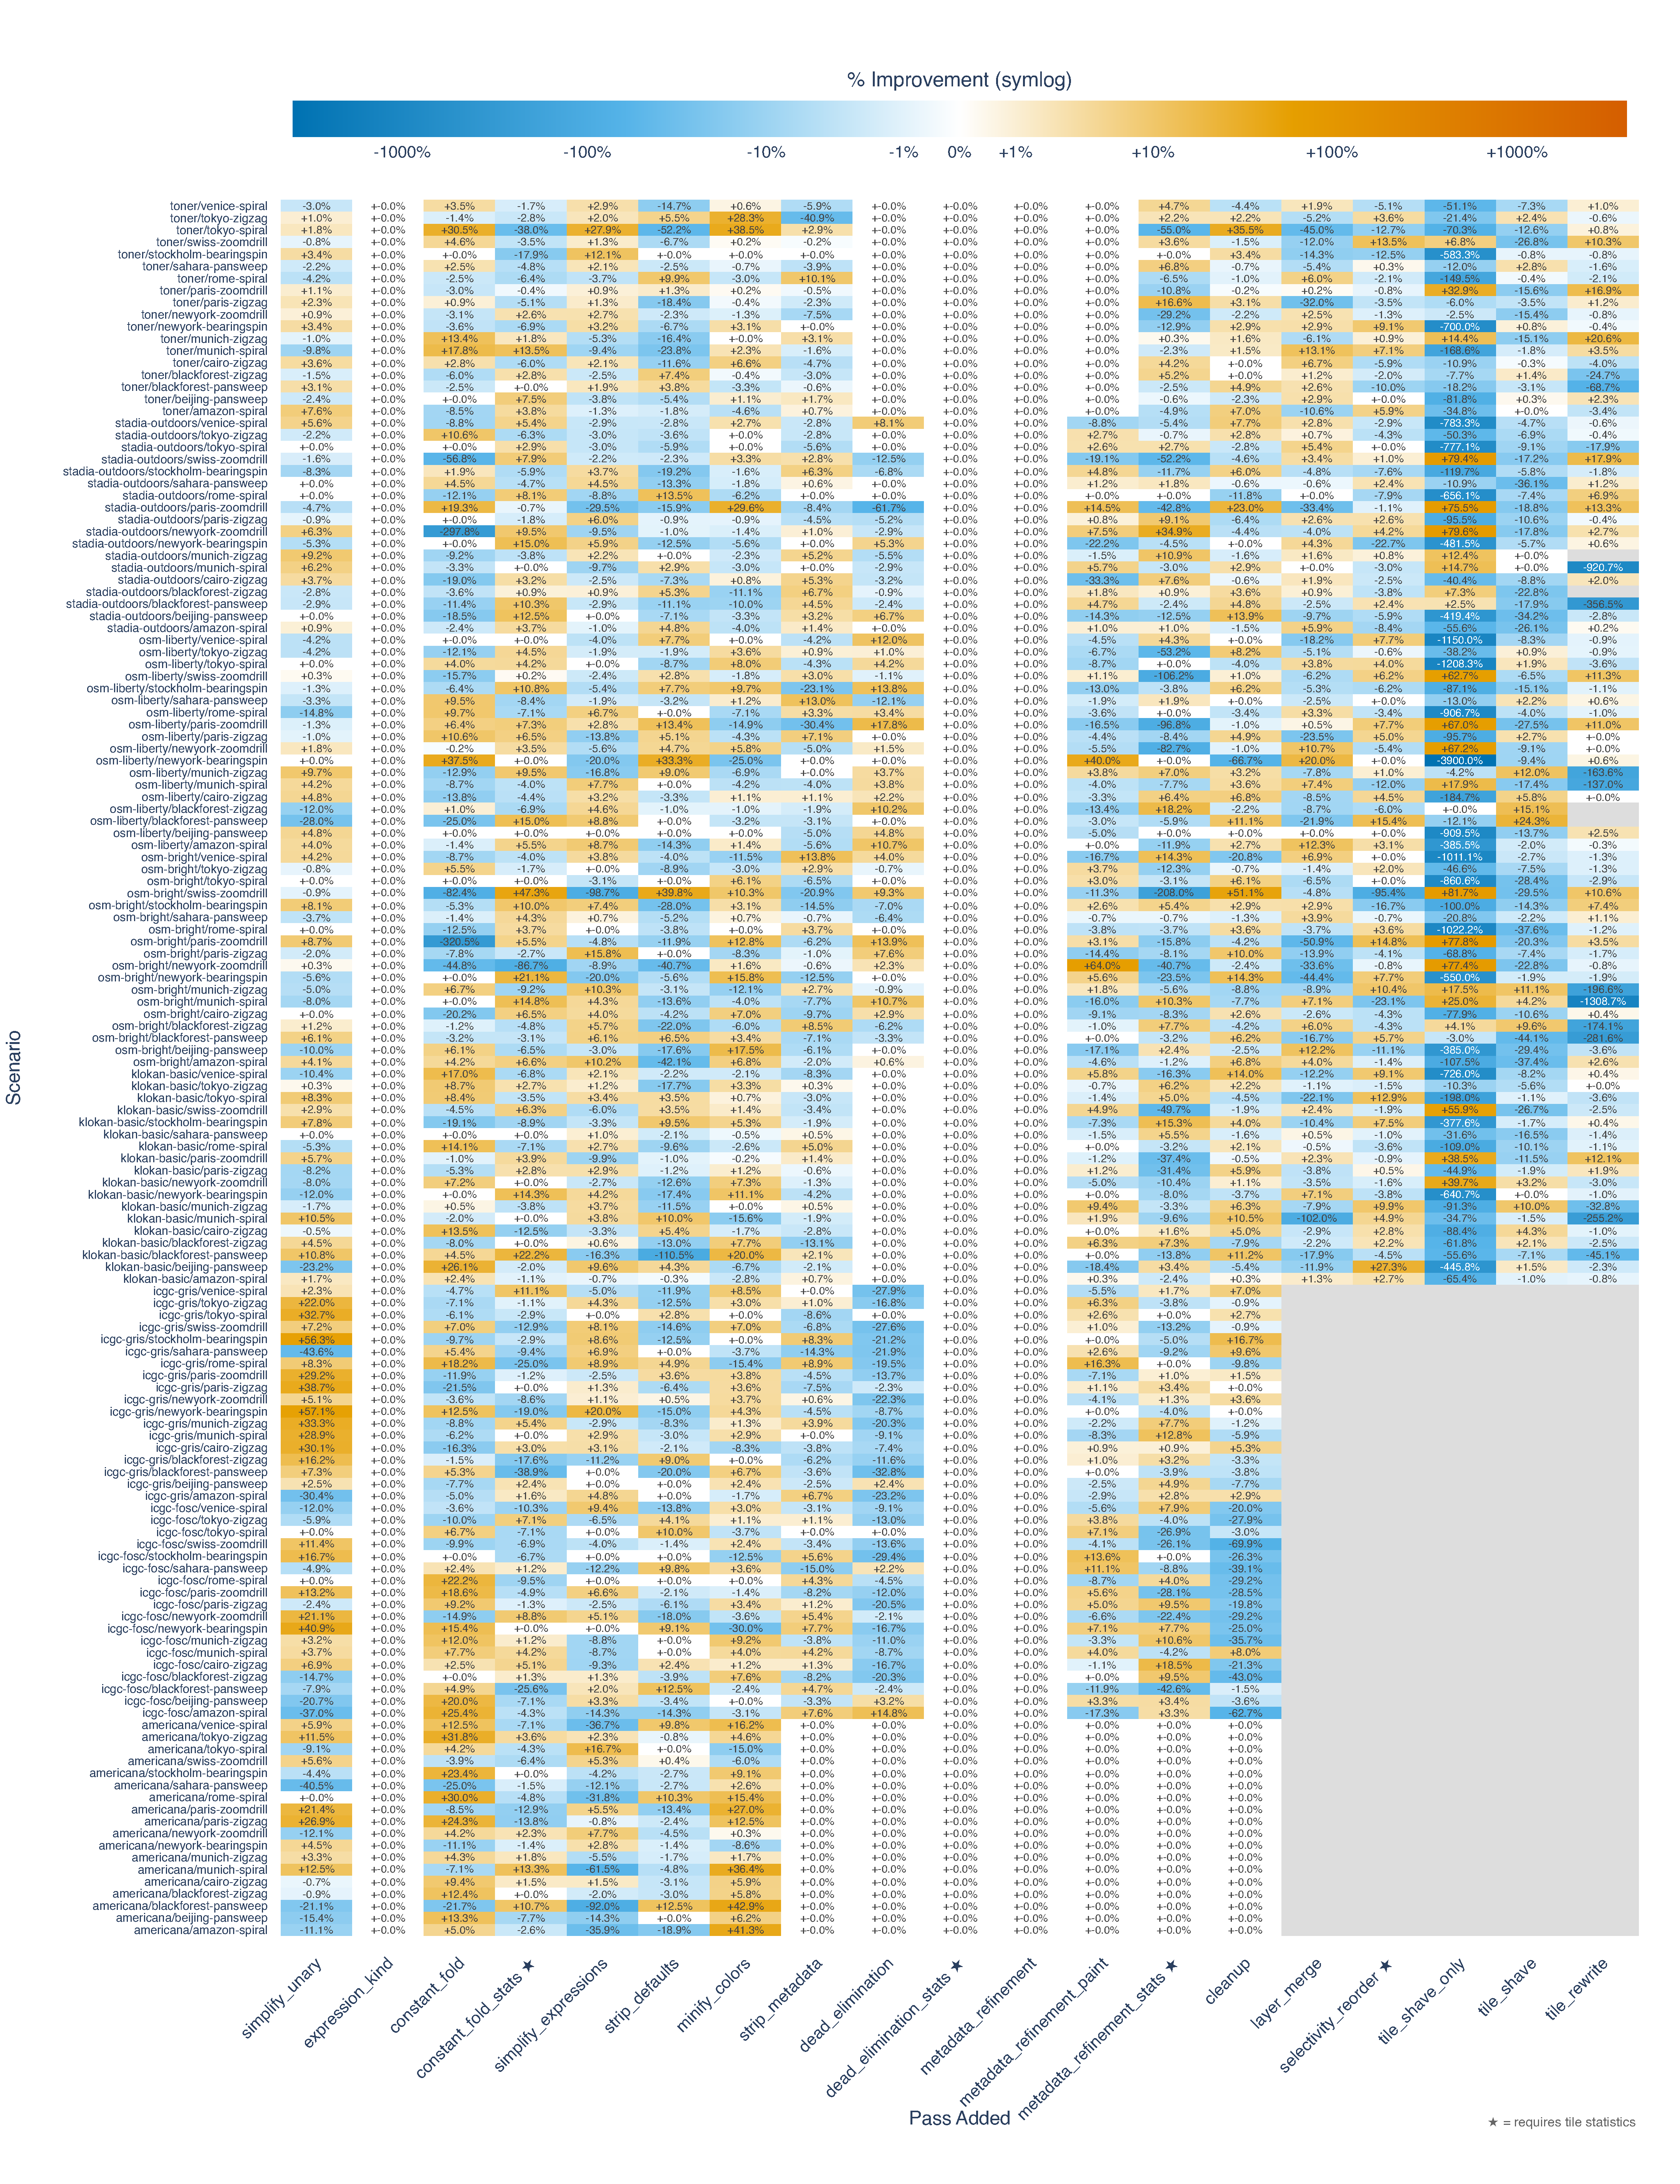
\includegraphics[height=0.9\textheight]{figures/heatmap_jankCount}
	\caption{
Heatmap of jank-frame counts (frame times substantially slower than their neighbours) across scenarios and ablation steps.
Counts increase across the ablation because sustained frame rates above 2000\,\ac{FPS} expose small \ac{GC}-pauses as proportionally large outliers.
Real consumer hardware caps well below this rate, so the same pauses would not cross the jank threshold there.}
	\label{fig:heatmapjankcount}
\end{figure}

\cref{fig:time_breakdown} decomposes load time across ablation steps.
The style-parse component shrinks monotonically with each expression pass, while first-tile and remaining-load are unchanged by style-only steps and drop only once tile shaving fires at steps~17-19.

\cref{fig:memory_ablation} tracks browser heap memory.
Style-level passes drift the resident JS heap from a baseline of \qty{86.0}{\mega\byte} to \qty{82.9}{\mega\byte} by step~15 (\qty{-3.6}{\percent}), with no single pass dominating.
Data-level passes drive the bulk of the reduction: tile shaving (step~17) alone drops the heap to \qty{63.7}{\mega\byte}, and the full pipeline reaches \qty{55.3}{\mega\byte} at step~19 (\qty{-35.7}{\percent} cumulative), reflecting that the major heap consumer is the in-memory tile payload rather than the parsed style.

\begin{figure}[htbp]
    \centering
    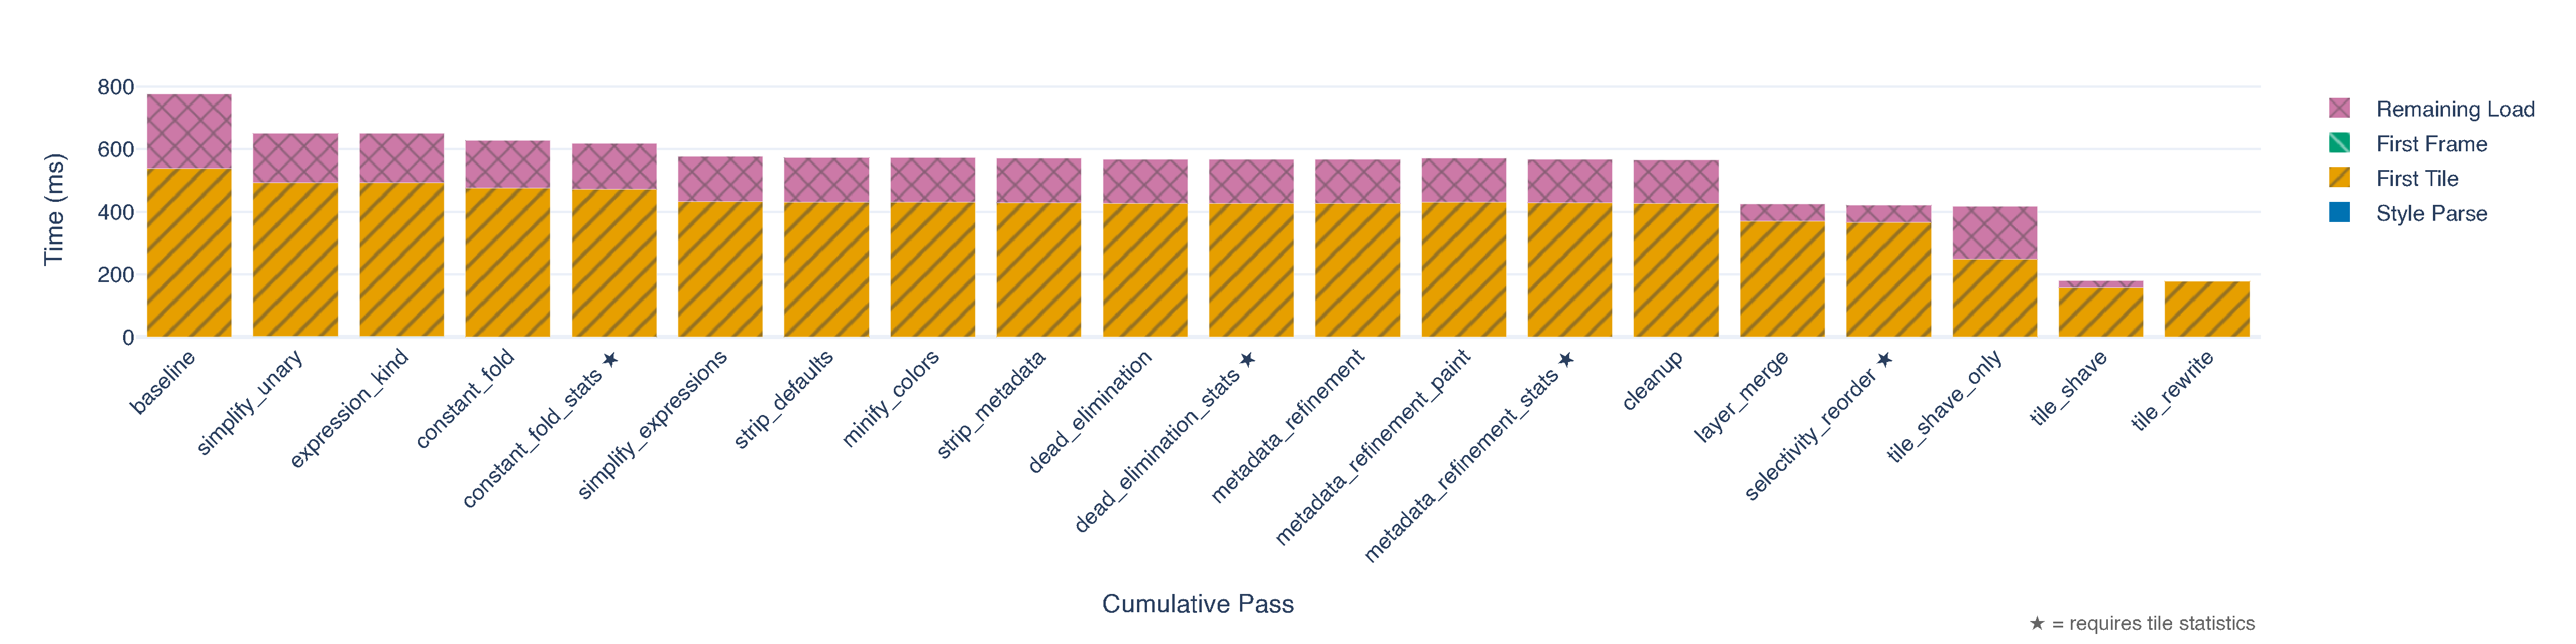
\includegraphics[width=\linewidth]{figures/time_breakdown.pdf}
    \caption{
Time breakdown across ablation steps: style parse, first tile, first frame, and remaining load time.
Style-parse time shrinks monotonically with each expression pass.
First-tile and remaining-load times are unchanged by style-only steps and decrease only when tile shaving is applied (steps~17-19).}
    \label{fig:time_breakdown}
\end{figure}

\begin{figure}[htbp]
    \centering
    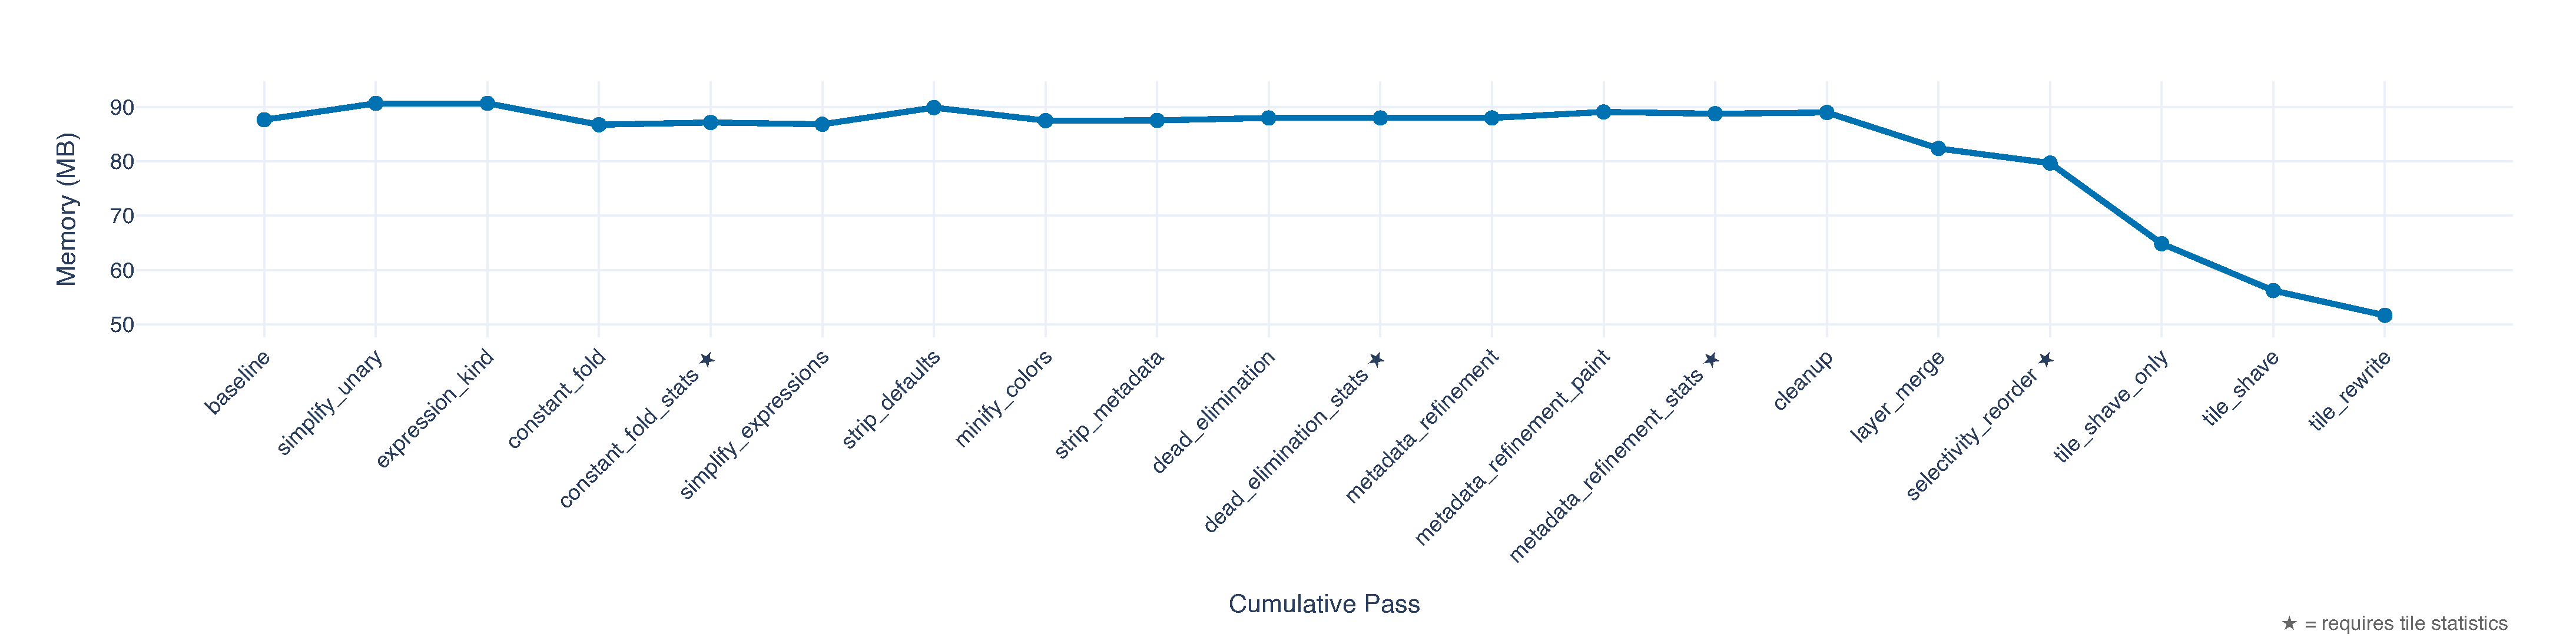
\includegraphics[width=\linewidth]{figures/memory_ablation.pdf}
    \caption{
Heap memory usage (mean \texttt{heapUsedMB} across all scenarios and benchmark styles) across ablation steps.
Style-level passes (steps 1-15) reduce the heap by \qty{3.1}{\mega\byte} (\qty{-3.6}{\percent}).
The bulk of the heap savings comes from data-level passes (steps 17-19) where the in-memory tile payload itself shrinks, yielding a cumulative reduction of \qty{-35.7}{\percent} from baseline to step~19.}
    \label{fig:memory_ablation}
\end{figure}

\begin{table}[htbp]
\centering\small
\csvreader[
  tabular=l r r r r r,
  table head={\toprule
    \textbf{Style} & \textbf{Baseline} & \textbf{Optimised} &
    \textbf{Reduction} & \textbf{$\Delta$ Load} & \textbf{$\Delta$ FPS} \\
     & \textbf{gzip (B)} & \textbf{gzip (B)} &
     \textbf{(\%)} & \textbf{(\%)} & \textbf{(\%)} \\
    \midrule},
  table foot=\bottomrule,
  head to column names,
  before line={\ifnum\midruleBefore=1\midrule\fi},
]{scripts/data/per_style_summary.csv}{}%
{\ifnum\isBold=1\textbf{\style}\else\style\fi &
 \num{\baseGzip} & \num{\optGzip} & \reduction &
 \fmtdelta{\deltaLoad} & \fmtdelta{\deltaFps}}%
\caption{
Per-style summary: baseline and optimized style size (gzip), size reduction, and change in load time and \ac{FPS} (medians across scenarios).
Styles below the rule include tile-level optimizations (steps~1-19), and those above include style-level optimizations only (steps~1-15).
Tile shaving produces the most visible drops in load time and \ac{FPS} improvements.}
\label{tab:per_style_summary}
\end{table}

\begin{table}[htbp]
\centering
\small
\csvreader[
  tabular=r l r r r r r,
  table head={\toprule
    \textbf{Step} & \textbf{Pass} & \textbf{$\Delta$ Raw} &
    \textbf{$\Delta$ Gzip} & \textbf{$\Delta$ Brotli} &
    \textbf{$\Delta$ Load} & \textbf{$\Delta$ Layers} \\
     & & \textbf{(\%)} & \textbf{(\%)} & \textbf{(\%)} & \textbf{(\%)} & \\
    \midrule},
  table foot={\midrule
    \multicolumn{7}{l}{\footnotesize $\dagger$ Steps~16-19:
    fiord and liberty only (benchmarked with tile statistics).} \\
    \bottomrule},
  head to column names,
]{scripts/data/marginal_contribution.csv}{}%
{\step & \pass\ifnum\dagger=1\textsuperscript{$\dagger$}\fi &
 \fmtdelta{\deltaRaw} & \fmtdelta{\deltaGzip} & \fmtdelta{\deltaBrotli} &
 \fmtdelta{\deltaLoad} & \fmtdeltaint{\deltaLayers}}%
\caption{
Marginal contribution of each ablation step to style size (raw, gzip, Brotli), load time, and layer count.
Values are percentage of baseline, medians across 12 styles and 18 scenarios.
Data-level tile shaving dominates transfer-size and load-time metrics.
Style-level passes contribute primarily to parse-time and style-size reductions and serve as enablers for the data-level pipeline.}
\label{tab:marginal_contribution}
\end{table}

\subsection{Marginal Contribution Analysis}\label{sub:combined_marginal}

Not all passes contribute equally, and the marginal contribution of each pass depends on the metric under consideration.

\paragraph{Rendering Time Metrics}
After tile shaving, we observe that expression-level constant folding and structural dead elimination tend to produce the largest marginal improvements in frame time and \ac{FPS}, as they reduce the number of expressions the renderer must evaluate per feature per frame and the number of layers it must process, respectively.
Layer merging produces a large marginal improvement in draw-call-heavy styles (many road layers, many boundary layers) but a smaller improvement in simple styles.

\paragraph{Transfer Size Metrics}
Passes that primarily reduce serialized style size (default stripping, metadata stripping, color minification) show smaller rendering improvements but contribute meaningfully to transfer size, particularly under compression (gzip, Brotli).
A smaller style reduces the time to first render because the \ac{JSON} must be fetched, decompressed, and parsed before the renderer can initialise.
Data-level tile shaving dominates the transfer-size metric, as tiles are fetched continuously during map interaction whereas the style is loaded only once.

\paragraph{Load Time Metrics}
Both style size (initial fetch and parse) and tile size (first tile fetch) influence load time.
Style-level passes improve style parse time.
Data-level passes improve first-tile time.
The relative contribution depends on the network bandwidth.
Under the \qty{10}{\Mbps} throttle, tile-fetch latency dominates.
Under the \qty{1.5}{\Mbps} throttle, style-fetch latency becomes significant for large styles.

\subsection{Preprocessing Cost}\label{sub:preprocessing_cost}

Research Goal~R3 asks how expensive the optimizations are in terms of preprocessing time.
The optimizations pipeline is an \emph{offline} stage: we optimize a style once and serve it many times, and re-encode tiles once per tileset build.
Preprocessing cost is therefore amortised over all subsequent tile deliveries and is not on the user's critical path, but it still matters for operational feasibility on large tilesets.

In this section we measure each of the four additive cost terms $C_\text{style}$, $C_\text{stats}$, $C_\text{adv}$, and $C_\text{enc}$ from the preprocessing cost model (\cref{eq:cost_model}, \cref{sub:preprocessing_cost_model}) on a real tileset, and confirm that the cost-control mechanisms formalised there keep the multi-strategy overhead well below the naive worst case.

\paragraph{Measured Stage Costs}
\Cref{tab:preprocessing_cost} reports wall-clock time for each stage of the preprocessing pipeline on the Germany OpenMapTiles tileset (\num{256156} tiles after pruning, zoom 0-14), which we measured on an AMD Ryzen~7 3700X (8 cores / 16 threads), \qty{46}{\gibi\byte} \ac{RAM}, NVMe SSD (median of three runs).
\emph{Style optimization} ($C_\text{style}$) and \emph{advisory computation} ($C_\text{adv}$) are negligible: Liberty's 111-layer style completes all passes in \qty{7.5}{\milli\second} and the advisory in \qty{1.1}{\milli\second}.
\emph{Tile-statistics collection} ($C_\text{stats}$) takes \qty{57.4}{\second} for a single-threaded scan of all \num{256588} source tiles.
\emph{Tile pruning and \ac{MVT} re-encoding} ($C_\text{enc}$, MVT) takes \qty{15.6}{\second} using Rayon\footnote{\url{https://github.com/rayon-rs/rayon}, last accessed 2026-05-23} parallelism.
\emph{\ac{MLT} encoding with sort-strategy competition} ($C_\text{enc}$, \ac{MLT} auto) is the dominant term: \qty{5}{\minute}\,\qty{42}{\second} single-threaded, or \qty{47}{\second} with 16 threads.
Without the competition ($C_\text{enc}$, \ac{MLT} none), single-threaded encoding takes \qty{2}{\minute}\,\qty{55}{\second}.
We therefore measure the overhead ratio of the full competition at $342 / 175 = 1.95\times$ in \ac{CPU} time, substantially lower than the analytical 3-5$\times$ estimate, because the cost-control mechanisms formalised in \cref{sub:preprocessing_cost_model} eliminate most redundant work.

\begin{table}[htbp]
\centering\small
\begin{tabular}{l l r}
\textbf{Stage} & \textbf{Description} & \textbf{Wall-clock} \\
\midrule
$C_\text{style}$ & Style optimization (all passes, Liberty) & \qty{7.5}{\milli\second} \\
$C_\text{stats}$ & Tile statistics (\num{256588} tiles, 1 thread) & \qty{57.4}{\second} \\
$C_\text{adv}$ & Advisory computation & \qty{1.1}{\milli\second} \\
$C_\text{enc}$ (\ac{MVT} prune) & Tile pruning + \ac{MVT} re-encode (16 threads) & \qty{15.6}{\second} \\
$C_\text{enc}$ (\ac{MLT} none, 1T) & \ac{MLT} encoding, single strategy, 1 thread & \qty{175}{\second} \\
$C_\text{enc}$ (\ac{MLT} auto, 1T) & \ac{MLT} encoding, full competition, 1 thread & \qty{342}{\second} \\
$C_\text{enc}$ (\ac{MLT} auto, 16T) & \ac{MLT} encoding, full competition, 16 threads & \qty{46.7}{\second} \\
\midrule
Overhead factor & auto\,/ \,none (single-threaded CPU time) & $1.95\times$ \\
\end{tabular}
\caption{
Preprocessing wall-clock time per pipeline stage on the Germany OpenMapTiles tileset (zoom 0-14, \num{256156} tiles after pruning) when run on \cref{tab:bench_hardware}.
Median of 3~runs.
Style optimization ($C_\text{style}$, \qty{7.5}{\milli\second}) and advisory computation ($C_\text{adv}$, \qty{1.1}{\milli\second}) are negligible; \ac{MLT} encoding with full sort-strategy competition dominates at \qty{342}{\second} single-threaded (\qty{46.7}{\second} with 16 threads), with an overhead factor of $1.95\times$ vs.\ a fixed-plan encoder.}
\label{tab:preprocessing_cost}
\end{table}

\paragraph{Amortisation and Headline Numbers}
Taken together, the cost-control mechanisms formalised in \cref{sub:preprocessing_cost_model} (bounding-box pruning, data profiling, warm-start caching, scratch-buffer recycling, and the \ac{RAII} alternatives guard) reduce the measured overhead of the full sort-strategy competition to $1.95\times$ compared to a fixed-plan (single-strategy) encoder (\cref{tab:preprocessing_cost}), well below the naive $4\times$ expectation from four candidate sort orders.
We empirically confirm that the trial-and-retain loop costs $k$ encode passes plus $\mathcal{O}(1)$ bookkeeping rather than $k$ encode passes plus $k$ full buffer clones.
We pay this cost once per tileset build and amortise it over every subsequent tile request.
The total single-threaded pipeline time (statistics collection through \ac{MLT} encoding with full competition) is under \qty{7}{\minute} on the Germany tileset.
With 16-thread parallelism the end-to-end wall-clock time drops to approximately \qty{2}{\minute}, perfectly acceptable for an offline build stage.
The effect of this on client side performance is not as big as it could currently be, because internally we transform data to \acsp{MVT} instead of a more efficient in-memory-structure.

\subsection{Complexity Metrics}\label{sub:combined_complexity}

The four complexity metrics we track across ablation steps (\cref{sub:metrics}) give a structural explanation for the observed rendering improvements.
Expression passes (constant folding, simplification) drive the largest reductions in \ac{AST} node count.
Boolean flattening and De~Morgan rewrites drive the maximum-depth reductions.
Dead elimination and layer merging drive the layer-count reductions.
Metadata refinement (by consuming zoom predicates) together with dead elimination drive the filter-count reductions.
Where the same step appears across two complexity axes, we describe the connection to the corresponding rendering metric in \cref{sub:combined_marginal}.

\subsection{Discussion}\label{sub:combined_discussion}

Composed end-to-end across the ten deep-corpus styles, the full pipeline cuts per-style median load time by \qty{71}{\percent} and lifts \ac{FPS} by \qty{152}{\percent}.
The three optimization channels (expression, structural, data) compose additively because they target non-overlapping costs (simplification cannot shrink tiles, shaving cannot prune expressions).
The following paragraphs decompose which channel each family acts on, separate the load-time levers from the frame-rate levers, and close with the measurement-noise caveats that bound these numbers.

\paragraph{Three Plausible Improvement Channels}
The full pipeline ablation points to three plausible channels, which we infer from proxy metrics (\ac{AST} node count, layer count, tile size) and the time breakdown (\cref{fig:time_breakdown}) since no renderer instrumentation separates them directly.
The expression passes (\cref{sub:expression_optimizations}) plausibly reduce per-feature evaluation cost.
Fewer \ac{AST} nodes mean fewer interpreter steps per feature per frame.
Dead elimination and layer merging (\cref{sub:structural_optimizations}) operate one level up, cutting draw calls, \ac{GPU} state changes, and per-layer filter evaluations.
Tile shaving and re-encoding (\cref{sub:data_optimizations}) act on transfer and decode cost so load time and time-to-first-tile drop, with a secondary effect on average frame time via lower \ac{GC}-spend.

\paragraph{Load Time vs.\ Frame Rate}
Expression and structural passes improve both load time and frame rate, because a simpler style is both faster to parse and faster to render.
Data-level passes primarily improve load time (smaller tiles arrive faster) and have a smaller effect on sustained frame rate, since once tiles are decoded and resident in the \ac{GPU} the per-frame cost is dominated by expression evaluation and draw-call overhead rather than data size.
The exception is tile shaving at overview zoom levels, where removing entire source-layers reduces the number of features the renderer must process per frame.

\paragraph{What Varies, and Why}
The cumulative ablation shows diminishing marginal returns:
early passes (constant folding, dead elimination) capture the largest improvements because they address the most common sources of waste, while later passes (color minification, metadata stripping) address less frequent patterns and contribute correspondingly less.
The non-cumulative isolated-impact analysis confirms that each pass has a non-trivial standalone contribution, even when its cumulative-sequence contribution looks small.
The marginal number is sensitive to which passes precede it, but the standalone number is not.

Variation across styles is similarly structured:
styles with many narrowly-filtered layers (e.g.\ detailed road styles) benefit most from layer merging, styles with broad filters from stats-driven dead elimination, and styles with large expression trees from constant folding.
No single pass dominates across all styles, which is the empirical justification for the multi-pass design.

\paragraph{Measurement Noise}
The 15-run median smooths out most measurement noise, but tail metrics (p99 frame time, jank count) carry higher variance than central-tendency metrics; \ac{GPU} thermals, browser garbage collection, and OS scheduling all contribute.
We partly self-inflict this: using real \ac{GPU} hardware (ANGLE/Vulkan) rather than a software rasteriser captures realistic rendering costs (\ac{GPU} buffer management, shader compilation) at the expense of slightly higher noise compared to deterministic software rendering.


\section{Visual Correctness Validation}\label{sec:visual_correctness}

We verified visual losslessness (\cref{eq:visual_equivalence}, with the per-pass soundness arguments collected in \cref{sec:building_optimizations}) with pixelmatch\footnote{\url{https://github.com/mapbox/pixelmatch}, last accessed 2026-05-23} across all 15 benchmark styles at zoom levels~0-14, across all 18 scenarios from \cref{sub:scenarios}, in both axis-aligned and pitched views, at \texttt{pixelRatio}~1 and using MapLibre GL~JS's Node-side software rasteriser.
Across every comparison, the fraction of differing pixels stayed below pixelmatch's per-test tolerance (default \texttt{allowed}~$=0.00025$ at the YIQ-perceptual \texttt{threshold}~$=0.1285$), confirming that every optimizations pass preserves visual identity on the software rasteriser within the perceptual-difference budget used by the upstream MapLibre render harness.

\section{Threats to Validity}\label{sec:threats}

In this section we discuss potential threats to the validity of the experimental findings.

\paragraph{Internal Validity}
We conducted all rendering benchmarks on a single hardware configuration (\ac{GPU} model, \ac{CPU}, memory) running a specific browser version with ANGLE/Vulkan as the graphics backend.
The full host, driver, toolchain, and dependency dump is in \cref{app:bench_env}.
Performance characteristics may differ on other hardware or with different graphics backends (e.g., native OpenGL, DirectX, Metal).
We chose the 15-run median to reduce measurement noise, but rare performance events (e.g., \ac{GPU} thermal throttling, garbage collection pauses) may not be fully captured.
The caching proxy eliminates network variability but also prevents observation of real-world caching effects and \ac{CDN} behavior.

\paragraph{External Validity}
We limit the evaluation to MapLibre GL~JS.
Results may not transfer directly to other renderers such as Mapbox GL~JS, deck.gl, or native MapLibre implementations.
The tile data uses only OpenMapTiles and BasemapDE schemas.
Other schemas with different property distributions or geometry characteristics may yield different optimizations gains.
The 15 benchmark styles, while diverse, may not represent all style authoring patterns encountered in production deployments.

\paragraph{End-to-End Data-Level Coverage}
We benchmark the full rendering pipeline (style optimizations through tile shaving to \ac{MLT} re-encoding) end-to-end on 10 of the 15 deep-corpus styles (bright, dark-matter, fiord, klokan-basic, liberty, osm-bright, osm-liberty, positron, stadia-outdoors, toner).
ICGC Fosc and ICGC Gris were excluded because the legacy \mlprop{\texttt{text-field}} handling described in \cref{sub:deep_corpus} renders incorrectly under MapLibre's silent migration.
The BasemapDE pair was excluded because its tile source is not \ac{OMT}-compatible and we could not provision matching shaved tiles.
For the remaining \ac{OMT}-compatible deep-corpus styles we verified the tile-shaving step alone (advisory generation and \ac{MVT} pruning, without rendering) on the same Germany tileset (\cref{fig:tile_shave_per_style}), confirming that shaving effectiveness generalizes across styles with reductions of \qtyrange{19.8}{46.3}{\percent}.
The remaining limitation is that tile statistics at a sample rate of~1.0 require access to the underlying tile data, which is available only for \ac{OSM}-based tilesets accessed via a local \texttt{.mbtiles} file.
The style-only results (Experiments~1-2) cover all 15 styles and are not affected by this limitation.

\paragraph{Construct Validity}
We simulate network conditions via a fixed bandwidth throttle (\cref{sub:tile_data}) rather than measuring under real \ac{CDN} latency profiles.
We designed the synthetic camera animations of \cref{sub:scenarios} (zigzag, spiral, zoomdrill, pansweep, bearingspin) to exercise diverse rendering workloads, but they may not capture typical user interaction patterns such as search-and-zoom workflows.

\paragraph{Statistical Validity}
The tile statistics (\cref{sub:tile_statistics}) count feature \emph{occurrences} across tiles, not unique geographic entities: a highway spanning 50 tiles is counted 50 times.
This inflates total feature counts and distorts absolute selectivity estimates, though relative selectivity ordering (which is all the reordering heuristic of \cref{sec:selectivity_reordering} consumes) is less affected.
We made this choice deliberatiley because the underlying features are not a concearn for the renderer on most layers (exception being symbol placement which is map-global instead of tile-local).

The selectivity estimation model assumes independence between filter predicates (\cref{eq:selectivity_compound}), which may not hold for correlated properties.
Map-style filters in practice do exhibit correlations (e.g.\ \mlval{\texttt{class}} and \mlval{\texttt{subclass}} in OpenMapTiles), so we treat the estimator as a first-order approximation rather than a calibrated model, and we understand selectivity-based reordering as a heuristic that produces a locally-good ordering rather than a provably-optimal one.

The 15-run median provides robustness against outliers but does not quantify sampling uncertainty on its own.
We computed bootstrap \qty{95}{\percent} confidence intervals~\cite{efronIntroductionBootstrap1998} (10\,000 resamples, percentile method) over the per-(style, variant) measurement pools for \texttt{loadMs} and \texttt{fps}.
Error bars in the waterfall (\cref{fig:waterfall_loadMs}), and rendering-metrics (\cref{fig:rendering_metrics_mlt}) figures represent these bootstrap \qty{95}{\percent} CIs.
Wilcoxon signed-rank tests (or Mann-Whitney~U where sample sizes differ) confirm that the full-pipeline load-time reductions are highly significant for both end-to-end styles (Fiord: \qty{370.9}{\milli\second}$\to$\qty{120.5}{\milli\second}, $p < 10^{-45}$, $n = 270$; Liberty: \qty{466.5}{\milli\second}$\to$\qty{133.7}{\milli\second}, $p < 10^{-74}$, $n = 254$).
Fiord's pool covers all 18 scenarios $\times$ 15 runs.
Liberty's full-pipeline pool covers 17 of 18 scenarios, with one scenario absent from the pipeline output and one scenario contributing 14 of 15 runs.
Because the 18 scenarios share hardware, tile data, and styles, they are not fully independent observations.
The effective sample size is smaller than $n = 270$, and we interpret the reported $p$-values as descriptive evidence of large effect sizes rather than as strict inferential tests.

Style-only effects on load time are smaller and, for individual styles, not consistently distinguishable from measurement noise.

The cumulative ablation design (\cref{sub:ablation}) means that the reported marginal contribution of each pass depends on the ordering of preceding passes.
A leave-one-out or fractional-factorial design would isolate each pass's standalone contribution more cleanly but we did not run it for cost reasons.

Tail metrics (p99 frame time, jank count) are particularly sensitive to sample size: with $n=15$ runs, the tail carries only a handful of informative samples per cell, and the reported numbers should be read as directional rather than conclusive.
The full-pipeline ablation performs thousands of pairwise comparisons across metrics, styles, scenarios, and ablation steps.
We apply no multiple-comparisons correction (Bonferroni, Benjamini-Hochberg), so individual per-cell \enquote{significant} differences should not be read as hypothesis tests, only as descriptive summaries.

\begin{chaptersummary}
Each pass family behaves differently in isolation.
Expression passes barely move load time on their own but enable the downstream passes.
The structural family's gains come almost entirely from dead-layer elimination and layer merging.
On the data side, \textbf{tile shaving dominates} with a \qty{-71.5}{\percent} \textbf{median load reduction}, while the \ac{MLT} encoder's per-stream strategy competition (not the format itself) delivers a further \qty{28}{\percent} tile-volume cut over the Java reference (\qty{12}{\percent} over gzip-compressed \ac{MVT}).
Composed end-to-end across the ten deep-corpus styles benchmarked with tile data, the full pipeline reduces load time by \qtyrange{63}{74}{\percent} (per-style median \qty{71}{\percent}) and improves \ac{FPS} by \qtyrange{100}{200}{\percent} (per-style median \qty{152}{\percent}), but the cross-family interaction is \textbf{additive rather than synergistic}.
The pooled Fiord+Liberty aggregate used in the \ac{MLT} discussion (\qty{+176}{\percent}) is a different aggregation of the same data restricted to the two end-to-end styles, not a conflicting headline.
The static passes generalize: a \textbf{median \qty{31.4}{\percent} raw style reduction across 13 unseen styles}, with none regressed.

The following chapter consolidates these findings into architectural claims, answers the research questions of \cref{sec:research_goals}, and identifies the directions left open.
\end{chaptersummary}
